\documentclass[11pt,oneside]{book}
\usepackage{fontspec}
\usepackage[CJKspace]{xeCJK}
\setmainfont{Latin Modern Roman}
\setCJKmainfont[ItalicFont={Noto Serif CJK KR},BoldItalicFont={Noto Serif CJK KR Bold}]{Noto Serif CJK KR}
\setCJKsansfont{Noto Sans CJK KR}
\setCJKmonofont{Noto Sans Mono CJK KR}
\newfontfamily\proseunicodefont{DejaVu Serif}
\usepackage[margin=1in]{geometry}
\usepackage{microtype}
\usepackage{amsmath,amssymb,amsthm,mathtools,bm}
\usepackage{graphicx}
\usepackage{xcolor}
\usepackage{booktabs}
\usepackage{array}
\usepackage{longtable}
\usepackage{enumitem}
\usepackage{float}
\usepackage{caption}
\usepackage{hyperref}
\usepackage{fancyhdr}
\usepackage{tikz}
\usetikzlibrary{arrows.meta,positioning,calc,decorations.pathmorphing}

\hypersetup{
  colorlinks=true,
  linkcolor=blue!50!black,
  urlcolor=blue!50!black,
  citecolor=blue!50!black
}

\setlength{\parskip}{0.5em}
\setlength{\parindent}{0pt}
\setlist[itemize]{topsep=0.25em,itemsep=0.2em}
\setlist[enumerate]{topsep=0.25em,itemsep=0.2em}
\setlength{\headheight}{40pt}
\numberwithin{equation}{chapter}

\newtheorem{theorem}{정리}[chapter]
\newtheorem{proposition}[theorem]{명제}
\newtheorem{lemma}[theorem]{보조정리}
\newtheorem{corollary}[theorem]{따름정리}
\theoremstyle{definition}
\newtheorem{definition}[theorem]{정의}
\newtheorem{example}[theorem]{예}
\theoremstyle{remark}
\newtheorem{remark}[theorem]{비고}

\providecommand{\ket}[1]{\left\lvert#1\right\rangle}
\providecommand{\bra}[1]{\left\langle#1\right\rvert}
\providecommand{\braket}[2]{\left\langle#1\,\middle|\,#2\right\rangle}
\providecommand{\expect}[1]{\left\langle#1\right\rangle}
\newcommand{\lectureoverview}[1]{\paragraph{개요.} #1}

\makeatletter
\newcommand{\course@headerfont}{\normalfont\small\itshape}
\newcommand{\course@pagefont}{\normalfont\small}
\newcommand{\course@headerraise}{14pt}
\newlength{\course@headerboxheight}
\setlength{\course@headerboxheight}{\dimexpr\headheight-\course@headerraise-9pt\relax}
\newcommand{\course@leftheadbox}[1]{%
  \raisebox{\course@headerraise}{%
    \parbox[t][\course@headerboxheight][t]{0.82\textwidth}{%
      \raggedright\course@headerfont\strut\MakeUppercase{#1}\strut%
    }%
  }%
}
\newcommand{\course@rightheadbox}[1]{%
  \raisebox{\course@headerraise}{%
    \parbox[t][\course@headerboxheight][t]{0.82\textwidth}{%
      \raggedleft\course@headerfont\strut\MakeUppercase{#1}\strut%
    }%
  }%
}
\renewcommand{\chaptermark}[1]{\markboth{\MakeUppercase{\chaptername\ \thechapter.\ #1}}{}}
\renewcommand{\sectionmark}[1]{\markright{\MakeUppercase{\thesection\hspace{0.4em}#1}}}
\fancyhf{}
\fancyhead[L]{\course@leftheadbox{\leftmark}}
\fancyhead[R]{\course@pagefont\thepage}
\renewcommand{\headrulewidth}{0.5pt}
\pagestyle{fancy}
\fancypagestyle{plain}{%
  \fancyhf{}
  \fancyhead[L]{\course@leftheadbox{\leftmark}}
  \fancyhead[R]{\course@pagefont\thepage}
  \renewcommand{\headrulewidth}{0.5pt}
}
\makeatother

% Video2Book editorial provenance macros
\newenvironment{classroomqa}{%
  \par\medskip\noindent\begin{minipage}{\linewidth}\small\hrule\medskip
}{%
  \medskip\hrule\end{minipage}\par\medskip
}
\newcommand{\audiencequestion}[1]{\noindent\textbf{청중 질문.} #1\par\smallskip}
\newcommand{\lecturerresponse}[1]{\noindent\textbf{답변.} #1\par}
\newcommand{\lecturetimestamp}[1]{\footnote{강의 시각: #1.}}
\newcommand{\lectureframe}[1]{\par\smallskip{\centering\footnotesize\itshape 강의 화면: #1.\par}}
\newcommand{\editorialnote}[1]{\footnote{편집자 설명: #1}}

\renewcommand{\contentsname}{목차}
\renewcommand{\chaptername}{장}
\renewcommand{\figurename}{그림}
\renewcommand{\tablename}{표}
\renewcommand{\proofname}{증명}
\renewcommand{\bibname}{참고문헌}
\emergencystretch=2em
\pdfstringdefDisableCommands{\def\proseunicodefont{}}

\geometry{paperwidth=177.6mm,paperheight=252mm,left=16mm,right=16mm,
 top=18mm,bottom=18mm,includeheadfoot,headheight=28pt,headsep=7mm,footskip=9mm}
\usepackage{scrextend}
\changefontsizes[17pt]{12pt}
\raggedbottom
\renewenvironment{classroomqa}{\par\medskip\begingroup}{\par\endgroup\medskip}
\fancyhf{}
\setlength{\headwidth}{\textwidth}
\fancyhead[L]{\parbox{\textwidth}{\raggedright\fontsize{9}{11}\selectfont\nouppercase{\leftmark}}}
\fancyfoot[C]{\small\thepage}
\renewcommand{\headrulewidth}{0.3pt}
\fancypagestyle{plain}{\fancyhf{}\fancyfoot[C]{\small\thepage}\renewcommand{\headrulewidth}{0pt}}

\graphicspath{{../../../generated_course_notes/core/cosmology/2009_winter_legacy_cosmology/figures/}{../../../generated_course_notes/core/cosmology/2009_winter_legacy_cosmology/assets/}}
\begin{document}
\frontmatter
\hypersetup{pageanchor=false}
\begin{titlepage}
\hyphenpenalty=10000\exhyphenpenalty=10000
\thispagestyle{empty}
\begin{tikzpicture}[remember picture,overlay]
  \node[anchor=center,inner sep=0] at (current page.center) {%
    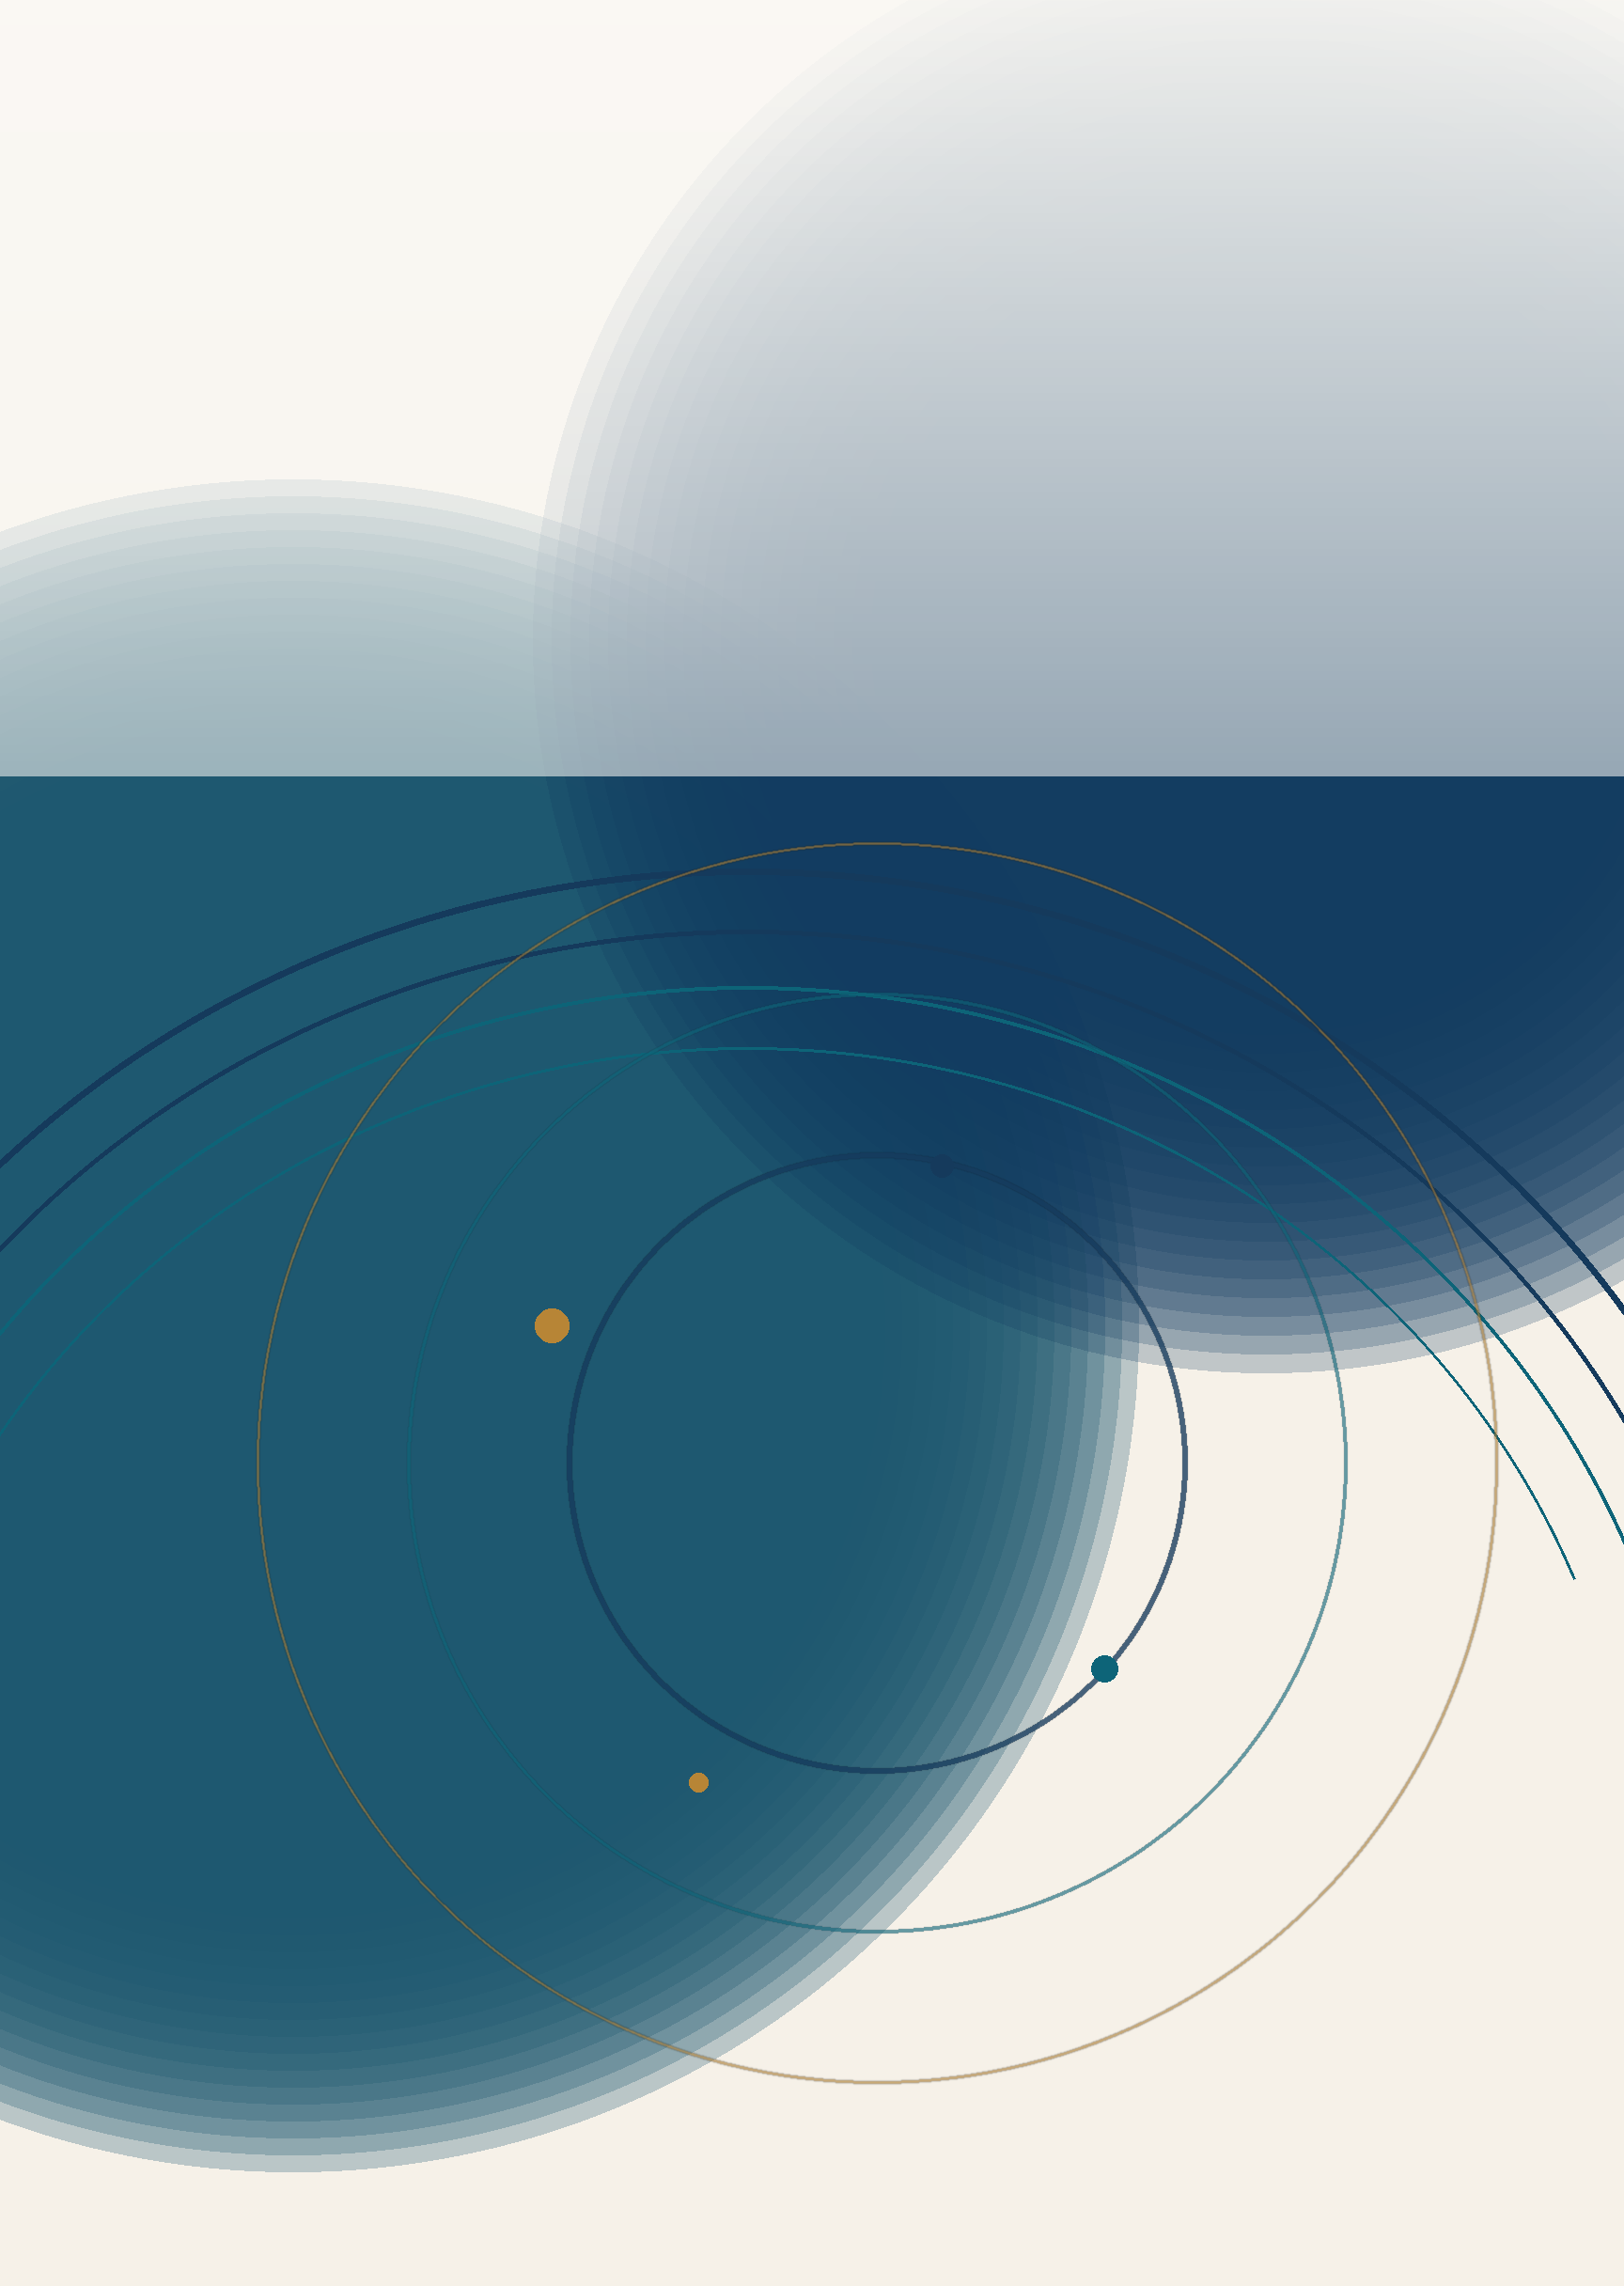
\includegraphics[height=\paperheight,keepaspectratio]{../../../generated_course_notes/core/cosmology/2009_winter_legacy_cosmology/assets/cover-art.png}%
  };
  \node[
    anchor=north west,
    align=left,
    text width=0.78\paperwidth,
    fill=white,
    fill opacity=0.9,
    rounded corners=8pt,
    inner xsep=10pt,
    inner ysep=8pt
  ] at ([xshift=0.08\paperwidth,yshift=-0.06\paperheight]current page.north west) {%
    {\fontsize{30}{33}\selectfont\bfseries\color{black!88} 우주론\\[0.85em]}
    {\large\color{black!72} 한국어판 / 2009년 겨울 · 이전 우주론 강의}
  };
  \node[
    anchor=south west,
    align=left,
    text width=0.68\paperwidth,
    fill=white,
    fill opacity=0.82,
    text opacity=1,
    rounded corners=6pt,
    inner sep=12pt
  ] at ([xshift=0.08\paperwidth,yshift=0.08\paperheight]current page.south west) {%
    {\normalsize\color{black!78} 원 강의: Leonard Susskind\\[0.35em]}
    {\small\color{black!72} 보조 강의 노트: \href{https://lazying.art}{LazyingArt LLC} / \href{https://github.com/lachlanchen/Video2Book}{Video2Book}}
  };
\end{tikzpicture}
\mbox{}
\end{titlepage}
\hypersetup{pageanchor=true}

\clearpage
\chapter{이 노트에 관하여}
이 독립적으로 편집된 동반 강의 노트는 Leonard Susskind의 강의를 따라 구성했다. 기계 생성 녹취록과 자막, 일부 칠판 화면을 바탕으로 복원한 뒤 이용 가능한 원자료와 대조해 확인했다. 이 노트는 Susskind 교수가 직접 쓴 원고가 아니며, 그의 검토나 승인을 받지 않았다.

이 판본은 \href{https://lazying.art}{LazyingArt LLC}가 오픈 소스 \href{https://github.com/lachlanchen/Video2Book}{Video2Book} 워크플로를 사용해 편집했다. 기계 생성 녹취록은 별도로 제공되며 인식 오류가 있을 수 있다. 편집상 보충 설명과 중요한 내용을 재구성한 부분은 각주에 표시했다.
\clearpage
\tableofcontents
\mainmatter
\chapter{팽창하는 우주의 기하학}

여기서 다루는 것은 팽창하는 우주와 그 기하학이다. 팽창을 일으키는 요인을 묻기에 앞서 공간이 팽창한다는 것이 무엇을 뜻하는지 설명하는 것이 목표다. 뉴턴 역학의 \(F=ma\) 우주론은 나중에 다루며, 그 뒤에야 기하학과 동역학을 합쳐 완전한 프리드먼--로버트슨--워커 체계를 구성한다.

\section{팽창하는 직선 위의 공변 좌표}

가능한 한 단순한 예인 시공간이 아닌 1차원 공간에서 시작하자. 은하들이 일정한 간격으로 놓인 무한한 직선을 상상해 보자. 좌표 \(x\)는 아직 물리적 거리를 재지 않는다. 은하에 이름표를 붙일 뿐이다. \(x\)를 은하의 이름이라고 생각해도 좋다. 배열 전체가 늘어나거나 줄어들더라도 그 이름은 은하에 계속 붙어 있다.

\(x=0\)라고 불리는 은하에서 \(x=1\)이라고 불리는 은하까지의 물리적 거리를 \(a\)라고 하자. 그러면 임의의 두 은하 사이의 물리적 거리는
\begin{equation}
d=a\,\Delta x.
\end{equation}
좌표 차이 \(\Delta x\)는 이름표 사이의 차이일 뿐이다. 인자 \(a\)는 그 이름표 차이를 미터자로 잰 실제 거리로 바꿔 준다.

이제 직선이 늘어나는 탄성 실이라고 상상해 보자. 이름표는 은하에 붙어 있지만, 이웃 은하 사이의 거리는 시간에 따라 변한다. 같은 관계식은 다음과 같이 된다.
\begin{equation}
d(t)=a(t)\,\Delta x.
\end{equation}
이 단계에서 균질성이란 공통 간격이 시간에 따라 변할 수는 있어도 이웃 은하들이 어디서나 같은 간격으로 떨어져 있다는 뜻일 뿐이다.

\section{허블 법칙과 중심의 부재}

고정된 두 은하의 상대 속도를 구하려면 두 은하를 고정해 \(\Delta x\)가 시간에 따라 변하지 않게 하자. 미분하면
\begin{align}
\dot d &= \dot a\,\Delta x \\
       &= \frac{\dot a}{a}\,a\,\Delta x \\
       &= \frac{\dot a}{a}\,d.
\end{align}
이제 다음과 같이 정의하면
\begin{equation}
H(t)\equiv \frac{\dot a}{a},
\end{equation}
다음 관계를 얻는다.
\begin{equation}
\dot d = H(t)\,d.
\end{equation}
이것이 허블 법칙이다.

역사적으로 쓰인 ``허블 상수''라는 표현은 오해를 부른다. 이 양은 시간에 대해서가 아니라 공간에 대해 일정하다. 주어진 순간에는 모든 은하에서 같지만, 일반적으로 우주가 진화함에 따라 변한다. 허블 매개변수라고 부르는 편이 더 적절하다.

이 법칙에 따르면 더 멀리 있는 은하일수록 더 빠르게 멀어진다. 하지만 이 법칙은 어떤 중심도 특정하지 않는다. 논의의 어떤 부분도 \(x=0\)나 다른 어느 점도 특별하게 취급하지 않는다. 모든 관측자는 같은 법칙을 본다. 따라서 이 모형의 팽창하는 우주는 특별히 지정된 한 장소에서 일어난 폭발이 아니다.

적색편이는 곧바로 등장한다. 서로 멀어지는 두 은하가 빛 신호를 주고받으면, 수신된 빛은 적색편이를 겪는다. 후퇴 속도가 클수록 적색편이도 크다. 따라서 스펙트럼선은 후퇴 속도에 관한 정보를 알려 준다. 거리를 재기는 더 어렵고, 허블의 초기 추정치는 거칠었다. 그의 첫 그래프는 완벽한 직선이 아니라 불확실성이 큰 점들이 흩어져 있는 그래프였다. 그래도 잡음 속에서 기하학적 원리는 살아남았다. 후퇴 속도는 거리에 비례한다.

\begin{classroomqa}\audiencequestion{은하들이 충분히 멀리 떨어져 있으면 허블 법칙에 따라 광속보다 빠르게 움직이나요?}\lecturetimestamp{00:20:23}\lecturerresponse{네, 이 후퇴의 의미에서는 그렇습니다. 하신 말씀은 맞습니다. 이 문제는 꼭 다시 다루겠습니다. 가장 중요한 내용 가운데 하나입니다.}\end{classroomqa}

\section{고차원, 등방성, 그리고 \(a(t)\)의 시간 의존성}

공간 차원을 더해도 본질적으로 달라지는 것은 없다. 2차원에서는 \((x,y)\)로 표시한 은하들의 정사각 격자를, 3차원에서는 \((x,y,z)\)로 표시한 격자를 상상해 보자. 여기서도 좌표는 동행하는 이름표다. 좌표는 물리적 거리를 직접 재는 대신 은하와 함께 움직인다.

\(x\) 방향의 간격과 \(y\) 방향의 간격이 같아야 하는 이유는 무엇일까? 답은 관측에 있다. 은하들이 한 방향에서 체계적으로 더 빽빽하다면 하늘은 방향에 따라 다르게 보일 것이다. 충분히 큰 규모에서는 그렇지 않다. 이처럼 방향에 따라 달라지지 않는 성질이 등방성이다.

2차원에서 두 은하 사이의 거리는
\begin{equation}
d=a\sqrt{(\Delta x)^2+(\Delta y)^2},
\end{equation}
3차원에서는
\begin{equation}
d=a\sqrt{(\Delta x)^2+(\Delta y)^2+(\Delta z)^2}.
\end{equation}
고정된 은하 쌍에서는 좌표 차이가 일정하므로, 다시 미분하면
\begin{equation}
\dot d=\frac{\dot a}{a}\,d.
\end{equation}
허블 법칙은 그대로다.

균질성은 장소에 따른 동일성을 뜻한다. 등방성은 방향에 따른 동일성을 뜻한다. 어느 쪽도 작은 규모에서 정확히 성립하지는 않는다. 은하수를 바라보는 것과 그 원반 바깥을 바라보는 것은 다르고, 개별 은하들도 짧은 거리 규모에서는 균일하게 퍼져 있지 않다. 그러나 많은 은하에 대해 평균을 내면 큰 규모의 우주는 대략 어디서나, 어느 방향으로나 비슷해 보인다.

\begin{classroomqa}\audiencequestion{속도가 거리에 비례하고 거리가 늘어나고 있다면, 고정된 한 쌍의 은하들은 서로 가속하며 멀어지는 건가요?}\lecturetimestamp{00:40:22}\lecturerresponse{아닙니다. 허블 법칙은 주어진 순간의 후퇴 속도가 거리에 비례한다고 말합니다. 고정된 한 쌍의 은하 사이 속도가 시간에 따라 증가하는지 감소하는지는 그 자체로 말해 주지 않습니다. 그것은 \(a(t)\)의 구체적인 시간 의존성에 달려 있습니다. \(a(t)\propto t\)이면 이웃 은하들은 일정한 속도로 멀어집니다. \(a(t)\propto t^2\)이면 고정된 은하 쌍의 후퇴 속도는 시간에 따라 증가합니다. \(a(t)\propto \log t\)이면 후퇴 속도는 시간에 따라 감소합니다. 거리의 함수로서 법칙 \(\dot d=(\dot a/a)d\)은 언제나 성립하지만, 가속과 감속은 별개의 문제입니다.}\end{classroomqa}

오랫동안 우주론자들은 우주가 감속하고 있으리라 예상했다. 중력이 위로 던진 물체의 속도를 늦추듯, 초기 팽창도 늦출 것이라고 보았기 때문이다. 여기서 짚을 점은 허블 법칙만으로는 \(\dot a\) 또는 \(\ddot a\)의 거동을 결정할 수 없다는 것뿐이다.

\begin{classroomqa}\audiencequestion{척도인자 \(a\)의 초기값은 어떻게 정하나요?}\lecturetimestamp{00:46:18}\lecturerresponse{전체적인 정규화는 임의적입니다. 물리적으로 중요한 것은 \(a\) 자체의 수치적 크기가 아니라 그것이 어떻게 변하는가입니다. 다른 척도인자 \(b=3a\)를 정의하면 \(\dot b/b=\dot a/a\)입니다. \(a\)에 상수를 곱해 재척도화해도 관례나 단위만 바뀔 뿐 허블 매개변수는 바뀌지 않습니다.}\end{classroomqa}

\section{공간 계량에서 시공간 계량으로}

이제 \(\Delta x\)를 \(dx\)로 바꾸자. 이웃한 점들 사이의 물리적 거리는
\begin{equation}
ds=a\,dx,
\end{equation}
따라서
\begin{equation}
ds^2=a^2\,dx^2.
\end{equation}
이것이 1차원 공간의 계량이다. \(dx^2\)의 계수는
\begin{equation}
g_{xx}=a^2.
\end{equation}
그러므로 팽창하는 우주는 계량의 공간 부분이 시간에 의존한다고 표현할 수 있다.

공간에서 시공간으로 넘어가려면 상대론적 간격을 쓰자. 1차원 공간에서는
\begin{equation}
d\tau^2=dt^2-a^2(t)\,dx^2.
\end{equation}
동행 관측자에게는 \(dx=0\)이므로 \(d\tau=dt\)이다. 보통의 우주 시간은 은하와 함께 움직이는 시계가 측정하는 고유 시간이다.

이 시점의 칠판 그림은 동행 세계선과 선요소, 계량 표기를 한데 보여 주므로 유용하다.
\begin{figure}[H]\centering
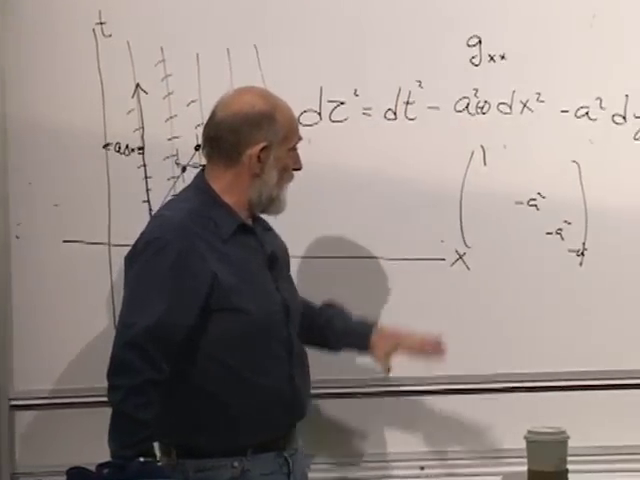
\includegraphics[width=0.82\textwidth]{lecture_01_figure_02.png}\caption{팽창하는 1차원 우주의 동행 세계선과 이에 대응하는 시공간 간격.}\end{figure}

세 공간 차원에서는 같은 양상을 바탕으로 신중하게 다음과 같이 확장할 수 있다.\footnote{판서의 일부는 00:56:38--00:58:51 무렵 가려져 있다. 이 세 차원 형태는 한 공간 차원에서 세 공간 차원으로 확장한다는 설명과 판서에 보이는 대각선 패턴을 함께 따른다.}
\begin{equation}
d\tau^2=dt^2-a^2(t)\bigl(dx^2+dy^2+dz^2\bigr),
\end{equation}
대각 계량은 다음과 같이 주어진다.
\begin{equation}
g_{\mu\nu}=\mathrm{diag}\bigl(1,-a^2,-a^2,-a^2\bigr).
\end{equation}
비대각 성분은 사라진다.
\begin{equation}
g_{tx}=g_{ty}=g_{tz}=0.
\end{equation}

균질성이란 계량 계수들이 시간에는 의존할 수 있지만 공간상의 위치에는 의존하지 않는다는 뜻이다. 등방성이란 세 공간 방향이 같은 방식으로 들어간다는 뜻이다.

\begin{classroomqa}\audiencequestion{\(dx\)를 거리라고 생각해야 하는 것 아닌가요?}\lecturetimestamp{01:01:18}\lecturerresponse{아닙니다. \(dx\)는 거리가 아닙니다. \(a\,dx\)가 거리입니다. \(dx\)는 단지 좌표 간격입니다. 이를 이해하는 한 가지 좋은 방법은 누군가 어느 순간 은하들 사이에 좌표 격자를 그린 다음 그 격자가 은하들을 따라가도록 정했다고 상상하는 것입니다. 그렇게 정했으므로 좌표 간격은 고정되어 있지만 물리적 거리는 변합니다. 거리 단위를 \(x\) 대신 \(a\)에 넣어도 됩니다. 이는 관례의 문제입니다. 중요한 것은 곱 \(a\,dx\)입니다.}\end{classroomqa}

\begin{classroomqa}\audiencequestion{\(dt^2\)의 계량 계수가 \(1\)과 같습니다. 이것도 단지 관례인가요?}\lecturetimestamp{01:03:24}\lecturerresponse{네. 그 자체로는 물리적인 의미가 없습니다. 계수가 시간에만 의존한다면 시간 변수를 바꾸어 그 계수를 단순히 \(dt^2\)로 만들 수 있습니다. 마찬가지로 \(c=1\)인 단위를 택할 수도 있습니다. 여기서 관례가 아닌 것은 계수가 위치에는 의존하지 않는다는 점입니다. 다만 시간에는 의존할 수 있습니다.}\end{classroomqa}

\begin{classroomqa}\audiencequestion{이것을 아인슈타인 장방정식에 넣으면 에너지-운동량 텐서는 어떻게 되나요?}\lecturetimestamp{01:05:59}\lecturerresponse{그것은 다음 종류의 질문이지만, 지금 논의하는 내용이 아니라 동역학에 속합니다. 이 계량을 아인슈타인 방정식에 넣고 어떤 에너지-운동량 분포가 해를 만들지 물을 수 있습니다. 아주 중요한 문제지만, 지금 다루는 주제는 동역학이 아니라 기하학입니다.}\end{classroomqa}

\section{지평선이 가리는 것}

큰 규모의 우주가 균질하고 등방적이라는 가정은 근사적으로만 다룬다. 별이나 행성, 심지어 개별 은하의 규모에서 우주는 분명 균질하지 않다. 국소적인 관측에서도 정확히 등방적이지는 않다.

농부의 밭을 생각하면 규모에 따른 차이를 이해할 수 있다. 한 규모에서는 규칙적으로 보이지만, 훨씬 작은 규모에서는 분명 그렇지 않다. 밭 전체보다 더 큰 규모에서는 다시 균질해 보이지 않는다. 우주론도 마찬가지다. 많은 은하에 대해 평균을 내면 큰 규모의 분포는 대략 균일해 보인다. 충분히 작은 규모에서는 그렇지 않다.

우주는 우리가 볼 수 있는 영역보다 크고, 우리가 앞으로도 볼 수 있는 영역보다 크다. 실제로 탐사할 수 있는 규모에서 우주는 국소적인 변화를 제외하면 등방적이고 균질하다. 그 바깥에 대해서는 직접 관측으로 보장되는 것이 없다.

\begin{classroomqa}\audiencequestion{우리가 정말 직접 알아낼 수는 없다고 하셨는데요. 그렇다면 간접적으로 알아낼 방법은 있을 수도 있나요?}\lecturetimestamp{01:10:34}\lecturerresponse{그럴 수도 있습니다. 요즘에는 충분히 큰 규모에서 우주가 균질하지 않다고 보는 견해가 대부분이며, 저도 그렇게 생각합니다. 하지만 제가 이 내기를 이기지도 지지도 않을 거라고 봅니다. 근본적이고 기본적인 이유 때문에 지금 볼 수 있는 곳보다 훨씬 더 멀리 볼 수는 없기 때문입니다. 지평선이 존재한다는 것이 바로 그 이유입니다.}\end{classroomqa}

\begin{classroomqa}\audiencequestion{중력을 이용하면 보이지 않는 곳 너머의 질량을 찾아낼 수 있지 않나요?}\lecturetimestamp{01:11:53}\lecturerresponse{아닙니다. 멀리 있는 질량은 우리를 단지 자유낙하 상태로 만들 수도 있습니다. 창문 없는 방에 앉아 있는 우리는 태양의 중력장 안에서 태양 주위를 공전하지만, 밖을 보지 못한다면 태양이 있다는 사실을 알아내기 어렵습니다. 조석력만이 태양의 존재를 드러내며, 원천이 충분히 멀리 있으면 그 조석 효과는 너무 작아 감지할 수 없을 수도 있습니다.}\end{classroomqa}

따라서 지평선은 직접 지식에 대한 궁극적인 장벽이다. 그는 우주의 부피가 우리가 앞으로도 볼 수 있는 영역의 부피보다 적어도 천 배는 크다고 사실상 확신하면서 말하고, 그 주장의 이유는 나중으로 미룬다.

\section{경계 없이 유계인 공간}

이제 닫힌 기하학을 살펴보자. 무한 직선은 열려 있고 비유계다. 선분은 범위가 유한하다는 의미에서 유계다. 유계라는 말은 경계가 있다는 뜻이 아니라 범위가 유한하다는 뜻이다.

벽이 있는 정육면체는 적절한 예가 아니다. 벽 가까이에 있는 사람과 벽에서 먼 사람은 동등하지 않으므로 균질성을 위배한다. 중심에 있는 사람조차 방향에 따라 다른 것을 보므로 등방성도 위배한다.

원이나 공의 내부도 적절하지 않다. 중심에 있는 사람은 모든 방향에서 같은 것을 보지만, 그런 대칭성을 지닌 곳은 특별한 한 점뿐이다. 중심에서 벗어나면 한 방향으로는 벽이 가깝고 다른 방향으로는 멀다. 따라서 일반적인 관측자에게 공간은 균질하지도 등방적이지도 않다.

아주 큰 규모에서는 우주가 균질하고 등방적이라는 가정을 기본으로 삼는다. 이것이 우주론적 원리다. 유용한 가정이지만 수정될 가능성에서 자유롭지는 않다.

\begin{classroomqa}\audiencequestion{모든 곳에서 등방적이면 균질하다는 뜻인가요?}\lecturetimestamp{01:18:57}\lecturerresponse{네. 모든 관측자가 모든 방향에서 같은 것을 본다면 균질성도 따른다는 뜻입니다. 그러나 그 역은 성립하지 않습니다. 균질하다고 해서 등방적인 것은 아닙니다. 예를 들어 우주 전체에 화살표가 모두 같은 방향을 가리키며 차 있다고 하면, 우주는 균질하면서도 선호되는 방향을 가질 수 있습니다.}\end{classroomqa}

적절한 유계 모형은 아무 특징도 없는 구의 표면이다. 그 표면에 갇혀 사는 2차원 생명체에게는 세계가 유한한데도 모든 장소가 국소적으로 서로 같고 모든 방향도 서로 같다. 이것이 경계 없이 유한한 공간이다.

\section{원 위의 닫힌 1차원 우주}

대수를 단순하게 하려고 구의 예를 한 공간 차원으로 줄여 원 위에서 살아가는 경우를 생각하자. 1차원에서 등방성은 왼쪽과 오른쪽이 동등하다는 뜻이다. 원은 정확히 그런 성질을 지닌다. 한 점을 택해 \(\theta=0\)라고 하자. 나머지 모든 점은 라디안으로 측정한 각좌표 \(\theta\)로 표시한다. 원점 바로 한쪽에 있는 점은 작은 음의 각도로도, \(2\pi\)에 조금 못 미치는 각도로도 나타낼 수 있다. 이러한 주기성은 기하학의 일부다.

원 위의 거주자들이 다룰 수 있는 것은 원주뿐이며, 바깥쪽의 반지름이나 중심은 대상이 아니다. 원을 따라 걸어 처음 출발한 점으로 돌아올 때까지 이동하면 전체 길이를 잴 수 있다. 원을 주변의 평면에 그리면 반지름과 비슷한 양을 도입할 수도 있지만, 그것은 매장 그림에 속하며 그들이 재는 내재적 기하학에는 속하지 않는다.

여기서 칠판 그림은 각도 좌표와 전체 원주를 한 그림에 보여 주므로 유용하다.
\begin{figure}[H]\centering
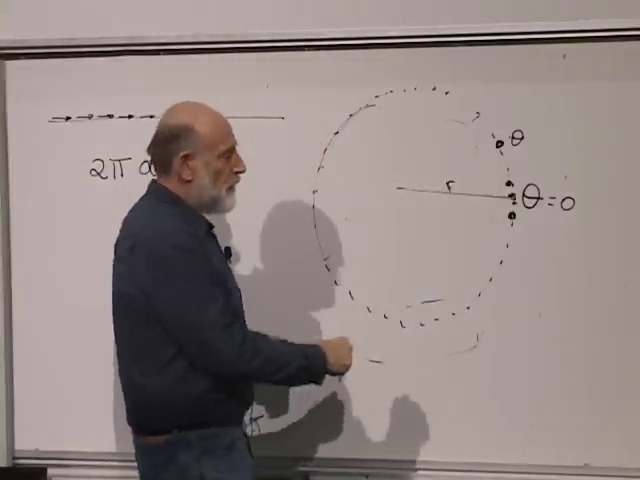
\includegraphics[width=0.82\textwidth]{lecture_01_figure_03.png}\caption{전체 원주가 \(2\pi a\)인 닫힌 1차원 우주의 각도 표현.}\end{figure}

편리한 관례는 다음과 같다.\footnote{01:26:40--01:29:20 주변에서는 전체 원주 자체를 척도인자로 놓는 경우와 이를 \(2\pi a\)로 쓰는 경우가 잠시 혼용된다. 뒤의 관례가 호 길이 공식으로 이어지는 표기이므로 여기서는 이를 사용한다.}\begin{equation}
L=2\pi a,
\end{equation}여기서 \(L\)는 전체 원주다.

작은 각도 간격 \(\Delta\theta\)에 대해 물리적 거리는
\begin{equation}
d=a\,\Delta\theta.
\end{equation}
무한소로 가면
\begin{equation}
ds=a\,d\theta,
\end{equation}
따라서
\begin{equation}
ds^2=a^2\,d\theta^2.
\end{equation}
이것이 원 위의 국소 계량이다.

\(a\)가 시간에 따라 변하면 닫힌 1차원 우주는 팽창하거나 수축한다. 고정된 은하 쌍에 대해
\begin{equation}
d(t)=a(t)\,\Delta\theta,
\end{equation}
따라서
\begin{equation}
\dot d=\dot a\,\Delta\theta
      =\frac{\dot a}{a}\,d.
\end{equation}
여기에서도 허블 법칙은 성립한다. 다만 원의 반대쪽으로 가는 경로가 모호해질 정도로 멀리 떨어지지 않은 은하 쌍에 한해서다.

시공간 계량은 다음과 같다.
\begin{equation}
d\tau^2=dt^2-a^2(t)\,d\theta^2.
\end{equation}
\(a\)가 일정하면 시공간 그림은 원기둥이다. \(a\propto t\)이면 원뿔이다. \(a(t)\)가 더 불규칙하게 변하면 그림은 꽃병 모양이 된다.

그림을 거꾸로 따라가면 은하들이 점점 더 가까워진다. 원주를 따라 \(360\)개의 은하가 있다고 하면, 나중에는 서로 널찍이 퍼져 있고 더 이른 때에는 아주 가까워지며, 그보다 더 이른 때에는 더욱 가까워진다. 결국 은하들은 더 이상 서로 분리된 은하가 아니게 되고, 그보다 더 이른 때에는 서로 분리된 원자조차 아니게 된다. 그래도 공간의 특별한 점은 없다.

이 모형에서 빅뱅이 어디에서 일어났는가라는 질문에 가장 명확히 답하면 이렇다. \(a(t)\to 0\)일 때 모든 두 점 사이의 거리 \(a(t)\,\Delta\theta\)는 0으로 간다. 우주 전체가 모든 곳에서 동시에 작아진다. 은하들은 외부 공간의 특권적인 한 장소에서 날아가고 있는 것이 아니다. 기하학 자체의 척도가 변하고 있다. 그런 의미에서 답은 어디에서나이다.

\begin{classroomqa}\audiencequestion{시공간이 휘어 있다고 하셨는데, 원기둥이라면 휘어 있나요?}\lecturetimestamp{01:38:04}\lecturerresponse{아닙니다. 원기둥이라면 휘어 있지 않습니다. 이 경우에는 \(a\)가 시간에 따라 일정합니다. 더 높은 차원의 공간에 그려져 있어서 휘어 보일 뿐입니다. 원기둥을 잘라 펼치면 늘이지 않고도 평평하게 놓을 수 있습니다.}\end{classroomqa}

이어서 원뿔을 살펴보자. \(a\propto t\)이면 시공간 그림은 원뿔이다. 원뿔의 꼭짓점에서 떨어진 부분도 같은 내재적 의미에서 평평하다. 펼쳐서 평면으로 만들 수 있다. 꼭짓점은 다르다. 그곳은 원뿔 특이점이다.

다음 단계에서는 구형 우주의 기하학을 살펴본 뒤, \(a(t)\)가 어떻게 커지거나 작아지는지 결정하는 동역학을 다룬다.
\chapter{뉴턴 우주론과 프리드만 방정식}

지난 시간에는 공간의 계량에 관해 이야기했습니다. 다음 질문은 동역학입니다. 스케일 인자는 시간에 따라 어떻게 변할까요? 먼저 간단한 기하학을 살펴본 뒤 뉴턴 우주론으로 넘어가겠습니다. 여기서는 일반 상대성 이론으로부터 프리드만 방정식을 유도하지 않습니다. 뉴턴 방정식으로 유도하겠습니다.

\section{균질성, 등방성과 시간에 따라 변하는 계량}

균질성과 등방성을 기본 가정으로 둡니다. 우주가 균질하고 등방적이며 시간에 따라 변한다면 허블 법칙은 언제나 성립합니다. 어느 한 시각을 고정하면 후퇴 속도는 거리에 비례합니다.
\begin{equation}
v = H(t)\,d.
\end{equation}
비례 관계는 선형입니다. 일정한 것은 시간이 아니라 공간입니다. 주어진 순간에는 어디에서나 같은 비례 상수가 적용됩니다.

\begin{classroomqa}
\audiencequestion{선형 비례한다는 뜻인가요?}\lecturetimestamp{00:02:06}
\lecturerresponse{그렇습니다. 시각을 고정하면 후퇴 속도는 거리에 선형 비례합니다. 비례 상수가 허블 상수입니다. 일반적으로 이 값은 시간에 따라 달라지지만 공간상의 위치에 따라 달라지지는 않습니다.}
\end{classroomqa}

그래서 ``허블 상수''라는 표현은 주의해서 써야 합니다. 공간상의 위치에 대해서는 상수입니다. 시간에 대해서는 상수가 아닙니다.

자연스럽게 이런 질문이 나옵니다. 공간이 팽창한다면 왜 미터 자도 함께 늘어나지 않을까요? 원자 규모에서 미터 자를 결속하는 힘은 우주 팽창과 관련된 어떤 효과보다도 압도적으로 강하기 때문입니다. 결합된 물체는 결합된 상태를 유지합니다. 팽창하는 것은 충분히 떨어져 있어 서로 강하게 붙잡고 있지 않은 은하들 사이의 거리입니다.

\begin{classroomqa}
\audiencequestion{측정용 자도 함께 팽창한다는 사실은 문제가 되지 않나요?}\lecturetimestamp{00:04:00}
\lecturerresponse{아닙니다. 측정용 자는 팽창하지 않습니다. 팽창하는 것은 좌표입니다. 미터 자를 결속하는 힘은 팽창에 따른 효과보다 훨씬 강하므로, 보통의 결합된 물체는 배경과 함께 팽창하지 않습니다. 충분히 멀리 떨어진 은하들은 서로 멀어지지만 미터 자는 그렇지 않습니다.}
\end{classroomqa}

원자 사이에 아주 작은 추가적인 척력 효과가 있다고 상상해 볼 수도 있습니다. 그래도 막대를 잡아당겨 부러뜨리지는 못합니다. 단지 평형 간격을 조금 바꿀 뿐입니다. 작은 추가 힘이 단단한 용수철의 평형 위치를 약간 바꾸는 것과 같습니다.

\begin{classroomqa}
\audiencequestion{그렇지만 점들 사이의 힘으로 모델링할 수는 없는 거죠? 그렇지 않으면 가속도가 생길 테니까요.}\lecturetimestamp{00:05:29}
\lecturerresponse{원자 사이에 작은 추가 힘이 있다고 상상할 수는 있습니다. 다만 그 힘이 결합력에 비해 아주 작다면 평형 위치만 조금 바뀝니다. 팽창 자체가 보통의 힘 법칙을 만들어 내지는 않습니다. 일부 팽창은 힘으로 모델링할 수 있는데, 가속 팽창이 그 예입니다. 하지만 그것은 나중에 다룰 문제입니다.}
\end{classroomqa}

따라서 유용한 좌표는 팽창하는 물질 분포에 붙어 있는 좌표입니다. 별도의 특이 속도가 없는 은하들은 같은 좌표값을 유지합니다. 시간에 따라 변하는 것은 좌표 간격과 미터 단위로 측정한 물리적 거리 사이의 관계입니다. 이 관계를 스케일 인자 \(a(t)\)로 나타냅니다.

평탄한 공간에서는 공간 계량을 다음과 같이 쓸 수 있습니다.
\begin{equation}
ds^2 = a(t)^2\left(dx^2+dy^2+dz^2\right).
\end{equation}
여기서 \(a\)는 좌표 거리 한 단위만큼 떨어진 이웃한 점들 사이의 실제 거리이며, 미터 단위로 측정합니다. 우주가 팽창하면 \(a\)는 시간에 따라 변합니다.

시공간으로 확장하려면 특수 상대론의 형태
\begin{equation}
d\tau^2 = dt^2 - ds^2,
\end{equation}
에서 출발해 공간 계량을 대입합니다. 그러면 다음을 얻습니다.
\begin{equation}
d\tau^2 = dt^2 - a(t)^2\left(dx^2+dy^2+dz^2\right).
\end{equation}
계수는 공간상의 위치에 의존하지 않고 시간에만 의존합니다. 이것이 계량의 언어로 표현한 균질성입니다. 대각 계량은 다음과 같은 형태입니다.
\begin{equation}
g_{\mu\nu}=\mathrm{diag}\!\left(1,-a(t)^2,-a(t)^2,-a(t)^2\right).
\end{equation}
\editorialnote{여기에 적힌 전체 대각 행렬은 00:14:33 전후의 강의에서 설명한 계량 텐서의 형태를 나타냅니다. 칠판 화면에는 선요소가 선명하게 보이지만, 행렬 전체를 판독할 수 있을 만큼 선명하지는 않습니다.}

비대각 항은 없습니다. \(dx\,dy\)도, \(dx\,dt\)도, 다른 혼합 항도 없습니다. 계량은 평탄한 시공간의 계량만큼이나 단순합니다. 특이한 점은 공간 측도와 시간 사이의 관계 자체가 시간에 따라 변한다는 것입니다.

\begin{figure}
\centering
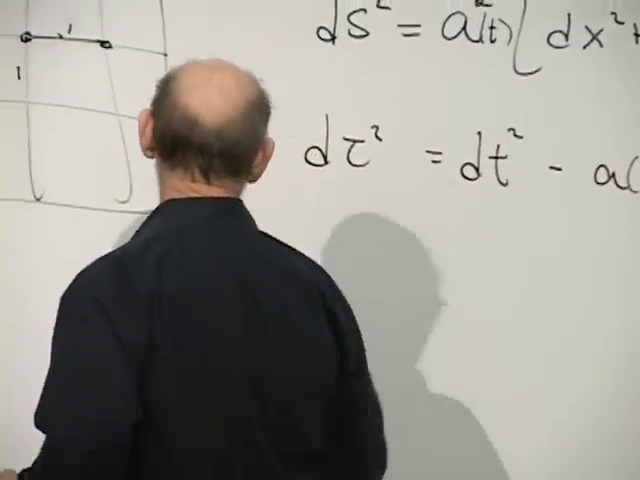
\includegraphics[width=0.62\textwidth]{lecture_02_figure_02.png}
\caption{동행 좌표 격자 스케치와 시간에 따라 변하는 스케일 인자를 포함한 시공간 간격.}
\end{figure}

그림이 요점을 잘 보여 줍니다. 앨리스와 밥은 동행 좌표계에서 계속 한 단위만큼 떨어져 있지만, 그 좌표 한 단위가 나타내는 미터 거리는 시간이 흐를수록 커집니다. 과거 어느 시점에 \(a(t)\)가 0이었다면 모든 물리적 거리가 0이었을 것입니다. 모든 것이 서로 위에 눌려 포개져 있었을 것입니다. 그래서 \(a\to 0\)는 무한 밀도에 해당합니다. \(a\)가 커질수록 우주는 점점 더 희박해집니다.

이 계량 형태가 모든 좌표계에서 성립하는 것은 아닙니다. 은하들과 함께 움직이는 좌표계에서 성립하는 형태입니다.

\begin{classroomqa}
\audiencequestion{그 방정식의 작은 \(t\), \(a(t)\)에서 \(t\)는 누구의 시간인가요?}\lecturetimestamp{00:19:19}
\lecturerresponse{은하들과 함께 움직이는 시계가 측정하는 시간입니다. 같은 우주 시계 공장에서 만든 똑같은 시계를 은하에 실어 보낸다고 상상해 보세요. 이 좌표계에서 시간 변수는 그 시계들이 측정하는 바로 그 시간입니다. 은하의 세계선에서는 고유 시간이 이 좌표 시간과 같습니다.}
\end{classroomqa}

실제로 동행하는 은하의 세계선을 따라가면,
\begin{equation}
dx=dy=dz=0,
\end{equation}
따라서
\begin{equation}
d\tau^2 = dt^2,
\end{equation}
이고, 그러므로
\begin{equation}
dt=d\tau.
\end{equation}

\begin{classroomqa}
\audiencequestion{이 계량 형태를 불변으로 유지하는 변환이 있나요?}\lecturetimestamp{00:23:08}
\lecturerresponse{회전은 그렇습니다. \(dx^2+dy^2+dz^2\)가 회전에 대해 불변이기 때문입니다. 하지만 로런츠 부스트는 이 형태를 보존하지 않습니다. 물질 자체가 은하들과 함께 움직이는 좌표계를 정하며, 다른 좌표계에서는 우주가 등방적으로 보이지 않을 것입니다.}
\end{classroomqa}

\section{중력장 속 발사체}

뉴턴 역학을 우주 전체에 적용하기 전에 한 걸음 물러나 더 간단한 문제부터 살펴보면 좋습니다. 큰 질량 \(M\), 그보다 훨씬 작은 질량 \(m\), 그리고 처음에 바깥쪽으로 주는 충격량이 있습니다. 충격량을 받은 뒤 작은 질량은 중력장 속에서 움직이며 뉴턴 역학이 예측하는 대로 운동합니다.

우주론 논의에서 중요한 것은 전체 궤도 문제가 아닙니다. 중요한 것은 에너지 보존입니다. 운동 에너지는
\begin{equation}
\frac{1}{2}mv^2.
\end{equation}

\begin{figure}
\centering
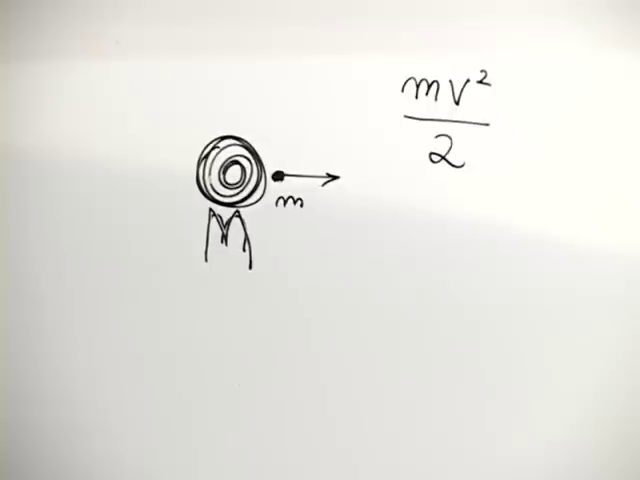
\includegraphics[width=0.42\textwidth]{lecture_02_figure_03.png}
\caption{바깥쪽으로 움직이는 시험 질량과 운동 에너지 항 \(\frac{1}{2}mv^2\).}
\end{figure}

중력 퍼텐셜 에너지에는 두 질량의 곱과 뉴턴 상수가 들어가며, 분모에는 거리의 1승이 들어갑니다. 칠판에 쓴 식에서는 인자들이 \(mMG/D\)의 순서로 나옵니다. 그러므로 여기서도 그 순서를 유지하는 편이 좋습니다.
\begin{equation}
-\frac{mMG}{D}.
\end{equation}
따라서 전체 에너지는
\begin{equation}
\frac{1}{2}mv^2-\frac{mMG}{D}.
\end{equation}
에너지 보존 법칙은 논의 중인 특정 입자에 대해 이 양이 시간에 따라 변하지 않는다는 것만 말해 줍니다. 입자마다 에너지는 다를 수 있습니다.

\begin{figure}
\centering
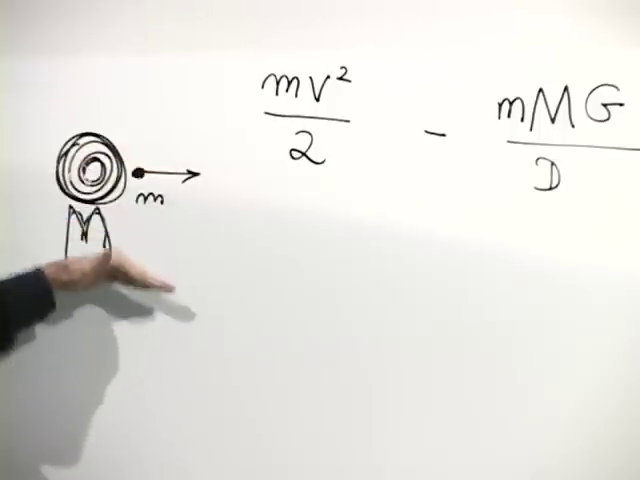
\includegraphics[width=0.62\textwidth]{lecture_02_figure_04.png}
\caption{반지름 방향으로 움직이는 시험 질량의 전체 뉴턴 에너지: 운동 에너지 항에서 중력 퍼텐셜을 뺀 값.}
\end{figure}

음의 부호가 중요합니다. 중력은 인력이므로 중력 퍼텐셜 에너지는 음수입니다. 입자를 더 가까이 가져오면 음의 퍼텐셜 에너지의 크기가 커집니다. 입자를 더 멀리 옮기면 퍼텐셜 에너지는 덜 음수가 됩니다.

\begin{classroomqa}
\audiencequestion{거리에 따라 퍼텐셜 에너지가 감소하는 게 아니라 증가하나요?}\lecturetimestamp{00:34:13}
\lecturerresponse{그렇습니다. 상수는 잠시 잊고 \(1/D\)와 \(-1/D\)의 그래프를 보세요. 힘은 퍼텐셜 에너지가 감소하는 쪽으로 작용합니다. 그러므로 인력은 위아래가 뒤집힌 곡선 \(-1/D\)에 해당합니다. 따라서 입자가 안쪽으로 움직일수록 퍼텐셜 에너지는 거리에 따라 증가하고 더 음수가 됩니다.}
\end{classroomqa}

\begin{figure}
\centering
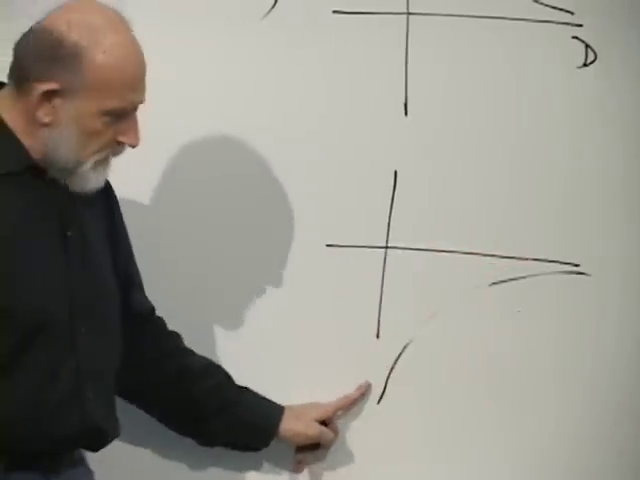
\includegraphics[width=0.46\textwidth]{lecture_02_figure_05.png}
\caption{중력 퍼텐셜 에너지의 부호를 설명하는 \(1/D\)와 \(-1/D\)의 정성적 비교.}
\end{figure}

\section{탈출 속도}

이제 가능한 경우를 분류해 봅시다. 에너지는 양수, 음수 또는 0일 수 있습니다. 경우는 이 세 가지뿐입니다.

\begin{itemize}
\item 에너지가 음수이면 입자는 속박되어 있다. 입자를 위로 던졌을 때 속도가 너무 작으면 입자는 올라가다가 느려지고, 방향을 바꾸어 다시 떨어진다.
\item 에너지가 양수이면 입자는 탈출한다. 중력은 처음에는 입자의 속도를 줄이지만 멈추게 할 정도는 아니며, 결국 입자는 영이 아닌 점근적 바깥쪽 속도로 멀어진다.
\item 에너지가 정확히 영이면 입자는 탈출 속도로 움직인다. 이는 탈출하는 경우와 탈출하지 못하는 경우 사이의 경계 사례다.
\end{itemize}

초기 속도가 충분히 작으면 처음부터 퍼텐셜 항이 우세하여 에너지가 음수입니다.

\begin{figure}
\centering
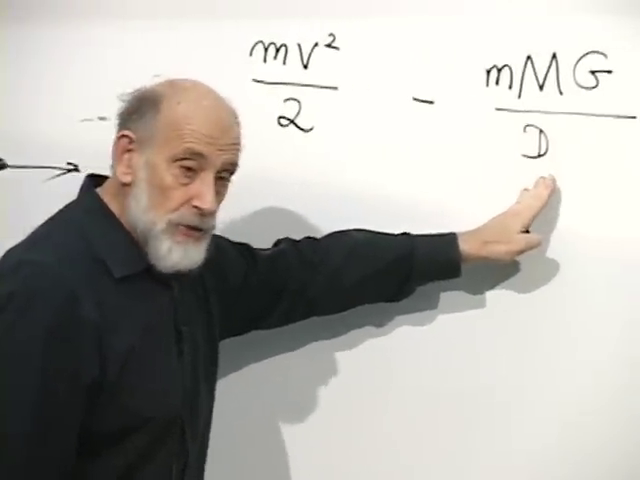
\includegraphics[width=0.62\textwidth]{lecture_02_figure_06.png}
\caption{작은 바깥쪽 속도에서는 음의 퍼텐셜 항이 전체 에너지를 좌우한다.}
\end{figure}

에너지가 0인 경우 거리는 계속 커지지만 속도는 계속 줄어듭니다. 입자는 유한한 시간 안에 정지할 수 없습니다. 만약 정지한다면 다시 안쪽으로 떨어질 것입니다. 따라서 거리는 상한 없이 커지는 반면 속도는 0에 가까워집니다.

우주론에서 중요한 직접적인 비유가 바로 이것입니다. 우주도 같은 방식으로 거동할 수 있습니다. 초기의 바깥쪽 허블 흐름이 충분히 크면 모든 것이 서로를 벗어나 멀어집니다. 너무 작으면 중력이 이겨 우주는 거대한 수축에 이릅니다. 탈출 속도와 정확히 유사한 경계 사례도 있습니다.

\section{뉴턴 정리}

우주론 문제를 단순화할 수 있는 것은 역제곱 법칙에 관한 뉴턴 정리 덕분입니다.

물질이 어떤 중심을 기준으로 구대칭 분포를 이룬다면, 분포 바깥에 있는 입자가 받는 중력은 모든 질량이 중심에 모여 있는 경우와 정확히 같습니다. 하지만 정리는 그보다 더 강한 내용을 담고 있습니다. 입자가 분포 안에 있으면 더 작은 반지름 안쪽의 질량만 기여합니다. 더 큰 반지름에 있는 질량은 알짜 힘을 만들지 않습니다.

정리를 가장 깔끔하게 보여 주는 경우는 얇은 구각입니다. 완전한 구형 껍질은 중심에서 벗어난 곳을 포함해 그 내부 어디에 있는 입자에도 중력을 전혀 가하지 않습니다. 처음에는 놀라운 결과처럼 보이지만 \(1/r^2\) 법칙에서는 사실입니다.

\begin{classroomqa}
\audiencequestion{방금 든 예에서 입자가 경계를 가로지를 때 힘이 불연속적으로 변하는 것처럼 보이는데, 이를 조금 의아하게 여겨야 하지 않을까요?}\lecturetimestamp{00:48:19}
\lecturerresponse{그렇습니다.
이상적인 무한히 얇은 껍질이라면 놀라운 일이며, \(1/r^2\) 힘 법칙에서만 나타나는 특성입니다.
실제 껍질에는 두께가 있으므로 변화가 매끄럽게 이어지지만, 이상적인 껍질에 관한 이 명확한 진술이 바로 뉴턴 정리의 놀라운 성질입니다.}
\end{classroomqa}

그림을 보면 이 정리가 그럴듯하게 느껴집니다. 점질량을 물의 점원으로 바꾸어 생각해 봅시다. 3차원에서는 바깥쪽 흐름이 \(1/r^2\)처럼 감소합니다. 이런 점원들을 구형 껍질을 따라 연속적으로 배치해 보세요. 껍질 바깥에서는 모든 물이 중심에 모여 있는 것과 흐름이 정확히 같습니다. 껍질 안에는 중심에 원천이 없으므로 알짜 흐름이 있을 수 없습니다. 중력 정리의 바탕에도 같은 구조가 있습니다.

여기서 요점은 정리를 다시 유도하는 것이 아니라 활용하는 것입니다.

\section{균질한 우주를 하나의 물체 문제로 보기}

이제 우주론으로 돌아갑시다. 은하가 균일한 기체처럼 채워진 작은 우주 영역을 생각해 봅시다. 원한다면 그 중심에 자신을 둘 수 있습니다. 이는 편의를 위한 선택일 뿐입니다. 누구나 자신을 중심에 있다고 정할 수 있고, 어느 경우든 같은 방정식이 나와야 합니다.

동행 좌표 \(x\)에서 \(x\)축 위에 있는 은하 하나를 고릅니다. 우주는 등방적이므로 어떤 축을 택해도 상관없습니다. \(x=0\)를 중심으로 하고 그 은하를 지나는 구를 그립니다. 뉴턴 정리에 따르면 그 은하가 받는 힘은 구 안의 모든 질량이 중심에 모여 있고 바깥의 모든 물질은 전혀 기여하지 않는 경우와 정확히 같습니다.

이 구는 은하들과 함께 팽창합니다. 물리적 반지름은 시간에 따라 변하지만, 구 안에는 늘 같은 은하가 들어 있으므로 전체 질량도 일정합니다.

따라서 그 은하의 운동은 발사체 문제와 정확히 같은 형태의 에너지 방정식을 따릅니다.
\begin{equation}
\frac{1}{2}mv^2-\frac{mMG}{D}=\text{constant}.
\end{equation}
여기서 \(M\)은 이제 예비 그림에서의 중심 질량이 아니라 팽창하는 구 안의 질량을 뜻합니다. 그런 다음 \(2\)을 곱하고 \(m\)로 나누면 대수식이 간단해집니다. 상수를 \(m\)로 나누어도 여전히 상수이므로 다음과 같이 쓸 수 있습니다.
\begin{equation}
v^2-\frac{2MG}{D}=\text{constant}.
\end{equation}
여기서도 ``상수''란 해당 은하에 대해 시간에 따라 일정하다는 뜻입니다.

이제 스케일 인자와 연결해 봅시다. 은하까지의 물리적 거리는
\begin{equation}
D=ax,
\end{equation}
입니다. \(x\)는 고정된 동행 좌표이기 때문입니다. 속도는
\begin{equation}
v=\dot D=\dot a\,x.
\end{equation}

구 안의 질량은 밀도와 부피의 곱입니다. \(\rho\)가 질량 밀도라면,
\begin{equation}
M=\frac{4\pi}{3}\rho D^3=\frac{4\pi}{3}\rho a^3x^3.
\end{equation}
이를 에너지 방정식에 대입하면
\begin{equation}
\dot a^2x^2-\frac{2G}{ax}\left(\frac{4\pi}{3}\rho a^3x^3\right)=\text{constant},
\end{equation}
또는
\begin{equation}
\dot a^2x^2-\frac{8\pi G}{3}\rho a^2x^2=\text{constant}.
\end{equation}

좌변의 두 항은 모두 \(x^2\)에 비례합니다. 그 밖의 것은 모두 어디서나 같습니다. 따라서 우변 역시 \(x^2\)에 비례해야 합니다. 이를 상수라고 부르는 것과 모순되지 않습니다. 고정된 \(x\)마다 시간에 대해서는 일정하지만, 은하에 따라 \(x^2\)에 비례해 달라질 수 있다는 뜻입니다. 이는 자연스럽습니다. 더 멀리 있는 은하일수록 더 빠르게 움직이기 때문입니다.

그러므로 공통 인자인 \(x^2\)를 나눠 없앱니다. 이제 남은 상수는 시간과 공간 모두에 무관합니다. 역사적으로 표준적인 방식에 따라 이를 \(-k\)로 씁니다.
\begin{equation}
\dot a^2-\frac{8\pi G}{3}\rho a^2=-k.
\end{equation}
\(a^2\)로 나누면,
\begin{equation}
\left(\frac{\dot a}{a}\right)^2=\frac{8\pi G}{3}\rho-\frac{k}{a^2}.
\end{equation}

이것이 유명한 프리드만-로버트슨-워커 방정식입니다. 다만 강의에서는 사실상 프리드만의 방정식이라고도 덧붙입니다. 부호 규약은 역사적인 것입니다. \(-k\)라고 쓴다고 해서 \(k\)가 반드시 양수여야 하는 것은 아닙니다. \(k\)는 양수, 음수 또는 0일 수 있습니다. 광속을 \(1\)으로 놓는 단위계에서 \(k\)는 무차원입니다.

\section{밀도와 물질 지배 방정식}

다음 질문은 바로 이것입니다. \(\rho\)는 무엇일까요? 이것은 상수가 아닙니다. 우주가 팽창하면 밀도는 감소합니다.

이러한 의존성을 나타내기 위해 좌표 공간에서 한 변의 길이가 각각 \(x\), \(y\), \(z\) 단위인 정육면체를 생각해 봅시다. 좌표와 함께 정육면체도 팽창하므로 그 안에는 언제나 같은 은하들이 들어 있습니다. 따라서 그 좌표 정육면체 안의 질량은 일정합니다.

\editorialnote{강의에서는 여러 단계에서 기호 \(M\)를 다시 사용합니다. 여기서는 앞서 나온 중심 질량 및 구 안의 질량과 구별하기 위해 단위 좌표 정육면체 안의 질량을 \(M_{\Box}\)로 표기합니다.}

정육면체의 물리적 한 변 길이는 \(a\)이므로 물리적 부피는 \(a^3\)입니다. 따라서
\begin{equation}
\rho=\frac{M_{\Box}}{a^3}.
\end{equation}
이것이 물질 지배 경우입니다. 우변에는 보통의 비상대론적 물질의 밀도만 들어 있습니다.

\begin{classroomqa}
\audiencequestion{이 방정식에 따르면 허블 상수는 \(\rho\)의 함수입니다. 그러면 상수가 아니네요.}\lecturetimestamp{01:19:21}
\lecturerresponse{맞습니다. 허블 상수는 상수가 아닙니다. 밀도에 의존하고, 밀도는 시간에 따라 변합니다. 강의에서는 기말시험 문제가 하나뿐이라면 이런 질문이 될 수 있다고 농담하기도 합니다. 허블 상수는 상수인가?}
\end{classroomqa}

\(\rho=M_{\Box}/a^3\)를 프리드만 방정식에 대입하면
\begin{equation}
\left(\frac{\dot a}{a}\right)^2=\frac{8\pi G M_{\Box}}{3a^3}-\frac{k}{a^2}.
\end{equation}

이제 임의로 정한 값들이 무엇인지 분명해졌습니다. 단위 좌표 정육면체 안의 질량과 \(k\)의 값이 필요합니다. \(k\)의 세 가지 부호는 발사체 문제의 세 가지 에너지 경우에 대응합니다.

\begin{itemize}
\item \(-k>0\)이면 에너지는 사실상 탈출 속도보다 높고, 우주는 영원히 팽창한다.
\item \(-k<0\)이면 중력이 결국 우세해져 우주는 다시 수축한다.
\item \(k=0\)이면 우주는 정확히 탈출 속도에 해당하는 상태다.
\end{itemize}

\begin{classroomqa}
\audiencequestion{\(k=0\)인가요? 그러면 두 은하 사이의 속도는 0에 가까워지나요?}\lecturetimestamp{01:21:12}
\lecturerresponse{그렇습니다. 임계 경우에는 속도가 0에 가까워지지만 거리는 여전히 상한 없이 커집니다. 은하들은 계속 멀어지되 그 속도가 점점 더 느려집니다. 유한한 시간 안에 실제로 정지한다면 다시 안쪽으로 떨어질 것입니다.}
\end{classroomqa}

\section{임계 경우 \(k=0\)}

이제 가장 간단한 경우인 \(k=0\)를 택합시다. 정확히 탈출 속도에 해당하는 경우이며, 수학이 더 간단하다는 이유로만 풀이가 단순해집니다. 방정식은 다음과 같습니다.
\begin{equation}
\left(\frac{\dot a}{a}\right)^2=\frac{8\pi G M_{\Box}}{3a^3}.
\end{equation}

우변은 항상 양수이고 0이 되지 않습니다. 따라서 \(\dot a/a\)는 0을 통과할 수 없습니다. 이 경우 우주는 방향을 바꿀 수 없습니다. 항상 팽창하거나 항상 수축합니다. 팽창하는 가지를 택합시다.

이제 거듭제곱 법칙을 가정해 봅시다.
\begin{equation}
a(t)=ct^p.
\end{equation}
그러면
\begin{equation}
\dot a = cp\,t^{p-1},
\end{equation}
따라서
\begin{equation}
\frac{\dot a}{a}=\frac{p}{t}.
\end{equation}
이를 미분 방정식에 대입하면
\begin{equation}
\frac{p^2}{t^2}=\frac{8\pi G M_{\Box}}{3c^3t^{3p}}.
\end{equation}
\(t\)의 거듭제곱이 서로 일치하려면 다음이 성립해야 합니다.
\begin{equation}
3p=2.
\end{equation}
그러므로
\begin{equation}
p=\frac{2}{3}.
\end{equation}
이제 상수들이 만족해야 하는 조건은
\begin{equation}
\frac{4}{9}=\frac{8\pi G M_{\Box}}{3c^3},
\end{equation}
따라서
\begin{equation}
c^3=6\pi G M_{\Box}.
\end{equation}
결과적으로
\begin{equation}
a(t)=\left(6\pi G M_{\Box}\right)^{1/3}t^{2/3}.
\end{equation}

시간을 더하는 상수는 여전히 넣을 수 있습니다. \(t\)를 \(t-t_0\)로 바꾸면 그 효과가 반영됩니다. \(a=0\)가 \(t=0\)일 때가 시간의 원점이 되도록 정하면, 남아 있던 상수는 사라집니다.

따라서 우주의 팽창은 시간에 따라 다음과 같이 변한다.
\begin{equation}
a(t)\propto t^{2/3}.
\end{equation}
시간에 따라 선형적으로 팽창하지는 않는다.
선형적인 증가는 가속되지 않는 운동에 해당한다.
여기서는 팽창이 느려진다.

이 공식을 \(t=0\)까지 거슬러 적용하면 스케일 인자는 0으로 가고 밀도는 무한대로 발산합니다. \(a=0\)라고 말하는 것은 극단적인 표현입니다. 물질이 너무 높은 밀도에 이르면 어떻게 되는지 우리는 알지 못합니다. 핵심은 초기 어느 단계에 모든 것이 매우 빽빽하게 모여 원자, 원자핵, 쿼크가 모두 비정상적으로 높은 밀도의 상태에 함께 있었다는 것입니다.

\section{허블 상수와 우주의 나이}

임계 모형에서는
\begin{equation}
H(t)=\frac{\dot a}{a}=\frac{2}{3t}.
\end{equation}
따라서 허블 상수는 우주의 나이의 역수에 대략 비례합니다.
\begin{equation}
t=\frac{2}{3H}.
\end{equation}
이것이 계산의 주요 성과 가운데 하나입니다. 현재의 허블 상수를 측정하면 우주의 나이를 추정할 수 있습니다. 적어도 뉴턴 모형이 더는 타당하지 않게 되는 시점까지의 나이를 얻습니다.

제시된 우주의 나이는 대략 \(13\)억 년에서 \(14\)억 년 사이입니다. 또한 본문은 \(k=0\)가 관측과 매우 잘 맞는다고 말합니다. 거기서 제시한 정밀도 수준에서는 \(k=0\)에서 유의미하게 벗어난다는 사실이 알려져 있지 않습니다.

\begin{classroomqa}
\audiencequestion{\(M\)와 \(a\)가 무엇인지 조금 헷갈립니다.}\lecturetimestamp{01:39:16}
\lecturerresponse{둘 다 격자를 어떻게 선택하느냐에 따른 임의성이 있습니다. 기준 상자의 크기를 바꾸면 그 안에 든 물질의 양이 달라지고 스케일 인자의 수치도 달라집니다. 물리적으로 의미 있는 양은 밀도 \(M/a^3\) 또는 격자 선택에 의존하지 않는 \(a/M^{1/3}\) 같은 조합입니다. \(k=0\) 해에서는 \(t^{2/3}\)에 곱해지는 미지의 상수가 \(\dot a/a\)에서 상쇄되므로, 나이 관계식 \(t=2/3H\)은 기준 상자의 질량에 의존하지 않습니다.}
\end{classroomqa}

해에서 그 상쇄는 즉시 확인할 수 있습니다. 만약
\begin{equation}
a(t)=Ct^{2/3},
\end{equation}
라면
\begin{equation}
\dot a=\frac{2}{3}Ct^{-1/3},
\end{equation}
그러므로
\begin{equation}
\frac{\dot a}{a}=\frac{2}{3t}.
\end{equation}
상수 \(C\)는 완전히 소거됩니다.

\section{뉴턴 역학에 의한 유도가 성립하는 이유}

강의 후반부에 이르면 뉴턴 역학에 의한 유도가 상대론적 유도와 왜 이토록 잘 일치하는가라는 질문이 제기됩니다.

\begin{classroomqa}
\audiencequestion{이 모든 것은 열린 우주라는 가정에 의존하는 것 같습니다.}\lecturetimestamp{01:45:44}
\lecturerresponse{이 단계의 유도는 뉴턴 역학에 기반하며, 뉴턴 물리학은 평탄한 공간을 전제로 합니다. 공간의 기하학으로 \(k\)를 해석하는 문제는 다음 강의로 미룹니다. 다음 강의에서는 \(k=0\)가 평탄한 공간에 해당하고, 다른 부호들은 곡률이 있는 공간 기하와 연결됩니다.}
\end{classroomqa}

\begin{classroomqa}
\audiencequestion{아주 오래전에는 미터 자의 길이가 \(a\)에 의존했나요?}\lecturetimestamp{01:47:53}
\lecturerresponse{훨씬 더 과거로 거슬러 가면 물질이 너무 빽빽하게 모여 있어 서로 분리된 미터 자가 실제로 존재하지 않았을 것입니다. 그보다 이전에는 미터 자들이 서로 압착되었을 것입니다. 강의에서는 상대론이 완벽하게 강체인 물체도 허용하지 않는다고 덧붙입니다. 물체가 완벽한 강체라면 한쪽을 밀었을 때 그 신호가 빛보다 빠른 순간적인 속도로 반대쪽에 전달되어야 합니다.}
\end{classroomqa}

\begin{classroomqa}
\audiencequestion{뉴턴 역학과 상대론에서 이런 방정식의 일치가 나타나는 이유는 무엇이라고 생각하시나요?}\lecturetimestamp{01:49:03}
\lecturerresponse{뉴턴 역학을 충분히 작은 영역에만 적용하고 있기 때문입니다. 그 영역이 우주 전체의 곡률 반지름에 비해 작고, 그 안의 국소 허블 속도가 광속보다 훨씬 낮다면 뉴턴 역학은 좋은 근사입니다. 강의에서는 이를 지구에서 풀의 성장을 연구하는 경우와 비교합니다. 지구 전체의 곡률을 고려하지 않고도 국소적인 현상을 이해할 수 있습니다.}
\end{classroomqa}

이것이 국소 영역에 관한 논리입니다. 뉴턴 역학은 첫째, 당면한 문제에서 공간의 곡률이 중요하지 않고, 둘째, 국소적으로 광속에 가까운 속도로 움직이는 것이 없다고 가정합니다. 우주론에서는 균질하다고 볼 수 있을 만큼 충분히 크면서도 곡률 효과를 무시할 수 있고 허블 속도가 비상대론적 범위에 머무를 만큼 충분히 작은 영역을 택한다는 뜻입니다.

이 점을 염두에 두면 뉴턴 역학의 계산은 우연히 맞아떨어진 것이 아닙니다. 상대론적 형태로도 해석할 수 있는 방정식의 국소 근사입니다. 곡률 항을 좌변으로 옮기면 프리드만 방정식은 다음과 같습니다.
\begin{equation}
\left(\frac{\dot a}{a}\right)^2+\frac{k}{a^2}=\frac{8\pi G}{3}\rho.
\end{equation}
좌변은 스케일 인자와 다음 강의에서 다룰 공간의 곡률을 포함하는 기하학적 항입니다. 우변은 에너지 밀도입니다. 이는 일반 상대성 이론에서 기대할 수 있는 바로 그런 형태의 방정식입니다.

다음 시간에는 곡률 자체와 아인슈타인 방정식, 그리고 상대론적 유도와 뉴턴 역학에 의한 유도의 관계를 살펴보겠습니다.

\chapter{프리드만 팽창, 복사, 암흑 물질}

\section{기본 우주론 방정식 복습}

은하단보다 큰 규모에서는 우주가 균일하다고 가정한다. 좌표를 정해 우리가 \(x=0\)에 있고, 대표적인 은하 하나, 또는 허블 흐름을 따라 움직이는 가상의 입자 하나가 \(x=1\)에 있다고 하자. 정의에 따라 그 입자와 우리 사이의 물리적 거리는 척도 인자 \(a(t)\)이다. \(x=2\)에 있는 점까지의 거리는 \(2a(t)\)이고, 나머지도 마찬가지다.

\begin{figure}[ht]
\centering
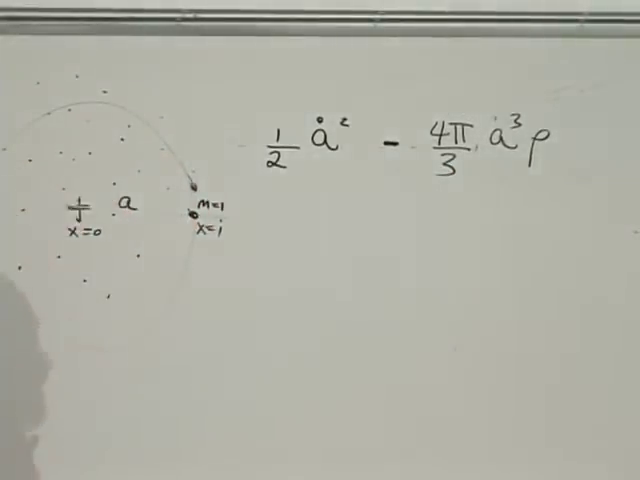
\includegraphics[width=0.78\textwidth]{lecture_03_figure_02.png}
\caption{\(x=0\)을 중심으로 한 균일한 구, \(x=1\)에 있는 공변 은하, 그리고 \(a(t)\)에 대한 뉴턴 역학적 에너지 균형.}
\end{figure}

반지름이 \(a(t)\)인 구 안의 물질만이 \(x=1\)에 있는 입자에 중력을 가한다. 이 입자의 질량을 단위 질량으로 두면 운동 에너지는 다음과 같다.
\begin{equation}
\frac{1}{2}\dot a^2.
\end{equation}
구 안에 포함된 질량은
\begin{equation}
M_{\mathrm{enc}}=\frac{4\pi}{3}a^3\rho,
\end{equation}
이므로 중력 위치 에너지는
\begin{equation}
-\frac{G M_{\mathrm{enc}}}{a}
=
-\frac{4\pi G}{3}a^2\rho.
\end{equation}
\editorialnote{강의 시각 00:05:30에 판에는 운동 항과 밀도에 의존하는 위치 에너지 항이 명확히 적혀 있다. 여기에 적힌 전체 계수는 강의에서 구두로 설명한 유도에 따른다.}

에너지 보존에 따라
\begin{equation}
\frac{1}{2}\dot a^2-\frac{4\pi G}{3}a^2\rho=\text{const}.
\end{equation}
상수는 \(-k\)로 표기한다. 다만 통상적인 정규화에서는 방정식에 \(2\)를 곱한 뒤에야 이 표기가 정해진다는 점에 유의해야 한다. 표준형은
\begin{equation}
\dot a^2=\frac{8\pi G}{3}a^2\rho-k,
\end{equation}
이고, \(a^2\)로 나누면
\begin{equation}
\left(\frac{\dot a}{a}\right)^2=\frac{8\pi G}{3}\rho-\frac{k}{a^2}.
\end{equation}
이 된다. 이것이 여기서 논의하는 동안 사용하는 형태의 프리드만 방정식이다.

\begin{figure}[ht]
\centering
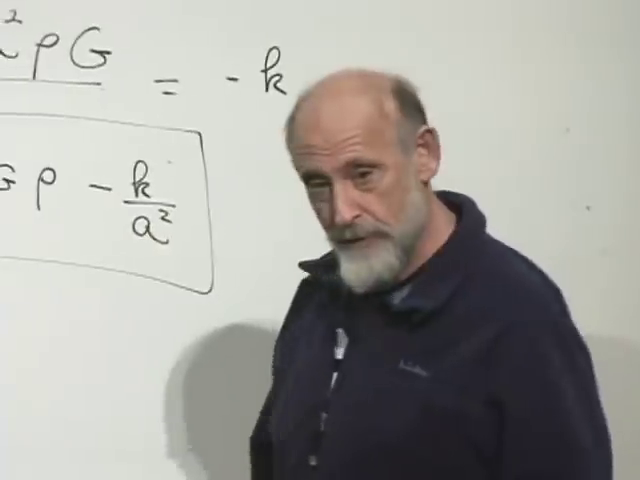
\includegraphics[width=0.56\textwidth]{lecture_03_figure_03.png}
\caption{프리드만 방정식에서 분리해 나타낸 곡률 항 \(-k/a^2\).}
\end{figure}

곡률 항은 관측상 0에 매우 가깝기 때문에, 이 수준에서는 무시해도 아주 좋은 근사가 된다. 이 항은 공간의 곡률에 해당하지만, 관측값이 너무 작아 여기서는 곡률의 부호조차 정할 수 없다.

같은 방정식은 일반 상대성 이론에서도 얻어진다. 시간-시간 성분의 아인슈타인 방정식을 개략적으로 쓰면
\begin{equation}
R_{00}-\frac{1}{2}g_{00}R \propto T_{00}.
\end{equation}
\editorialnote{여기서는 정확한 전체 수치 계수가 아니라 텐서 구조만 제시한다.}
팽창하는 균일한 계량을 쓰면 기하학적 측에서는 \(\dot a/a\)와 \(k/a^2\)의 조합이 나오고, 물질 측에서는 에너지 밀도가 나온다. 이 단계에서는 뉴턴 역학적 논증과 아인슈타인 방정식이 같은 내용을 말한다.

이로 인해 \(\rho\)의 의미도 달라진다. 이제부터는 \(\rho\)를 에너지 밀도라고 부르는 편이 낫다. 공변 좌표계에서 느리게 움직이는 물질의 경우, 이는 곧 정지 에너지 밀도다.

\section{물질 우세 시대}

이제 에너지 밀도가 공변 좌표계에서 정지해 있는 물질에 실려 있다고 가정하자. 한 변이 좌표 단위 길이인 정육면체를 생각한다. 각 변의 물리적 길이는 \(a(t)\)이므로 물리적 부피는 \(a^3(t)\)이다. 이 공변 정육면체 안의 질량-에너지가 \(M\)이고, 물질이 흐름을 따라 움직여 경계를 넘지 않는다면
\begin{equation}
\rho_m=\frac{M}{a^3}.
\end{equation}

이것이 물질 우세 경우다. 이 이상화에서는 입자들이 상자 안에서 정지해 있으므로 온도와 압력을 모두 0으로 둔다. 압력이 있으려면 입자들이 상자의 경계를 통과해야 한다.

\(k\approx 0\)이면 방정식은
\begin{equation}
\left(\frac{\dot a}{a}\right)^2=\frac{8\pi G}{3}\frac{M}{a^3}.
\end{equation}
이 된다. 거듭제곱 꼴을 가정해 보자.
\begin{equation}
a(t)=Ct^p.
\end{equation}
그러면
\begin{equation}
\frac{\dot a}{a}=\frac{p}{t},
\end{equation}
이므로 좌변은 \(t^{-2}\)에 비례하고 우변은 \(t^{-3p}\)에 비례한다. 거듭제곱을 맞추면
\begin{equation}
3p=2,
\qquad
p=\frac{2}{3}.
\end{equation}
을 얻는다. 따라서
\begin{equation}
a(t)\propto t^{2/3}.
\end{equation}
이고, 계수까지 유지하면
\begin{equation}
C^3=6\pi G M.
\end{equation}

해의 핵심은 거듭제곱 법칙이다. 물질이 지배하는 우주는 시간에 선형적으로 비례해 팽창하는 것이 아니라 시간의 3분의 2제곱에 비례해 팽창한다. 이 법칙은 빅뱅 후 대략 \(10^5\)년부터 몇십억 년 뒤까지 이어지는 긴 중간 시대를 설명한다. 현재 우주는 문자 그대로 물질이 지배하는 상태가 아니다. 지금은 암흑 에너지가 지배적이기 때문이다. 그러나 보통 물질과 우주 역사의 상당 기간은 이 법칙으로 설명된다.

\section{복사 우세 시대}

그보다 이른 시기에는 에너지 밀도에서 복사가 우세했다. 이유는 간단하다. 우주에는 엄청난 수의 광자가 있어 양성자 하나당 대략 \(10^9\)개의 광자가 존재하며, 우주가 압축되면 이 광자들의 에너지가 커진다.

광자에는 정지 질량이 없지만 에너지는 있다. 광자의 에너지는
\begin{equation}
E_\gamma=h\nu=\frac{hc}{\lambda}.
\end{equation}
이다. 핵심 가정은 우주가 팽창할 때 광자의 파장도 함께 늘어난다는 것이다.
\begin{equation}
\lambda\propto a.
\end{equation}
상자 안의 파동을 떠올리면 이해하기 쉽다. 상자가 커지면 그 안의 모드의 파장도 상자와 함께 늘어난다. 여기서는 팽창하는 우주에 같은 생각을 적용한다.

\(\lambda\propto a\)이므로 각 광자의 에너지는
\begin{equation}
E_\gamma\propto a^{-1}.
\end{equation}
에 비례한다. 다시 공변 단위 상자를 생각하자. 광자들은 드나들지만, 상자 안의 광자 수는 평균적으로 일정하다. 그러면 상자 안의 전체 광자 에너지도 \(a^{-1}\)에 비례한다. 이를 물리적 부피 \(a^3\)로 나누면 복사 에너지 밀도는
\begin{equation}
\rho_r\propto a^{-4}.
\end{equation}
에 비례한다.

이 추가적인 \(a^{-1}\) 인자가 차이를 만든다. 물질은 우주가 팽창하기 때문에 희석된다. 복사는 그 이유로 희석될 뿐 아니라 각 광자의 적색편이 때문에 에너지도 줄어든다.

따라서 복사 우세 우주에 대한 프리드만 방정식은
\begin{equation}
\left(\frac{\dot a}{a}\right)^2=\frac{8\pi G}{3}\frac{M_r}{a^4}.
\end{equation}
이다. \editorialnote{강의에서는 이 새로운 상수에도 기호 \(M\)를 다시 사용한다. 여기서는 물질의 경우와 혼동하지 않도록 아래 첨자 \(r\)만 덧붙였다.}

같은 시도 함수 \(a(t)=Ct^p\)를 사용하자. 좌변은 다시 \(t^{-2}\)에 비례하고, 우변은 \(t^{-4p}\)에 비례한다. 거듭제곱을 맞추면
\begin{equation}
4p=2,
\qquad
p=\frac{1}{2}.
\end{equation}
을 얻는다. 따라서
\begin{equation}
a(t)\propto t^{1/2}.
\end{equation}
이고, 계수까지 유지하면
\begin{equation}
C^4=\frac{32\pi G}{3}M_r.
\end{equation}

\begin{classroomqa}
\lecturetimestamp{00:35:41}
\audiencequestion{여기에 \(G\)가 들어가는 이유가 뭔가요?}
\lecturerresponse{중력을 만드는 것은 정지 질량만이 아니라 에너지 밀도이기 때문입니다. 느리게 움직이는 물질에서는 그 차이를 알아차리기 어렵지만, 광자를 보면 분명해집니다. 광자는 정지 질량이 없는데도 중력을 만듭니다.}
\end{classroomqa}

복사로 가득 찬 상자를 생각하면 요점이 분명해진다. 광자가 들어 있는 상자를 밀어 보자. 상자가 가속하기 시작하면 광자 쪽으로 움직이는 벽은 광자에게서 멀어지는 벽보다 더 강한 충격을 받으므로, 복사압에 맞서 더 큰 힘으로 밀어야 한다. 따라서 상자는 추가 관성을 갖고, 등가 원리에 따르면 이 추가 관성은 추가 중력 질량도 의미한다. 에너지가 중력을 만든다고 설명할 때 여기서 사용하는 것이 바로 이 광자 상자 논증이다.

\begin{classroomqa}
\lecturetimestamp{00:38:11}
\audiencequestion{시간이 지나면서 감소하는 \(a\)를 갖는 해가 이 방정식들 중 하나라도 있나요?}
\lecturerresponse{있습니다. 곡률 항 \(k/a^2\)을 되살리면 팽창했다가 수축하는 해가 존재합니다. 우리 우주는 그렇게 움직이는 것처럼 보이지 않지만, 방정식은 그런 해를 허용합니다.}
\end{classroomqa}

\begin{classroomqa}
\lecturetimestamp{00:38:44}
\audiencequestion{에너지 보존은 어떻게 된 건가요?}
\lecturerresponse{\(k\) 항을 되살리고 방정식에 다시 \(a^2\)을 곱하면, 우주론 방정식은 정확히 보존 법칙이 됩니다. 한쪽에 있는 물질이나 복사는 장부에 기록되는 항의 일부일 뿐입니다. 팽창은 운동 에너지와 중력 에너지 항을 보태며, 전체 에너지 균형은 보존됩니다.}
\end{classroomqa}

\section{물질과 복사의 공존}

실제 우주론에서는 물질과 복사가 모두 존재한다. 두 성분의 밀도는 서로 다르게 변한다.
\begin{equation}
\rho_m\propto a^{-3},
\qquad
\rho_r\propto a^{-4}.
\end{equation}
따라서 \(a\)가 작을 때는 복사가 우세하고, \(a\)가 클 때는 물질이 우세하다. 시간을 거슬러 올라가면 초기 우주는 복사 우세였음이 틀림없다.

\begin{figure}[ht]
\centering
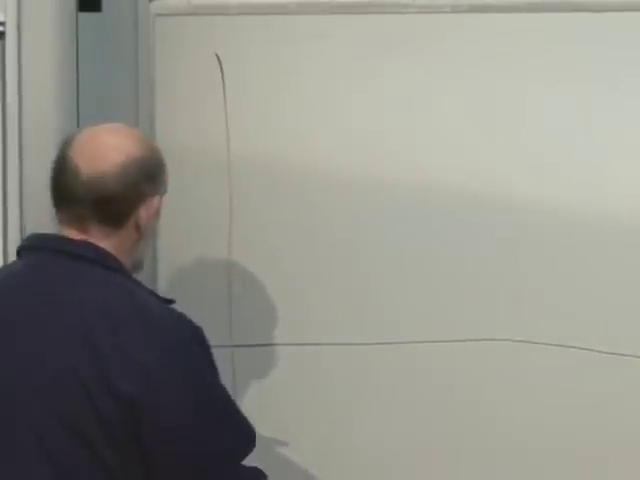
\includegraphics[width=0.68\textwidth]{lecture_03_figure_05.png}
\caption{척도 인자의 함수로서 물질과 복사의 에너지 밀도를 비교하기 위한 축.}
\end{figure}

\editorialnote{강의 시각 00:44:45에 판에는 비교 그래프의 축만 처음으로 나타난다. 바로 뒤에서 논의하는 물질 곡선과 복사 곡선은 다시 그리지 않고 본문에서 설명한다.}

물질 곡선은 \(a^{-3}\)에 따라 감소하고, 복사 곡선은 \(a^{-4}\)에 따라 감소한다. 두 곡선 모두 \(a\to 0\)일 때 발산하지만, 그 지점에서 복사 곡선이 더 빠르게 증가하므로 두 곡선은 등가 척도 인자에서 교차한다. 대략적인 추정에 따르면 이 전이는 약 \(10^4\)년 뒤에 일어나며, 실제로는 조금 더 늦을 수도 있다.

같은 내용을 \(a(t)\)를 \(t\)의 함수로 나타낸 그래프에서도 볼 수 있다. 초기에는 팽창이 \(t^{1/2}\)처럼 진행되고, 나중에는 \(t^{2/3}\)처럼 진행된다. 변화는 갑작스럽게 일어나지 않고, 비교적 좁은 시간 범위에 걸쳐 연속적으로 교차한다.

\begin{classroomqa}
\lecturetimestamp{00:44:04}
\audiencequestion{우주가 나이를 먹으면서 거듭제곱 \(p\)가 \(1/2\)에서 \(2/3\)로 연속적으로 변하나요?}
\lecturerresponse{그렇습니다. 갑자기 바뀌지는 않습니다. 꽤 좁은 시간 범위에서 일어나기는 하지만 변화는 연속적입니다.}
\end{classroomqa}

\section{온도, 재결합, 최종 산란}

다음으로 살펴볼 양은 온도다. 전형적인 광자의 에너지가 \(a^{-1}\)에 비례한다면, 복사 열욕의 온도도 마찬가지다.
\begin{equation}
T\propto a^{-1}.
\end{equation}
\(a\)가 두 배가 되면 온도는 절반으로 낮아진다.

현재 광자 온도를 약 \(3\,\mathrm K\), 이온화 온도를 약 \(3000\,\mathrm K\)로 두자. 후자는 대략 태양 표면의 온도다. 그러면
\begin{equation}
\frac{a_{\mathrm{today}}}{a_{\mathrm{ion}}}\sim 10^3.
\end{equation}
후기 물질 우세 시대의 법칙 \(a\propto t^{2/3}\)을 사용하면
\begin{equation}
\left(\frac{t_{\mathrm{today}}}{t_{\mathrm{ion}}}\right)^{2/3}\sim 10^3,
\end{equation}
이므로
\begin{equation}
\frac{t_{\mathrm{today}}}{t_{\mathrm{ion}}}\sim 1000^{3/2}\sim 3\times 10^4.
\end{equation}
이 추정의 정확도에서 우주의 나이를 \(10^{10}\)년으로 두면
\begin{equation}
t_{\mathrm{ion}}\sim 3\times 10^5\ \mathrm{years}.
\end{equation}

이 시기에 수소와 헬륨은 더 이상 완전히 이온화된 상태를 유지하지 않는다. 그보다 이른 우주는 뜨거운 플라스마다. 플라스마는 왜 불투명할까? 자유 전하가 전자기파에 강하게 반응하기 때문이다. 전기장이 전하를 앞뒤로 움직이고, 매질은 도체처럼 거동하며, 도체는 불투명하다. 이것이 태양 표면과 관련된 비유다.

우주가 충분히 식어 전자가 원자핵과 재결합하면 보통의 중성 원자가 형성되고 우주는 훨씬 투명해진다. 이 전이는 무한히 날카롭지는 않다. 어느 정도 퍼진 구간, 즉 흐릿한 시간 범위에 걸쳐 일어나지만, 우주론에서 다루기에는 충분히 뚜렷하므로 최종 산란면이라고 부른다.

바깥을 본다는 것은 시간을 거슬러 본다는 뜻이다. 가까운 은하에서는 최근 과거를 보고, 더 먼 은하에서는 더 이른 시기를 본다. 충분히 멀리 보면 모든 시선이 우주가 아직 이온화되어 불투명했던 시기에 이른다. 전자기 복사로는 그보다 더 이른 시기를 볼 수 없다.

원리적으로는 다른 메신저 입자들로 더 이른 시기를 탐사할 수 있다. 중성미자는 전기적으로 중성이므로 더 이른 시기에 열적 평형에서 분리되었을 것이다. 중력자는 관측할 수만 있다면 그보다 더 이른 시대에서 왔을 것이다. 그러나 초기 플라스마를 통과하게 해 주는 약한 상호작용 때문에 이 입자들은 검출하기도 매우 어렵다.

우주가 한때 모든 방향에서 태양 표면만큼 뜨거웠다면, 하늘은 왜 눈부시게 밝지 않을까? 최종 산란면이 멀어지고 있고, 거기서 도착하는 광자들이 \(10^3\) 정도의 비율만큼 적색편이되었기 때문이다. 이는 \(3000\,\mathrm K\)와 \(3\,\mathrm K\) 사이의 비율과 대략 같다. 우리에게 도달하는 것은 가시광선이 아니라 마이크로파 복사다.

\begin{classroomqa}
\lecturetimestamp{01:03:51}
\audiencequestion{그러면 우리 망원경으로는 약 \(300{,}000\)년보다 더 이른 시기를 볼 수 없나요?}
\lecturerresponse{전자기파 망원경으로는 볼 수 없습니다. 그 시기 이전의 우주는 이온화되어 불투명했습니다. 원리적으로는 다른 메신저 입자들로 더 이른 시대를 탐사할 수 있습니다.}
\end{classroomqa}

\begin{classroomqa}
\lecturetimestamp{01:08:43}
\audiencequestion{광자의 온도라고 할 때는 그 광자의 최고 복사에 해당하는 흑체의 온도를 뜻하는 거죠. 그런데 그 온도는 파장에 선형적으로 비례하지 않죠?}
\lecturerresponse{맞습니다. 온도는 본질적으로 전형적인 광자의 에너지이므로, 광자의 경우 파장에 반비례합니다. \(T^4\) 법칙은 개별 광자의 에너지가 아니라 에너지 밀도를 가리킵니다. 이 법칙은 광자 하나당 에너지와 단위 부피당 광자 수를 결합하며, 수밀도는 \(T^3\)에 비례합니다.}
\end{classroomqa}

따라서
\begin{equation}
n_\gamma\propto T^3,
\qquad
\rho_\gamma\propto T^4.
\end{equation}

\section{회전 곡선으로 알아보는 암흑 물질}

암흑 물질은 은하 회전 곡선을 통해 등장한다. 이는 대규모 프리드만 방정식에서 추론된 것이 아니라 은하 규모의 천문 관측에서 추론되었다.

가장 단순한 뉴턴 역학 문제부터 시작하자. 질량 \(m\)인 가벼운 물체가 중심 질량 \(M\)을 반지름 \(r\)인 궤도로 돈다고 하자. 중력은
\begin{equation}
\frac{GMm}{r^2},
\end{equation}
이고 구심 가속도는 \(v^2/r\)이다. 뉴턴 법칙에 따르면
\begin{equation}
m\frac{v^2}{r}=\frac{GMm}{r^2}.
\end{equation}
이다. \(m\)를 약분하고 \(r\)를 곱하면
\begin{equation}
v(r)=\sqrt{\frac{GM}{r}}.
\end{equation}
을 얻는다. 따라서 중력을 만드는 질량이 중심 부근에 집중되어 있다면 공전 속도는 \(r^{-1/2}\)에 따라 감소한다.

질량이 빛을 따라 분포한다면 이렇게 예상할 수 있다. 은하에서 보이는 물질 대부분은 중심핵 부근에 있으므로 바깥쪽 별들은 태양계 바깥 행성들과 비슷하게 움직일 것이다. 천문학자들은 가까운 은하의 양쪽에서 도플러 편이 차이를 측정해 공전 속도를 추론한다. 이때 은하 전체의 후퇴 운동을 먼저 빼고, 우리 쪽으로 다가오는 쪽과 멀어지는 쪽을 비교한다. 측정된 공전 속도는 큰 반지름까지 대체로 일정하게 유지된다.

그러므로 중심 질량 \(M\) 대신 반지름 안에 포함된 질량 \(M(r)\)를 넣으면
\begin{equation}
\frac{v^2}{r}=\frac{G M(r)}{r^2}.
\end{equation}
이 된다. \(v(r)\)가 대략 일정하다면
\begin{equation}
M(r)\propto r.
\end{equation}
이다. 다시 말해, 보이는 빛이 더는 증가하지 않는 곳에서도 중력을 만드는 질량은 반지름에 따라 계속 증가한다.

이제 논의에서 단순화를 위해 가정하듯 질량 분포가 대략 구형이라고 하자. 그러면
\begin{equation}
M(R)=\int_0^R 4\pi r^2\rho(r)\,dr.
\end{equation}
이다. \(M(R)\propto R\)라면 \(R\)에 대해 미분하여
\begin{equation}
4\pi R^2\rho(R)\propto 1,
\end{equation}
을 얻으며, 따라서
\begin{equation}
\rho(r)\propto \frac{1}{r^2}.
\end{equation}

\begin{classroomqa}
\lecturetimestamp{01:28:18}
\audiencequestion{밀도가 \(1/r^2\)에 비례할 것 같은데, 그 이유가 있나요?}
\lecturerresponse{관측된 평탄한 회전 곡선으로부터 \(M(R)\propto R\)를 추론하고, 이를 미분하면 \(\rho(r)\propto 1/r^2\)을 얻습니다. 그 이상으로는 여기서 간단한 제일 원리 설명을 주장하지 않습니다. 상세한 시뮬레이션이 많은 부분을 담당합니다.}
\end{classroomqa}

확실한 결론은 은하에 발광 물질만으로 예상되는 것보다 훨씬 많은 중력 질량이 있다는 점이다. 그 질량은 몇 배가량 더 많으며, 여기서 사용한 추정치로는 대략 한 자릿수 정도 더 많다. 보이는 은하는 훨씬 큰 암흑 헤일로 안에 놓여 있다.

보통의 기체는 어떻게 그렇게 희박한 상태에 머무르지 않을까? 소산 때문이다. 충돌과 마찰 같은 과정, 그리고 복사로 에너지를 잃을 수 있기 때문에 기체 구름은 수축한다. 암흑 물질은 유의미한 복사를 하지 않고 거의 충돌하지 않는 것으로 보인다. 중력은 암흑 물질을 안쪽으로 끌어당겨 위치 에너지를 운동 에너지로 바꿀 수 있지만, 효율적인 소산이 없으면 보통 물질이 만드는 작고 밝은 구조로 붕괴하지 않는다. 헤일로를 확장된 상태로 유지하는 것은 운동 에너지다.

이어서 몇 가지 대안이 신중하게 논의된다. 중성미자는 은하 규모에서 이런 식으로 거동하기에는 너무 빠르다고 한다. 보통의 수소로 이루어진 헤일로는 초기 우주의 핵합성을 크게 교란할 것이다. 보통의 물질로 이루어진 블랙홀도 문제가 될 수 있다고 언급한다. 초기 우주에 보통 물질이 너무 많다는 뜻이 되고 중력 렌즈 효과와 관련된 문제도 일으킬 수 있기 때문이다. 강의에서는 그 자리에서 이 이상의 주장을 하지는 않는다.

헤일로는 얇은 껍질이나 토러스 형태로 묘사되지 않는다. 중심부가 더 조밀하고 바깥쪽으로 갈수록 점진적으로 희박해지는, 대략 구형의 불균일한 덩어리다.

\begin{classroomqa}
\lecturetimestamp{01:53:12}
\audiencequestion{불릿 성단을 말씀하시는 건가요?}
\lecturerresponse{그렇습니다. X선 기체는 보통 물질을 보여 주고, 중력 렌즈 효과는 중력을 만드는 전체 질량을 보여 줍니다. 충돌 과정에서 두 분포는 서로 분리됩니다. 이는 보이는 물질에만 작용하는 단순한 중력 수정이 아니라 실제 암흑 물질이 존재한다는 강력한 증거입니다.}
\end{classroomqa}

이것이 마지막 관측상의 요점이다. 암흑 물질이 무엇인지에 관해 구체적으로 알려진 것은 거의 없지만, 여기서 급진적인 새 원리를 가정할 필요는 없다. 보수적으로 생각하면 자연에는 아직 확인되지 않은, 약하게 상호작용하는 입자들이 추가로 존재한다고 보면 된다.

\chapter{지평선, 상태방정식, 진공 에너지}

\section{선호 기준계, 초광속 후퇴, 지평선}

우주 마이크로파 배경복사는 실제로 특별한 기준계를 정해 준다. 이 복사가 등방적으로 보이는 기준계에서는 가까운 은하들도 평균적으로 정지해 있다. 우리가 배경복사에 대해 움직이면 진행 방향의 광자는 도플러 효과로 에너지가 높아지고, 반대 방향의 광자는 에너지가 낮아진다. 선호 기준계는 마이크로파 배경복사가 등방적으로 보이는 기준계이며, 평균적으로 국소 은하들이 정지해 있는 기준계이기도 하다.

\begin{classroomqa}
\lecturetimestamp{00:00:25}
\audiencequestion{우주 복사의 겉보기 파장은 관측자의 운동에 따라 달라지나요? 그렇다면 선호 기준계가 있다는 뜻인가요?}
\lecturerresponse{그렇습니다. 마이크로파 배경복사에 대해 움직이면 도플러 비등방성이 생기므로 우주론적 선호 기준계가 있습니다. 마이크로파 배경복사가 등방적으로 보이는 기준계가 바로 그것입니다. 이 기준계는 평균적으로 국소 은하들이 정지해 있는 기준계이기도 합니다.}
\end{classroomqa}

두 번째 질문은 후퇴 속도에 관한 것이다. 허블 법칙에 따르면 충분히 먼 은하들은 다음과 같은 속도로 서로 멀어진다.
\begin{equation}
v = H d .
\end{equation}
\(d\)가 충분히 크면 이 후퇴 속도는 빛의 속도를 넘는다. 이것은 상대성이론과 모순되지 않는다. 금지되는 것은 국소적인 상황, 즉 한 물체가 우리 바로 앞에서 다른 물체를 빛보다 빠르게 앞질러 가는 일이기 때문이다. 먼 은하들에 관한 진술은 서로 멀리 떨어진 장소들 사이의 기하에 관한 것이다.

\begin{classroomqa}
\lecturetimestamp{00:04:48}
\audiencequestion{두 은하 사이의 상대 속도가 \(c\)보다 클 수 있나요?}
\lecturerresponse{그렇습니다. 두 은하가 충분히 멀리 떨어져 있다면 가능합니다. 허블 후퇴 속도가 빛의 속도를 넘더라도 국소적 상대성이론을 위반하지 않습니다. 후퇴 속도가 \(c\)에 이르는 곳이 지평선입니다.}
\end{classroomqa}

후퇴 속도가 빛의 속도에 이르면 우리를 향해 보낸 신호는 더 이상 순수하게 우리 쪽으로 다가오지 못한다. 광선은 국소적으로 한계 속도로 움직이지만, 광선이 따라잡아야 할 거리가 너무 빠르게 늘어나기 때문이다.

\begin{classroomqa}
\lecturetimestamp{00:07:03}
\audiencequestion{반대 방향으로 보낸 광선은 그래도 우리 쪽으로 이동하지 않나요?}
\lecturerresponse{국소적으로는 그렇지만, 공간이 광선이 따라잡을 수 있는 속도보다 더 빠르게 팽창합니다. 광선은 가까운 점들에 대해 한계 속도로 움직이는 한편, 우리까지의 전체 거리는 계속 늘어납니다.}
\end{classroomqa}

\section{팽창하는 계량과 선의 비유}

1차원 그림을 생각하면 이해하기 쉽다. 원자들로 이루어진 선을 상상해 보자. 보통의 물질로 된 선을 잡아당기면 결국 끊어진다. 이제 그림을 조금 바꿔 보자. 이웃한 원자들이 너무 멀어질 때마다 그 사이에 원자를 하나씩 넣는다. 선은 계속 늘어나지만 국소적인 성질은 희박해지지 않는다.

\begin{figure}
\centering
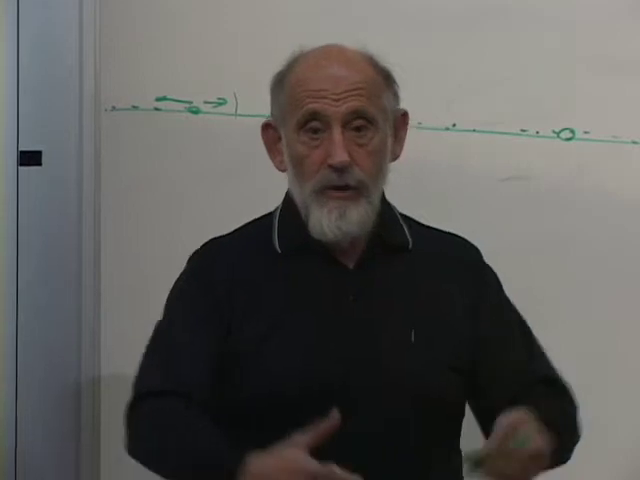
\includegraphics[width=0.60\textwidth]{lecture_04_figure_02.png}
\caption{팽창하는 계량을 나타내는 1차원 선의 비유.}
\end{figure}

이 그림에서도 국소적인 신호의 한계 속도는 여전히 존재한다. 보통의 선에서 소리가 한계 속도를 갖는 것과 같다. 규칙은 국소적이다. 교란은 가까운 점들에 대해 그 속도를 넘어설 수 없다. 그래도 선이 충분히 길고 새로운 점들이 충분히 빠르게 삽입되면, 충분히 멀리 떨어진 부분들은 신호가 끝내 돌아올 수 없을 만큼 빠르게 멀어진다.

따라서 특수상대론의 속도 합성 법칙은 이야기의 일부일 뿐이다. 이 법칙은 관측자들이 같은 지점에서 서로 지나칠 때 국소적으로 적용된다. 팽창하는 기하에서 멀리 떨어진 은하들을 다룰 때는 적절한 도구가 아니다.

\begin{classroomqa}
\lecturetimestamp{00:09:42}
\audiencequestion{이 상황에서도 보통의 상대론적 속도 합성 법칙이 성립하나요?}
\lecturerresponse{국소적으로, 한 지점에서는 그렇습니다. 관측자들이 차례로 서로를 지나친다면 보통의 특수상대론적 법칙이 적용됩니다. 하지만 \(c\)보다 빠른, 멀리 떨어진 천체들의 후퇴를 설명하는 데는 적절하지 않습니다. 그런 경우에는 팽창하는 공간의 기하를 살펴봐야 합니다.}
\end{classroomqa}

이 그림은 적색편이도 간단히 설명해 준다. 선 위에 파동을 그려 보자. 선이 팽창하면 파장도 함께 늘어난다. 팽창하는 기하에서는 이것이 단지 이해를 돕기 위한 비유에 그치지 않는다. 팽창하는 시공간의 파동 방정식은 실제로 늘어난 파장을 예측한다.

\begin{classroomqa}
\lecturetimestamp{00:14:42}
\audiencequestion{파동이 우주와 함께 늘어난다는 설명은 이론적인가요, 관측에 근거한 것인가요, 아니면 둘 다인가요?}
\lecturerresponse{팽창하는 시공간에서 파동이 전파될 때 이론적으로 따라 나오는 결과이며, 천문 관측으로도 뒷받침됩니다.}
\end{classroomqa}

이 그림은 고무줄과 다르다. 고무줄은 늘어나면 가늘어지고, 그런 매질 속에 사는 관측자는 국소적 성질이 변하는 것을 보게 된다. 여기서는 전역적인 거리 척도만 커질 뿐 국소적인 성질은 그대로 유지된다.

\section{최종 산란과 관측 가능한 우주}

지평선은 후퇴 속도가 빛의 속도에 이르는 곳이다. 최종 산란면은 그보다 약간 안쪽에 있다. 지평선에서 방출된 신호의 파장은 한없이 늘어나지만, 최종 산란 복사의 적색편이는 매우 크더라도 유한하다.

\begin{classroomqa}
\lecturetimestamp{00:17:53}
\audiencequestion{초광속 후퇴, 최종 산란면, 관측 가능한 우주는 어떤 관계인가요?}
\lecturerresponse{지평선은 후퇴 속도가 빛의 속도에 이르는 곳입니다. 최종 산란면은 적색편이가 엄청나게 크지만 유한하기 때문에 그보다 약간 안쪽에 있습니다. 실용적인 의미에서 최종 산란면은 관측 가능한 우주의 경계를 나타냅니다.}
\end{classroomqa}

최종 산란 복사의 적색편이는 대략 \(10^3\)배이다. 이 정도로도 최종 산란면은 여러 목적에서 지평선에 매우 가깝다. 관측 가능한 우주는 빛이 우리에게 도달할 수 있는 우주의 일부다.

후기에는 팽창이 진공 에너지 지배 영역에 가까워진다. 그러면 허블 매개변수는 일정한 값에 가까워지고, 지평선의 크기는 고정된 값에 가까워지며, 은하와 마이크로파 복사는 모두 점차 시야에서 사라진다.

\begin{classroomqa}
\lecturetimestamp{00:22:43}
\audiencequestion{\(H\)는 시간에 따라 변하는데, 지평선 거리는 변하나요? 마이크로파 배경복사는 결국 사라지나요?}
\lecturerresponse{후기에는 \(H\)가 일정한 값에 가까워지므로 지평선은 고정된 거리에 가까워집니다. 마이크로파 배경복사는 계속 늘어나고 식으면서 희미해집니다. 먼 은하들도 지평선을 지나 시야에서 사라집니다.}
\end{classroomqa}

이미 중력적으로 묶여 있는 구조만 시야에 남는다. 태양계는 흩어지지 않고 은하도 흩어지지 않지만, 큰 규모의 우주는 고립된 섬이 된다.

\section{기본 팽창 방정식과 세 성분}

이제 기본 팽창 방정식은 다음과 같다.
\begin{equation}
\left(\frac{\dot a}{a}\right)^2 = \frac{8\pi G}{3}\rho ,
\qquad c=1 .
\end{equation}
여기서 \(a(t)\)는 척도인자이고, \(\rho\)는 전체 에너지 밀도다.

\begin{figure}
\centering
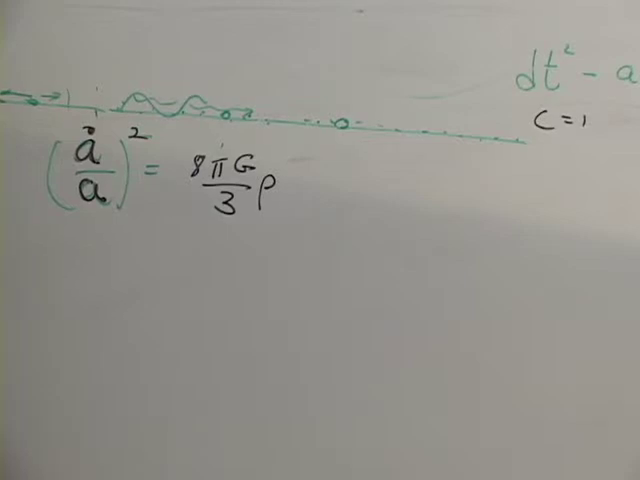
\includegraphics[width=0.74\textwidth]{lecture_04_figure_03.png}
\caption{기본 팽창 방정식과 1차원 선의 비유.}
\end{figure}

동역학적으로 중요한 성분은 세 가지다.

물질의 경우,
\begin{equation}
\rho=\frac{\text{const.}}{a^3},
\qquad
a(t)\sim t^{2/3}.
\end{equation}
이는 질량을 가진 물체들이 전체 팽창을 따라 움직이며 공변 기준계에서는 사실상 정지해 있는 경우다.

복사의 경우,
\begin{equation}
\rho=\frac{\text{const.}}{a^4},
\qquad
a(t)\sim t^{1/2}.
\end{equation}
\(a\)의 추가 거듭제곱은 우주가 팽창하면서 각 광자의 파장이 늘어나는 데서 비롯된다.

또한 다음 성분이 있다.
\begin{equation}
\rho_0=\text{constant},
\end{equation}
진공 에너지이며, 암흑 에너지라고도 하고 통상적인 수치 계수를 제외하면 우주 상수라고도 한다. 이 성분은 전혀 희석되지 않는다.

다음 단계는 에너지 밀도와 압력을 연결하는 것이다.

\section{복사 압력과 차가운 물질}

복사부터 살펴보자. 길이 \(L\)인 선분 하나만 있는 1차원 상자를 생각하자. 그 안에는 광자들이 앞뒤로 튕겨 다닌다. 1차원에서는 힘과 압력이 사실상 같은 양이다.

운동량 크기가 \(p\)인 광자를 생각하자. 광자가 벽에 반사될 때 운동량 변화는 다음과 같다.
\begin{equation}
\Delta p = 2p.
\end{equation}
같은 벽에 연속해서 충돌할 때까지의 시간은
\begin{equation}
\Delta t = \frac{2L}{c}.
\end{equation}
따라서 벽이 받는 평균 힘은
\begin{equation}
F=\frac{\Delta p}{\Delta t}=\frac{pc}{L}.
\end{equation}
광자의 경우,
\begin{equation}
E=pc,
\end{equation}
이므로
\begin{equation}
F=\frac{E}{L}.
\end{equation}
에너지를 길이로 나눈 값은 1차원 에너지 밀도다. 이 1차원 사례에서는
\begin{equation}
P=\rho .
\end{equation}

광자가 많더라도 평균을 취하면 같은 관계가 성립한다. 전체 힘은 단위 길이당 전체 에너지와 같다.

이제 3차원으로 가 보자. 모든 광자가 한 축을 따라서만 움직인다면 한 쌍의 면에는 압력을 가하지만 나머지 면에는 압력을 가하지 않는다. 일부러 틀린 가정이지만, 무엇을 바로잡아야 하는지는 바로 드러난다. 등방적인 복사에서는 운동량이 모든 방향으로 분포한다. 평균적으로 에너지 밀도의 3분의 1이 각 압력 성분에 기여한다. 따라서
\begin{equation}
P=\frac{\rho}{3}.
\end{equation}

차가운 물질의 경우에는 답이 다르다. 우주의 흐름을 따라 움직이는 작은 영역인 공변 상자를 생각하자. 안에 있는 입자들은 에너지를 갖고 있지만, 상자에 대해 정지해 있다면 벽에 부딪치지 않는다. 따라서 압력은
\begin{equation}
P=0.
\end{equation}

\begin{figure}
\centering
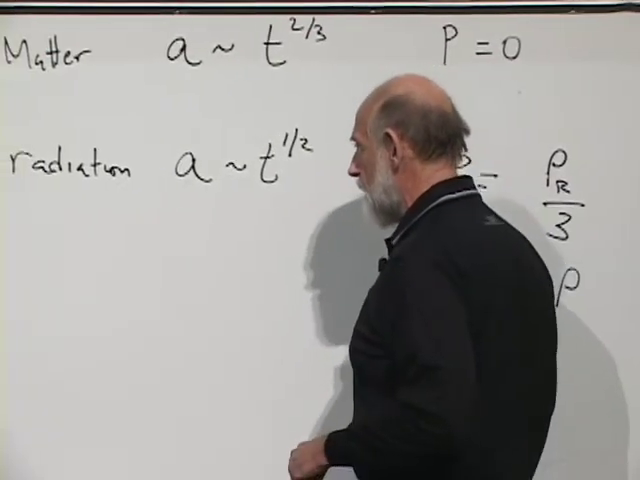
\includegraphics[width=0.74\textwidth]{lecture_04_figure_04.png}
\caption{물질과 복사: \(a\sim t^{2/3}\), \(P=0\), 그리고 \(a\sim t^{1/2}\), \(P=\rho/3\).}
\end{figure}

칠판의 요약은 다음과 같다.
\begin{align}
\text{matter:}\qquad & a(t)\sim t^{2/3}, \qquad P=0,\\
\text{radiation:}\qquad & a(t)\sim t^{1/2}, \qquad P=\frac{\rho}{3}.
\end{align}

\begin{classroomqa}
\lecturetimestamp{00:54:27}
\audiencequestion{팽창하는 우주에서 입자들이 실제로 서로 멀어지고 있지 않나요?}
\lecturerresponse{그렇습니다. 하지만 압력에 관한 논증은 무한소 크기의 공변 상자에 적용됩니다. 그 국소적인 규모에서는 열역학적 추론이 여전히 성립합니다.}
\end{classroomqa}

\section{상태방정식}

압력은 에너지 밀도에 비례한다고 둔다.
\begin{equation}
P=w\rho .
\end{equation}
칠판에서는 같은 매개변수를 \(\omega\)로 쓴다. 기본적인 두 경우는 다음과 같다.
\begin{equation}
w=0 \quad \text{for cold matter},
\qquad
w=\frac{1}{3} \quad \text{for radiation}.
\end{equation}

그 사이의 값도 가능하다. \(0\)와 \(1/3\) 사이의 값은 완전히 차갑지도 완전히 상대론적이지도 않은 물질을 나타낸다. 여기서 언급하는 예는 따뜻한 암흑 물질이다.

\begin{figure}
\centering
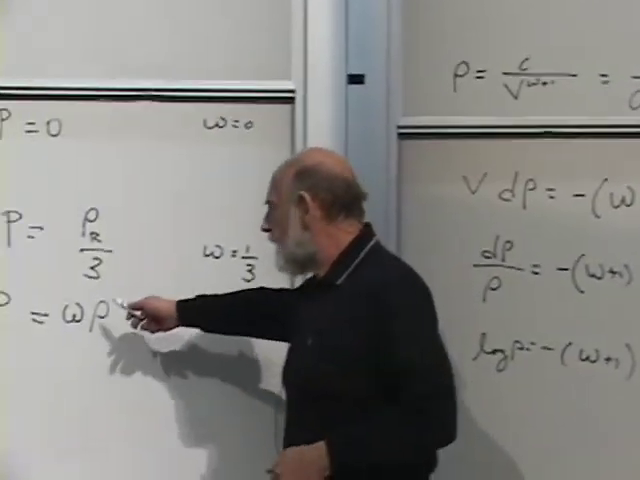
\includegraphics[width=0.74\textwidth]{lecture_04_figure_05.png}
\caption{상태방정식 \(P=\omega\rho\)과 밀도 스케일링 논증.}
\end{figure}

다음 질문은 \(w\)가 \(a\)에 따른 \(\rho\)의 변화를 결정하는가이다. 답은 열역학 항등식에서 나온다.

부피가 \(V\)인 상자를 생각하자. 내용물이 압력 \(P\)을 가할 때 상자가 \(dV\)만큼 팽창하면 벽에 한 일은 다음과 같다.
\begin{equation}
dE=-P\,dV.
\end{equation}
이제 에너지를 다음과 같이 쓰자.
\begin{equation}
E=\rho V.
\end{equation}
그 미분은
\begin{equation}
dE=\rho\,dV+V\,d\rho .
\end{equation}
두 식을 같게 놓으면
\begin{equation}
\rho\,dV+V\,d\rho=-P\,dV,
\end{equation}
또는
\begin{equation}
V\,d\rho=-(\rho+P)\,dV.
\end{equation}
\(P=w\rho\)를 사용하면,
\begin{equation}
V\,d\rho=-(1+w)\rho\,dV.
\end{equation}
\(\rho V\)로 나누면,
\begin{equation}
\frac{d\rho}{\rho}=-(1+w)\frac{dV}{V}.
\end{equation}
적분하면,
\begin{equation}
\rho \propto V^{-(1+w)}.
\end{equation}
공변 우주론적 상자에서는
\begin{equation}
V\propto a^3,
\end{equation}
따라서
\begin{equation}
\rho \propto a^{-3(1+w)}.
\end{equation}

앞서 본 경우들은 곧바로 얻어진다.
\begin{align}
w=0 &\Longrightarrow \rho \propto a^{-3},\\
w=\frac{1}{3} &\Longrightarrow \rho \propto a^{-4}.
\end{align}

이 때문에 \(w\)가 중요하다. \(\rho(a)\)를 알면 이를 프리드만 방정식에 대입할 수 있다. 그런 다음 거듭제곱 법칙 \(a\sim t^\alpha\)를 가정해 보고, 해당 상태방정식에서 우주가 어떻게 팽창하는지 구한다.

\section{진공 에너지와 음의 압력}

한 가지 특별한 경우는 다르게 거동한다.
\begin{equation}
w=-1.
\end{equation}
그러면
\begin{equation}
1+w=0,
\end{equation}
따라서 지수가 0이 되고,
\begin{equation}
\rho=\rho_0=\text{constant}.
\end{equation}
이에 해당하는 압력은
\begin{equation}
P=-\rho .
\end{equation}

음의 압력 자체가 신비로운 것은 아니다. 양의 압력은 상자의 벽을 바깥쪽으로 민다. 음의 압력은 안쪽으로 당긴다. 즉 장력이다. 늘어난 고무줄이 일상적인 예다. 고무줄은 양의 에너지를 저장하지만 양 끝을 서로 끌어당긴다.

일정한 밀도 \(\rho_0\)를 프리드만 방정식에 대입하면,
\begin{equation}
\left(\frac{\dot a}{a}\right)^2=\frac{8\pi G}{3}\rho_0.
\end{equation}
우변은 상수이므로
\begin{equation}
\frac{\dot a}{a}=\sqrt{\frac{8\pi G}{3}\rho_0}.
\end{equation}
허블 매개변수가 실제로 일정한 특별한 경우다. 방정식은 다음과 같이 쓸 수 있고,
\begin{equation}
\dot a=\sqrt{\frac{8\pi G}{3}\rho_0}\,a,
\end{equation}
해는 다음과 같다.
\begin{equation}
a(t)\propto \exp\!\left(\sqrt{\frac{8\pi G}{3}\rho_0}\,t\right).
\end{equation}

이는 지수 팽창이다. 관련된 시간 척도는 배가 시간이 아니라 \(e\)배 시간이므로, 여기서 사용하는 대략적인 추정에 따르면 우주의 나이와 비슷한 규모다. 진공 에너지와 우주 상수는 역사적인 수치 관례를 제외하면 같은 물리적 성분이다.

\begin{classroomqa}
\lecturetimestamp{01:27:16}
\audiencequestion{진공 에너지가 지수 팽창을 일으킨다면 결국 모든 것이 찢겨 나가지 않나요?}
\lecturerresponse{반드시 그렇지는 않습니다. 묶인 계는 팽창에 저항할 수 있습니다. 은하, 태양계, 원자는 반드시 찢겨 나가는 것이 아닙니다. 반면 충분히 크고 희박한 구조는 팽창에 참여해 결국 서로 멀어집니다.}
\end{classroomqa}

\begin{classroomqa}
\lecturetimestamp{01:31:43}
\audiencequestion{프리드만 방정식의 제곱근을 취할 때 나오는 음의 부호에도 흥미로운 의미가 있나요?}
\lecturerresponse{그렇습니다. 제곱근을 취하면 두 가지 해가 나옵니다. 하나는 팽창 해이고, 다른 하나는 시간 반전된 수축 해입니다. 방정식 자체는 둘 다 허용합니다.}
\end{classroomqa}

\section{세 시대와 관측된 팽창 역사}

세 성분이 모두 존재하며, 각각 다음과 같이 스케일링한다.
\begin{equation}
\begin{aligned}
\rho_{\text{radiation}}&\propto a^{-4},\\
\rho_{\text{matter}}&\propto a^{-3},\\
\rho_0&=\text{constant}.
\end{aligned}
\end{equation}
이로부터 세 시대가 바로 따라 나온다.

\(a\)가 매우 작을 때는 복사가 지배한다. 그 뒤에는 물질이 지배한다. \(a\)가 충분히 커지면 진공 에너지가 지배한다. 이에 해당하는 팽창 법칙은 다음과 같다.
\begin{equation}
a(t)\sim t^{1/2},
\qquad
a(t)\sim t^{2/3},
\qquad
a(t)\sim e^{Ht}.
\end{equation}

여기서 언급하는 대략적인 시점은 다음과 같다. 복사 지배 시대는 약 \(10^4\)년 뒤에 물질 지배 시대로 넘어간다. 우주가 투명해지는 것은 그보다 뒤인 약 \(10^5\)년 뒤다. 물질 지배에서 가속 팽창으로의 전이는 훨씬 나중에, 수십억 년이 지난 뒤 일어나며, 여기서 사용하는 자릿수 추정으로는 우주 역사의 대략 중간쯤이다.

이 역사를 어떻게 추론할까? 미래는 볼 수 없지만 과거는 볼 수 있다. 더 먼 곳을 바라보는 것은 더 이른 시점을 보는 일이다. 먼 은하들을 관측하고, 그 운동과 거리 사이의 관계를 측정하고, 되돌아보는 시간에 따른 허블 매개변수를 재구성하면 척도인자의 시간에 따른 역사를 알아낼 수 있다. 복사 지배 시대는 일반적인 은하 천문 관측으로 직접 볼 수 없을 만큼 이르지만, 물질 지배 시대와 진공 에너지 지배로의 전이는 재구성한 곡선에서 확인할 수 있다.

\section{아주 먼 미래의 최종 산란}

미래의 마이크로파 하늘은 은하들이 지평선을 넘어 사라지는 이야기와는 다르다. 나중에 우리가 보는 복사는 더 먼 곳의 물질에서 오므로, 같은 원자들이 그저 멀어지는 것을 지켜보는 것이 아니라 더 깊은 곳을 더 차갑게 보는 효과다.

\begin{classroomqa}
\lecturetimestamp{01:48:07}
\audiencequestion{최종 산란면이 지평선 속으로 희미해진다면, 이는 은하들이 지평선 너머로 움직이는 것과 같은 현상인가요?}
\lecturerresponse{아닙니다. 나중에 보이는 복사는 지금 우리가 보는 복사와 같은 원자들에서 오는 것이 아닙니다. 더 멀리 있던 원자들에서 오므로, 우주를 점점 더 깊이 들여다보는 것과 같습니다. 복사는 점점 더 차갑게 보입니다.}
\end{classroomqa}

\section{곡률, 빅 크런치 그림, 후기의 지평선}

지금까지는 곡률 항을 생략했다. 이를 다시 포함하면
\begin{equation}
\left(\frac{\dot a}{a}\right)^2
=
\frac{8\pi G}{3}\rho
-
\frac{K}{a^2}.
\end{equation}
수치상으로는 이 항이 작아 보이지만, 개념적으로는 중요하다. 오래된 뉴턴 역학의 표현으로는 전체 에너지가 양수인지, 0인지, 음수인지를 구분한다. 상대론적 표현으로는 공간의 기하를 구분한다.

진공 에너지를 진지하게 고려하기 전에는 물질 지배 우주에서 팽창이 결국 역전되리라고 흔히 생각했다. 그 결과가 오래된 빅 크런치 그림이다. 빅뱅으로 팽창을 시작한 뒤 다시 수축한다는 것이다. 그 수학은 여전히 유효하지만, 이제는 우리 우주를 설명하는 것처럼 보이지 않는다.

\begin{classroomqa}
\lecturetimestamp{01:53:51}
\audiencequestion{이 진공 에너지는 양자 진공 에너지와 관련이 있나요?}
\lecturerresponse{그렇습니다. 적어도 관련이 있다고 여겨집니다.}
\end{classroomqa}

현재의 대략적인 구성은 다음과 같다.
\begin{equation}
\frac{\rho_0}{\rho_{\text{total}}}\sim 0.7,
\qquad
\frac{\rho_{\text{matter}}}{\rho_{\text{total}}}\sim 0.3.
\end{equation}
물질 성분 가운데 발광 물질은 전체의 약 \(0.05\)이고 암흑 물질은 약 \(0.25\)이다. 현재 복사의 비중은 무시할 만하다. 암흑 물질과 발광 물질은 같은 방식으로 스케일링하므로, 물질·복사·진공 에너지의 상대적 비율이 시대마다 달라져도 둘 사이의 비율은 일정하게 유지된다.

진공 에너지가 지배하는 극한에서는
\begin{equation}
H=\sqrt{\frac{8\pi G}{3}\rho_0}.
\end{equation}
허블 법칙은 다음과 같이 된다.
\begin{equation}
v=Hd.
\end{equation}
지평선은 \(v=1\)로 정의되므로 그 거리는
\begin{equation}
d_H=\frac{1}{H}
=
\frac{1}{\sqrt{8\pi G\rho_0/3}}.
\end{equation}
여기서 제시하는 대략적인 값은 \(10\)에서 \(12\)십억 광년이다.

중요한 점은 후기의 거동이다. 팽창이 지수적으로 이루어지기 시작하면 지평선 거리는 고정된다. 은하들은 계속 지평선을 지나 적색편이가 점점 커지면서 시야에서 사라진다. 마이크로파 배경복사도 적색편이되어 사라진다. 먼 미래에는 가까운 중력 결합 구조만 시야에 남고, 우주는 고립된 섬처럼 보인다.

\section{최종 산란면으로 기하를 알아내기}

마지막으로 최종 산란면을 이용해 기하를 검증할 수 있다. 그 면까지의 거리를 안다고 하자. 그곳에서 물리적 크기를 충분히 정확히 아는 덩어리를 식별할 수 있다고도 하자. 그러면 그 크기와 거리를 관측된 각크기와 비교할 수 있다.

평탄한 공간에서는 각도가 유클리드 기하에서 예상하는 값이다. 양의 곡률을 가진 공간에서는 더 크게 보이고, 음의 곡률을 가진 공간에서는 더 작게 보인다. 일반적인 측량과 같은 비유다. 크기와 거리를 아는 물체를 두고 측정한 각도를 유클리드 기하의 예측과 비교한다.

\begin{classroomqa}
\lecturetimestamp{02:08:09}
\audiencequestion{저 멀리 있는 물체 가운데 크기를 아는 예가 있나요?}
\lecturerresponse{마이크로파 배경복사에서 가장 큰 덩어리들입니다. 진화에 걸린 시간과 음속을 바탕으로 그 크기를 안다고 생각합니다.}
\end{classroomqa}

여기서 중요한 물체는 마이크로파 배경복사에서 가장 큰 덩어리들이다. 관측된 각크기는 몇 퍼센트 이내에서 유클리드 기하와 일치한다. 이를 근거로 공간은 평탄해 보인다.

\section{측정된 \(w\)와 마지막 질문}

\(w\)의 관측상 중요성은 이제 분명하다. 천문학자들이 \(w\)가 \(-1\)에 매우 가깝다고 보고한다면, 진공 에너지 성분이 거의 일정하다는 뜻이다. 바로 이것이 여기서 말하는 요점이다.

그렇다고 일반상대성이론이 \(w\)가 정확히 \(-1\)여야 한다고 강제하는 것은 아니다. 여기서 요점은 경험적이다. 강의에서는 더 급진적인 가능성도 원칙적으로 배제되지 않는다고 짧게 언급하지만, 거의 일정한 진공 에너지의 경우가 그럴 만한 근거가 충분히 있는 경우다.

\begin{classroomqa}
\lecturetimestamp{02:11:04}
\audiencequestion{물질과 복사의 밀도를 계산할 때 에너지가 일정하다고 가정한 뒤, 식을 구하려고 척도인자를 조정했나요? 처음 두 경우에 그렇게 했다면 밀도가 일정하게 유지되는 진공 에너지의 경우에는 어떻게 되나요?}
\lecturerresponse{아닙니다. 에너지가 일정하다고 가정하지 않았습니다. 에너지 변화가 \(-P\,dV\)임을 사용했습니다. 팽창을 따라 움직이는 가상의 공변 상자를 생각하면, 벽에 일이 가해지고 그 결과 에너지가 변합니다. 진공 에너지의 경우에는 질문이 다른 방식으로 제기됩니다. 마지막으로 덧붙일 점은 우주론에서 에너지 보존이라는 표현이 그다지 많은 것을 말해 주지 않는다는 것입니다. 우주의 전체 에너지가 0이기 때문입니다.}
\end{classroomqa}
\chapter{구면, 쌍곡 공간, 그리고 \(k\)의 의미}

간단한 수학을 조금 해 봅시다. 차원이 몇이든 구는 특별한 기하학적 대상입니다. 구는 균일하며, 여기서 균일하다는 것은 곡률이 일정하다는 뜻입니다. 먼저 양의 곡률을 살펴보고, 이어서 균일한 음의 곡률을 본 다음 아인슈타인 방정식과의 연관성을 알아보겠습니다.

구형 우주란 \emph{공간}이 구형이라는 뜻이지, 시공간이 구형이라는 뜻은 아닙니다. 또 다른 가능성은 균일한 음의 곡률을 가진 경우입니다. 이 두 경우를 나란히 놓고 보면 일반 상대성이론의 역할이 분명해집니다.

\section{구와 균일한 기하학}

1차원 구는 단순히 원입니다. 이를 기술하는 가장 간단한 방법은 2차원 보조 공간에 매장하고 다음과 같이 쓰는 것입니다.
\begin{equation}
x^2+y^2=R^2.
\end{equation}
단위 1차원 구는 다음과 같습니다.
\begin{equation}
x^2+y^2=1.
\end{equation}

2차원 구도 같은 방식으로 기술하되, 이번에는 보조 좌표를 세 개 사용합니다.
\begin{equation}
x^2+y^2+z^2=R^2,
\end{equation}
단위 구의 경우에는 다음과 같습니다.
\begin{equation}
x^2+y^2+z^2=1.
\end{equation}

이 좌표들은 어디까지나 편의를 위한 보조 수단입니다. 관심 있는 기하학적 대상은 주변의 \(x,y,z\)공간이 아니라 표면 자체입니다. 1차원 구 위에 사는 생명체는 원 위에 살며, 안쪽이나 바깥쪽에 접근할 수 없습니다. 2차원 구에도 같은 생각을 적용할 수 있습니다. 구의 내부를 채우는 부분과 구 바깥은 보조적인 그림에만 속합니다.

같은 구성을 통해 3차원 구도 얻을 수 있습니다. 이를테면 \(w\)이라는 좌표를 하나 더 도입해 다음과 같이 씁니다.
\begin{equation}
x^2+y^2+z^2+w^2=R^2,
\end{equation}
단위 구의 경우에는 다음과 같습니다.
\begin{equation}
x^2+y^2+z^2+w^2=1.
\end{equation}
3차원 구는 시각화하기가 더 어렵습니다. 보조 공간이 4차원이 되기 때문입니다. 하지만 수학은 그리 더 어려워지지 않습니다.

표준 표기는 \(\Omega_n\)이며, \(n\)-구면에 대해 사용한다. 따라서 \(\Omega_1\)은 1-구면, \(\Omega_2\)은 2-구면, \(\Omega_3\)은 3-구면이다.

\section{구 위의 계량}

더 유용한 기술 방법은 내재적인 방식입니다. 구 자체에 놓인 좌표를 사용해 구를 기술합니다.

단위 1차원 구는 좌표 \(\phi\) 하나면 충분하며, \(0\leq \phi \leq 2\pi\)입니다. 계량은 다음과 같습니다.
\begin{equation}
ds^2=d\phi^2.
\end{equation}
이를 다음과 같이 쓰기도 합니다.
\begin{equation}
d\Omega_1^2=d\phi^2.
\end{equation}

단위 2차원 구는 1차원 구들이 이어진 형태로 기술할 수 있습니다. 각 원을 따라 도는 각도는 여전히 \(\phi\)이지만, 구의 한쪽 끝에서 다른 쪽 끝까지 이어지는 두 번째 각도 \(\theta\)도 있습니다. 두 번째 각도는 \(0\)에서 \(\pi\)까지 변합니다. \(\theta\) 방향의 운동은 \(d\theta^2\)을 기여합니다. \(\phi\) 방향으로 도는 운동은 반지름이 \(\sin\theta\)인 원 위에서 일어납니다. 따라서
\begin{equation}
d\Omega_2^2=d\theta^2+\sin^2\theta\,d\phi^2
\end{equation}
또는
\begin{equation}
d\Omega_2^2=d\theta^2+\sin^2\theta\,d\Omega_1^2.
\end{equation}

3차원 구도 같은 방식으로 얻을 수 있으며, 이번에는 2차원 구들이 이어진 형태입니다. 좌표 \(\alpha\)를 하나 더 도입하면 다음과 같습니다.
\begin{equation}
d\Omega_3^2=d\alpha^2+\sin^2\alpha\,d\Omega_2^2.
\end{equation}
이를 전개하면 다음과 같습니다.
\begin{equation}
d\Omega_3^2=d\alpha^2+\sin^2\alpha\left(d\theta^2+\sin^2\theta\,d\phi^2\right).
\end{equation}
여기서 \(\alpha\)는 크기가 0인 한쪽 끝에서 다른 쪽 끝까지 변하므로 \(0\leq \alpha \leq \pi\)입니다.\editorialnote{00:17:24에서 오디오는 잠시 ``zero to two pi,''처럼 들리지만, 주변의 구성과 명시적으로 나타난 \(\sin^2\alpha\) 인자를 고려하면 새 좌표는 더 낮은 차원의 구들로 이루어진 계열에서 크기가 0인 한쪽 끝과 다른 쪽 끝 사이를 변해야 합니다.}

일반적인 재귀 형태는 다음과 같습니다.
\begin{equation}
d\Omega_n^2=d\alpha^2+\sin^2\alpha\,d\Omega_{n-1}^2.
\end{equation}

이 관점을 받아들이면 매장 그림은 잊어도 됩니다. 1차원 구는 좌표 하나로, 2차원 구는 좌표 두 개로, 3차원 구는 좌표 세 개로 기술하는 식입니다. 기하학은 그 자체로 성립합니다.

이 기하학적 대상이 특별한 이유는 동질적이기 때문입니다. \(\sin^2\theta\)를 양 끝에서 여전히 0이 되는 다른 함수로 바꾸어 계량을 변형할 수는 있습니다. 그러면 타원체 같은 변형된 닫힌 표면을 얻게 됩니다. 하지만 더는 균일하지 않습니다. 구가 동질적인 이유는 모든 점이 다른 모든 점과 같기 때문입니다.

단위 반지름 대신 반지름이 \(A\)인 구를 원한다면, 단위 계량에 \(A^2\)을 곱합니다.
\begin{equation}
ds^2=A^2\,d\Omega_3^2.
\end{equation}
계량은 거리의 제곱을 나타내므로 제곱이 필요합니다.

0차원 구에 대해 짧게 덧붙이겠습니다. 한 단계 더 거슬러 올라가면 다음을 얻습니다.
\begin{equation}
x^2=1,
\end{equation}
해는 두 점 \(x=\pm 1\)입니다. 따라서 단위 0차원 구는 두 점뿐입니다.

\section{구형 프리드만-르메트르-로버트슨-워커 우주}

이제 관심 대상은 공간만이 아니라 시공간입니다. 여기서 다룰 그림은 반지름이 시간에 따라 변하는 3차원 구입니다.

계속 염두에 두어야 할 주의점이 하나 있습니다. 시간은 다릅니다. 팽창하는 우주를 시간이라는 좌표가 매장 좌표 하나의 역할을 더하는 고차원 구라고 생각해서는 안 됩니다.

이 점을 염두에 두면 시공간 간격은 다음과 같습니다.
\begin{equation}
d\tau^2=dt^2-a(t)^2\,d\Omega_3^2.
\end{equation}
이것이 공간이 구형인 우주의 FRW 계량입니다. 정적인 구에 비해 새로 추가된 것은 반지름이 시간에 따라 변하는 함수 \(a(t)\)가 되었다는 점뿐입니다.

우리가 한 극점에 있도록 좌표를 정하면 편리합니다. 그 점에 특별한 의미가 있는 것은 아니며, 단지 하나의 약속일 뿐입니다. 그러면 \(\alpha\)를 단위 구 위에서 우리로부터 바깥쪽으로 향하는 방사 좌표로 생각할 수 있습니다. 이는 킬로미터 단위의 방사 거리가 아닙니다. 단위 구 위의 무차원 각도 척도이지만, 기하학에서는 방사 거리 역할을 합니다.

은하나 별 같은 국소적인 덩어리를 제외하면, 이것이 공간이 구형인 FRW 우주의 기하학 전부입니다. 공간 곡률은 양수이며, 부호 관례는 다음과 같이 씁니다.
\begin{equation}
k=+1.
\end{equation}
그 자체가 ``플러스 1''이라는 뜻은 아닙니다. 공간 곡률이 양수라는 뜻일 뿐입니다.

\section{구에서 바깥을 바라보기}

구 위의 한 점에서 바깥을 바라보면 이런 구는 어떻게 보일까요? 여기서 입체 사영을 도입합니다.

무한 평면에 남극이 접하도록 2차원 구를 놓습니다. 구 위의 한 점을 고릅니다. 북극에서 그 점을 지나는 직선을 긋고, 평면과 만날 때까지 연장합니다. 이렇게 구의 각 점을 평면의 한 점에 대응시킵니다. 남극은 평면의 원점에 대응합니다. 북극은 예외적인 점입니다. 서로 다른 방향에서 북극에 다가가면 그 상은 방향에 따라 다르게 무한대로 뻗어 나갑니다. 따라서 북극은 무한대의 점으로 취급합니다.

같은 크기의 ``대륙''을 구의 서로 다른 위치에 놓으면, 북극 쪽으로 갈수록 그 상은 평면에서 더 커집니다. 따라서 남극에 있는 관측자는 먼 물체가 평평한 공간에서보다 더 큰 각도로 보인다고 관측할 것입니다. 양의 곡률에서는 알려진 크기의 물체가 유클리드 기하학에 비해 너무 크게 보입니다.

이것이 관측에서 핵심이 되는 점입니다. 곡률은 거리, 크기, 각 크기 사이의 관계로 추론합니다. 은하 자체는 아주 먼 거리에서 표준 자로 쓰기에는 적합하지 않지만, 논리는 바로 이와 같습니다.

\begin{classroomqa}
\lecturetimestamp{00:45:54}
\audiencequestion{각 크기만이 아니라 거리도 알아야 하나요?}
\lecturerresponse{그렇습니다. 각도만으로는 충분하지 않습니다. 각도와 거리가 모두 필요합니다.}
\end{classroomqa}

\begin{classroomqa}
\lecturetimestamp{00:46:18}
\audiencequestion{구 표면의 원은 사영해도 원으로 나타나나요?}
\lecturerresponse{그렇습니다. 원은 사영해도 원으로 나타납니다. 이것은 입체 사영의 특별한 성질 중 하나입니다.}
\end{classroomqa}

\begin{classroomqa}
\lecturetimestamp{00:47:02}
\audiencequestion{사영해도 대륙의 모양이 그대로 유지되나요?}
\lecturerresponse{서로 다른 두 가지 명제가 있습니다. 하나는 원이 사영해도 원이 된다는 것입니다. 다른 하나는 그보다 약한 명제로, 각도가 보존되기 때문에 충분히 작은 모양은 국소적인 형태를 유지한다는 것입니다. 이 사상은 등각 사상입니다. 상대적인 크기는 보존하지 않지만 각도는 보존합니다.}
\end{classroomqa}

\section{균일한 음의 곡률}

균일한 음의 곡률을 가진 경우는 그 계량을 통해 도입합니다.

구에 대응하는 음의 곡률 공간은 쌍곡공간입니다. 앞에서와 같은 재귀적인 방식으로 계량을 얻으며, 이때 \(\sin\alpha\)를 \(\sinh\alpha\)로 바꿉니다.
\begin{equation}
d\mathcal H_n^2=d\alpha^2+\sinh^2\alpha\,d\Omega_{n-1}^2.
\end{equation}
더 낮은 차원의 각도 부분은 단위 구 계량 \(d\Omega_{n-1}^2\)으로 그대로 남습니다.

\begin{classroomqa}
\lecturetimestamp{00:55:51}
\audiencequestion{계량에서 더 낮은 차원의 미분 항은 여전히 구형 계량인가요?}
\lecturerresponse{그렇습니다. 더 낮은 차원의 부분은 보통의 단위 구 계량입니다. 달라지는 것은 그 앞에 붙는 \(\sinh^2\alpha\) 인자입니다.}
\end{classroomqa}

쌍곡사인은 다음과 같습니다.
\begin{equation}
\sinh\alpha=\frac{e^\alpha-e^{-\alpha}}{2}.
\end{equation}
마이너스 부호가 중요합니다. 강의에서는 학생의 지적 직후 이를 바로잡습니다.

좌표의 범위에도 중요한 차이가 하나 있습니다. 구의 경우 새 좌표는 한쪽 끝에서 다른 쪽 끝까지 변하며 \(\pi\)에서 멈춥니다. 여기서는
\begin{equation}
0\leq \alpha<\infty.
\end{equation}
보통 사인 함수는 증가했다가 다시 0으로 돌아옵니다. 쌍곡사인 함수도 \(\alpha=0\) 근처에서는 같은 방식으로 시작하지만, 그 뒤에는 지수적으로 증가합니다.

따라서 바깥쪽으로 이동할수록 우리를 둘러싼 더 낮은 차원의 구들은 점점 더 커집니다. 이 기하학에서는 반지름을 늘려 가며 보아도 하늘이 먼저 커졌다가 다시 작아지지 않습니다. 계속 커집니다.

공간 차원이 3일 때 이에 대응하는 FRW 형식은 다음과 같습니다.
\begin{equation}
d\tau^2=dt^2-a(t)^2\,d\mathcal H_3^2,
\end{equation}
그리고 부호 표기는 다음과 같습니다.
\begin{equation}
k=-1.
\end{equation}

\section{원판 그림과 그 의미}

음의 곡률은 에셔의 작품, 특히 \emph{제한 원 4}으로 유명해진 원판 그림을 통해 직관적으로 이해할 수 있습니다. 입체 사영과의 유사성은 유용하지만, 그 작동 방식은 정반대입니다.

구의 경우 실제 기하학은 유한하지만 사영 그림은 무한해 보입니다. 음의 곡률에서는 실제 기하학이 무한하지만 원판 그림은 유한해 보입니다. 같은 크기의 ``대륙''이나 ``은하''는 경계에 가까워질수록 점점 작게 보이지만, 기하학적으로는 모두 같은 크기입니다. 같은 크기의 조각을 몇 개 지나왔는지 세어 거리를 잰다면, 경계까지의 거리는 무한합니다.

따라서 음의 곡률에서는 알려진 크기의 물체가 평평한 공간에 비해 너무 작게 보입니다. 물체가 차지하는 각도도 너무 작습니다.

기하학은 여전히 동질적입니다. 그림에서는 바깥쪽 조각들이 작아 보이지만, 관측자를 다른 위치로 옮겨도 내재적인 기하학은 똑같이 보일 것입니다.

\begin{classroomqa}
\lecturetimestamp{01:06:42}
\audiencequestion{그 원들 중 어디에 있는 관측자라도 비슷한 모습을 보게 되나요?}
\lecturerresponse{그렇습니다. 정확히 같은 모습을 보게 됩니다. 공간은 동질적입니다.}
\end{classroomqa}

\begin{classroomqa}
\lecturetimestamp{01:07:03}
\audiencequestion{구형인 경우에는 먼 물체가 너무 크게 보이고, 여기서는 너무 작게 보이나요?}
\lecturerresponse{그렇습니다. 양의 곡률에서는 알려진 크기의 물체가 평평한 공간에 비해 너무 큰 각도를 차지합니다. 음의 곡률에서는 너무 작은 각도를 차지합니다.}
\end{classroomqa}

\begin{classroomqa}
\lecturetimestamp{01:08:09}
\audiencequestion{천문학자가 관측으로 그 모습을 재구성할 수 있다는 점에서 입체 사영 방식의 사영이 중요한가요?}
\lecturerresponse{그렇습니다. 천문학자는 사실상 하늘의 삼각형을 측량하는 측량사입니다. 당장의 기하학적 요점에 집중하려면 시간 의존성은 잠시 제쳐 두고 각도와 거리를 보면 됩니다.}
\end{classroomqa}

국소적인 그림도 유용합니다. 음의 곡률을 가진 작은 조각은 보통의 3차원 공간에 안장 표면으로 그릴 수 있습니다. 하지만 그렇게 그릴 수 있는 것은 작은 조각뿐입니다. 쌍곡평면 전체를 3차원 유클리드 공간에 매끄러운 보통의 표면으로 전역적으로 매장할 수는 없습니다.

\section{평평한 경우}

양의 곡률과 음의 곡률을 가진 경우 사이에는 평평한 공간이 있습니다. 이를 극한으로 생각할 수도 있지만, 보통의 평평한 유클리드 공간으로 생각하는 것만으로 충분합니다.

그 FRW 형식은 다음과 같습니다.
\begin{equation}
d\tau^2=dt^2-a(t)^2\left(dx^2+dy^2+dz^2\right),
\end{equation}
그리고
\begin{equation}
k=0.
\end{equation}

이것이 세 가지 동질적인 FRW 기하학입니다.
\begin{align}
k=+1 &: \text{positive spatial curvature},\\
k=0 &: \text{flat space},\\
k=-1 &: \text{negative spatial curvature}.
\end{align}

\begin{classroomqa}
\lecturetimestamp{01:15:07}
\audiencequestion{기하학을 평면에 사영하고 신호의 경로를 따라간다면, 사영 그림에서 빛의 속도는 위치에 따라 달라지나요?}
\lecturerresponse{그렇습니다. 사영 그림에서는 달라집니다. 구의 사영에서는 바깥쪽으로 갈수록 빛이 점점 빨라지는 것처럼 보이고, 음의 곡률 원판에서는 가장자리에 가까워질수록 점점 느려지는 것처럼 보입니다. 그런 변화는 그림에 속할 뿐, 바탕이 되는 물리에는 속하지 않습니다.}
\end{classroomqa}

\begin{classroomqa}
\lecturetimestamp{01:17:05}
\audiencequestion{이런 방식으로 먼 천체를 관측해 평탄성을 알아낸 적이 있나요?}
\lecturerresponse{그렇습니다. 하지만 실제로 사용하는 것은 각도 정보입니다. 사영 그림에서 빛이 얼마나 빠르게 움직이는 것처럼 보이는지를 재서 평탄성을 알아내지는 않습니다.}
\end{classroomqa}

\section{우주론 방정식으로 돌아가기}

휴식 시간 뒤에는 앞서 살펴본 우주론 방정식과 아인슈타인 방정식의 연관성을 다룹니다. 이 시점에 칠판에는 평평한 공간 계량의 일부가 아직 남아 있습니다.

\begin{figure}[htbp]\centering
\includegraphics[width=0.72\textwidth]{lecture_05_figure_02.png}\caption{평평한 FRW 계량의 일부.}\lectureframe{01:18:18}\end{figure}

먼저 뉴턴 역학을 아주 간단히 복습하겠습니다. 우리를 중심에 둡니다. 허블 법칙에 따라 멀어지는 은하를 살펴봅시다. 구대칭 분포에 대한 뉴턴 정리에 따르면, 그 은하에 작용하는 힘에는 은하까지의 거리와 같은 반지름을 가진 구 안의 질량만 기여합니다. 그러면 가능성은 세 가지입니다. 은하가 탈출 속도보다 빠르게 움직이거나, 탈출 속도보다 느리게 움직이거나, 정확히 탈출 속도로 움직입니다.

다음으로 기억할 점은 보통의 비상대론적 물질에서는 밀도가 질량을 \(a^3\)로 나눈 것에 비례하고, 복사에서는 \(1/a^4\)에 비례하며, 진공 에너지의 밀도는 구가 변해도 변하지 않는다는 것입니다.

앞서 다룬 뉴턴 역학에서는 우주론 방정식에 밀도 항이 있었고, 정확히 탈출 속도에 해당하는 경우가 아니라면 \(1/a^2\)에 비례하는 상수항이 하나 더 있었습니다. 앞선 논의에서는 대부분 그 항을 0으로 두었습니다. 경험적으로 그 값은 작지만, 개념적으로는 제외할 이유가 없습니다.

\section{아인슈타인 방정식과 \(00\) 성분}

다음 단계는 아인슈타인 장 방정식입니다. 왼쪽에는 시공간 곡률로 이루어진 기하학이 놓이고, 오른쪽에는 중력장의 원천인 에너지-운동량 텐서가 놓입니다. 강의에서 사용한 정규화에서는 다음과 같이 씁니다.
\begin{equation}
R^{\mu\nu}-\frac{1}{2}g^{\mu\nu}R=4\pi G\,T^{\mu\nu}.
\end{equation}
\editorialnote{칠판에 보이는 식에서는 인자 \(\tfrac12\)가 읽히지 않지만, 01:33:36 부근의 구두 정정으로 그 인자를 복원할 수 있습니다. 여기 적은 방정식은 그 정정을 반영하면서 강의의 \(4\pi G\) 정규화를 유지합니다.}

서로 독립적인 열 개 성분을 모두 쓸 필요는 없습니다. 이 시점에는 이미 많은 조건,---동질성, FRW 형식, 시간에 따라 변하는 단일 척도 인자---가 가정되어 남은 임의 함수는 \(a(t)\) 하나뿐입니다. 자연스럽게 고를 성분은 시간-시간 성분입니다. \(T^{00}\)이 에너지 밀도 \(\rho\)이기 때문입니다.

\begin{figure}[htbp]\centering
\includegraphics[width=0.62\textwidth]{lecture_05_figure_05.png}\caption{아인슈타인 장 방정식과 그 \(00\) 성분.}\lectureframe{01:30:54}\end{figure}

따라서 초점은 다음 식입니다.
\begin{equation}
R^{00}-\frac{1}{2}g^{00}R=4\pi G\,\rho.
\end{equation}

오른쪽은 에너지 밀도입니다. 왼쪽은 기하학입니다.

\begin{classroomqa}
\lecturetimestamp{01:39:09}
\audiencequestion{에너지-운동량 텐서의 다른 성분들은 어떻습니까?}
\lecturerresponse{일반적으로 사라지지 않습니다. 공간-공간 성분은 압력을 나타낼 수 있습니다. 물질 지배의 경우 압력은 영이고, 복사 지배의 경우 압력은 에너지 밀도의 삼분의 일이며, 진공 에너지의 경우에는 \(P=w\rho\)를 쓰고 \(w=-1\)로 둡니다.}
\end{classroomqa}

\begin{classroomqa}
\lecturetimestamp{01:40:24}
\audiencequestion{그렇다면 물질만 있다면 \(T^{\mu\nu}\)의 다른 성분들은 사라집니까?}
\lecturerresponse{압력이 없는 물질이라면 그렇습니다. 압력 성분은 사라집니다.}
\end{classroomqa}

\section{아인슈타인 계산에서 얻는 것}

칠판에서 곡률 계산 전체를 전개하지는 않습니다. 중요한 것은 FRW 계량을 아인슈타인 텐서에 대입하면 무엇이 나타나는가입니다.

한 종류의 항은 척도 인자가 시간에 의존한다는 사실만으로 생깁니다. 공간이 평평하더라도 시간에 따라 변하는 척도 인자는 여전히 시공간 곡률을 만듭니다. 이 기여는 다음에 비례합니다.
\begin{equation}
\left(\frac{\dot a}{a}\right)^2.
\end{equation}

두 번째 종류의 항은 공간 곡률 자체에서 생깁니다. 척도 인자가 시간에 따라 변하지 않더라도 곡률을 가진 공간은 여전히 시공간 곡률에 기여합니다. 균일한 곡률을 가진 단순한 기하학에서는 곡률이 곡률 반지름의 제곱에 반비례하므로, 다음에 비례하는 항을 기여합니다.
\begin{equation}
\frac{k}{a^2},
\end{equation}
구에서는 부호가 양수이고, 쌍곡 경우에는 음수이며, 평평한 공간에서는 0입니다.

\begin{classroomqa}
\lecturetimestamp{01:36:53}
\audiencequestion{곡률 반지름 같은 인자도 있어야 하지 않나요?}
\lecturerresponse{그것이 이미 \(1/a^2\) 인자입니다. 이런 단순하고 균일한 곡률 기하학에서는 곡률이 곡률 반지름의 역제곱일 뿐입니다.}
\end{classroomqa}

계수는 계산을 진행하면서 정리하며, 앞서 얻은 뉴턴 역학의 답과 일부 대조합니다. 최종적으로 얻는 것은\footnote{이 프리드만 형식의 식은 계수에 관한 구두 설명과 자체 정정을 한데 모으고, 01:32:35--01:36:53 무렵 앞서 얻은 뉴턴 역학의 결과와 비교한 내용도 반영합니다.}
\begin{equation}
\left(\frac{\dot a}{a}\right)^2+\frac{k}{a^2}=\frac{8\pi G}{3}\rho,
\end{equation}
또는 동등하게
\begin{equation}
\left(\frac{\dot a}{a}\right)^2=\frac{8\pi G}{3}\rho-\frac{k}{a^2}.
\end{equation}

이 형식은 세 가지 FRW 기하학을 앞서 다룬 우주론적 동역학과 연결합니다.

\begin{classroomqa}
\lecturetimestamp{01:37:52}
\audiencequestion{\(k\)를 재정의하면 \(a\)는 어떤 값이든 될 수 있나요?}
\lecturerresponse{평평한 경우에는 \(a\)에 대해 유일하게 정해지는 자연스러운 척도가 없으므로 재조정할 수 있지만, \(k\)는 여전히 0입니다. 구형인 경우와 음의 곡률인 경우에는 자연스러운 곡률 척도가 있습니다. \(a(t)\)를 그 자연스러운 곡률 반지름으로 잡으면, \(k\)는 각각 \(+1\) 또는 \(-1\)일 뿐입니다.}
\end{classroomqa}

\begin{classroomqa}
\lecturetimestamp{01:41:00}
\audiencequestion{그 최종 방정식에서 \(k\)는 \(+1\), \(-1\), \(0\) 중 무엇인가요?}
\lecturerresponse{그렇습니다. 구형인 경우에는 \(+1\), 쌍곡 경우에는 \(-1\), 평평한 공간에서는 \(0\)입니다.}
\end{classroomqa}

뉴턴 역학의 설명은 우리를 잘못된 방향으로 이끌지 않았습니다. 같은 기본 방정식을 주었습니다. 일반 상대성이론이 더하는 것은 그 해석입니다. 뉴턴 역학의 관점에서 추가 상수는 탈출 속도보다 빠른 경우, 느린 경우, 그리고 경계에 해당하는 경우를 구분합니다. 아인슈타인의 관점에서 같은 부호는 공간 자체의 기하학을 알려 줍니다.

\begin{classroomqa}
\lecturetimestamp{01:42:46}
\audiencequestion{우주 상수를 포함하기 전에는 어떻게 되었나요?}
\lecturerresponse{우주 상수를 포함하기 전에는 탈출 속도에 따른 운동과 공간 기하학 사이에 밀접한 관계가 있었습니다. \(k=+1\)이면 공간은 양의 곡률을 가지며 운동은 탈출 속도보다 느리므로, 우주는 팽창했다가 다시 수축할 수 있습니다. \(k=-1\)이면 공간은 음의 곡률을 가지며 운동은 탈출 속도보다 빠르므로, 우주는 계속 팽창합니다. \(k=0\)이면 경계에 해당하는 경우입니다.}
\end{classroomqa}

따라서 같은 부호 \(k\)를 두 가지 방식으로 읽을 수 있습니다. 운동의 동역학적 분류로 볼 수도 있고 공간 곡률의 부호로 볼 수도 있습니다.
\chapter{마지막 산란과 바리오제네시스}

\section{멀리 내다본다는 것은 과거를 본다는 뜻이다}

거리가 다르면 우리는 우주를 서로 다른 시점의 모습으로 본다. 가까운 곳에서는 과거를 되돌아보는 시간이 그다지 중요하지 않다. 일 년 전이나 백 년 전의 우주는 지금의 우주와 크게 다르지 않았다. 그러나 충분히 먼 곳에서는 더 젊은 우주를 본다. 젊은 우주는 밀도가 높고, 밀도가 높은 우주는 더 뜨겁다.

충분히 먼 거리에서는 우주의 온도가 태양 표면의 온도와 비슷했던 시기가 보인다. 광자들이 이곳으로 오는 동안 적색편이되었기 때문에 우리에게는 그렇게 보이지 않는다. 대략 1000의 적색편이 인자는 관측 온도가 같은 비율만큼 낮아졌다는 뜻이다:
\[
T_{\mathrm{obs}} \sim \frac{T_{\mathrm{emit}}}{1+z},
\qquad
1+z \sim 10^3.
\]\footnote{이 식은 00:02:20--00:02:39에서 말로 설명한 적색편이 논증을 간결하게 편집해 옮긴 것이다.}

그 지점에서 우주는 불투명해졌다. 우주는 주로 수소로 이루어져 있었고, 헬륨도 조금 있었다. 온도가 수천 도보다 높으면 수소는 이온화된다. 따라서 그 표면 너머에는 중성 원자가 아니라 이온, 주로 자유롭게 움직이는 양성자와 전자가 있다. 그곳의 광자는 에너지도 더 높아 기본적으로 X선에 해당한다. 원자가 우연히 생기더라도 충돌이나 광자에 의해 곧 다시 이온화된다.

이온화된 기체는 전기 전도체이며, 전도체는 복사가 아무런 방해 없이 통과하게 두지 않는다. 전하들은 전기장에 반응해 앞뒤로 흔들리고 복사를 다시 방출한다. 그래서 그 거리 너머의 우주는 우리에게 불투명하다. 마지막 산란면은 태양의 가시 표면과 비슷하다. 물질로 된 벽이 아니라, 매질이 불투명한 상태에서 투명한 상태로 꽤 갑작스럽게 바뀌는 곳이다.

그곳의 입자 대부분은 광자이며, 그 수는 \(10^8\)배 정도 많다. 오늘날에도 마찬가지지만, 현재 광자의 에너지는 너무 낮아서 현재 에너지 밀도에서 중요한 부분을 차지하지 않는다. 온도가 수소의 이온화 온도 아래로 떨어지면 우주는 투명해져 우리는 그 너머를 볼 수 있다.

직접 볼 수 있는 끝은 그곳이다. 다음 질문은 알려진 원자·핵·입자 물리학으로 과거를 얼마나 더 거슬러 올라갈 수 있느냐는 것이다.

\section{더 먼 과거로}

마지막 산란면 바로 안쪽에는 광자 외에 주로 양성자와 전자가 있고, 헬륨 원자핵과 중양자는 조금 있다. 반양성자와 양전자는 사실상 없다. 하지만 더 거슬러 올라가면 온도가 결국 두 광자가 충돌해 전자와 양전자를 만들 수 있을 만큼 높아진다:
\[
\gamma + \gamma \leftrightarrow e^- + e^+.
\]

기본적인 문턱 조건은 광자들이 쌍의 정지 에너지를 적어도 공급해야 한다는 것이다:
\[
E \ge 2m_e c^2.
\]
그 문턱 아래에서는 보통의 빛으로는 그런 반응이 일어나지 않는다. 그 위에서는 전자--양전자 쌍이 생성될 수 있고, 역반응도 일어날 수 있다. 그 온도의 뜨거운 물질을 담은 솥이 있다면, 그 안에서는 보통 물질의 화학 반응과 같은 역할을 하는 입자 반응들이 일어날 것이다.

문턱을 조금 넘은 정도라면 전자와 양전자보다 광자가 여전히 더 많다. 전자의 정지 질량을 만들려면 큰 에너지가 든다. 하지만 온도가 문턱보다 훨씬 높아지면 전자의 정지 에너지보다 운동 에너지가 더 중요해지고, 밀도도 서로 비슷해진다. 그러면 전자, 양전자, 광자의 밀도가 모두 대략 같아지고, 이들이 사방에서 정신없이 충돌한다.

\begin{figure}[ht]
\centering
\includegraphics[width=0.62\textwidth]{lecture_06_figure_02.png}
\caption{전자와 양성자의 질량 척도를 비교한 쌍생성 문턱 개략도.}
\lectureframe{00:18:47}
\end{figure}

다음 질문은 양성자에게 무슨 일이 일어나느냐는 것이다. 양성자는 이미 존재하고 그때쯤에는 밀도도 매우 높지만, 양성자--반양성자 쌍을 풍부하게 만들 만큼의 열에너지는 아직 없다. 이유는 간단하다:
\[
m_p \approx 2000\,m_e,
\qquad
E \ge 2m_p c^2
\]
이 문턱이 훨씬 더 높기 때문이다.\editorialnote{강의 영상에서는 아래쪽 질량 표기가 위쪽 \(2m_e c^2\)보다 선명하지 않지만, 말로 설명한 비교는 전자와 양성자의 생성 문턱 사이의 비교임이 분명하다.}

이는 반입자가 상당한 양으로 존재하지 않는 항성 내부보다도 훨씬 뜨겁다.

하지만 이것조차 잠정적인 설명일 뿐이다. 양성자와 반양성자가 자유롭게 만들어질 만큼 온도가 높을 때면 양성자를 쿼크로 부술 만큼의 온도이기도 하다. 그러므로 정말 뜨거운 수프는 전자, 양전자, 쿼크, 반쿼크, 광자, 중성미자, 글루온과 다른 종류의 입자들로 이루어진 수프로 설명하는 편이 낫다. 칠판에 적힌 간단한 개략 반응은 다음과 같다:
\[
e^- + e^+ \to \gamma \to q + \bar q.
\]

\begin{classroomqa}
\lecturetimestamp{00:20:05}
\audiencequestion{중간자인가요, 아니면 쿼크 이전 단계의 입자인가요?}
\lecturerresponse{중간자는 쿼크로 이루어져 있습니다. 양성자를 부술 만큼 온도가 높으면 중간자도 부서집니다.}
\end{classroomqa}

지금까지의 추론은 시간을 거슬러 올라가는 방향이었다. 이제 방향을 바꾸어 뜨겁고 대칭적인 수프가 식을 때 무슨 일이 일어나는지 물어보자.

\section{전기적 중성과 대칭적인 뜨거운 우주}

온도가 충분히 높으면 우주에는 입자와 반입자가 매우 높은 밀도로 존재한다. 전자와 양전자는 쌍으로, 쿼크와 반쿼크도 쌍으로 나타나므로, 각 입자와 그 반입자가 거의 같은 양만큼 존재한다고 보는 것이 자연스럽다.

전기적 중성에 관해서는 조금 신중할 필요가 있다. 오늘날 우주는 전기적으로 중성이다. 기억을 돕기 위해 실제 우주가 아니라 삼차원 구면 같은 닫히고 유계인 우주를 상상해 보자. 먼저 2차원 구면을 모형으로 생각하자. 전기력선은 전하가 있는 곳을 제외하면 시작하거나 끝날 수 없다. 양전하는 전기력선을 내보내고, 음전하는 전기력선을 흡수한다. 닫힌 구면에서는 전기력선이 무한대로 빠져나갈 수 없다. 대신 반대편에서 다시 한곳으로 모인다. 따라서 기억을 돕는 비유로는 닫히고 유계인 우주가 순전하를 가질 수 없다고 볼 수 있다. 실제 우주가 문자 그대로 닫혀 있는지가 요점은 아니다. 요점은 큰 규모에서 양전하와 음전하가 놀라울 만큼 정확하게 상쇄되는 것처럼 보인다는 데 있다.

전기적 중성은 양성자의 수와 반양성자의 수가 같다는 \emph{뜻이 아니다}. 전체 양전하가 전체 음전하와 같다는 뜻이다. 양성자와 양전자, 그리고 양전하를 띤 다른 모든 입자를 합한 전하가 전자와 음전하를 띤 다른 모든 입자를 합한 전하와 균형을 이룬다.

알려진 물리학을 신뢰할 수 있는 한계까지, 어쩌면 그보다 조금 더 거슬러 올라가면, 우주는 입자와 반입자가 풍부하게 존재할 만큼 뜨거웠다. 이름을 댈 수 있는 어떤 가속기 실험이든 초기 우주의 어느 시점에는 그에 대응하는 현상이 있었다. 거의 대칭적인 시작을 가정하는 것이 자연스럽다. 전자와 양전자의 수가 같고, 쿼크와 반쿼크의 수도 같으며, 양성자와 반양성자를 중입자와 반중입자의 대리물로 삼으면,
\[
N_p = N_{\bar p}.
\]

그 추측이 매력적인 이유는 물리 법칙이 입자와 반입자 사이에서 거의 대칭이기 때문이다. 양전자는 전자와 매우 비슷하게 행동한다. 완전히 같지는 않지만 거의 그렇다. 바로 그 근사적인 대칭성이 문제다.

\section{우주 역사를 앞으로 돌리면}

우주가 입자와 반입자가 같거나 거의 같은 양으로 존재하는 뜨거운 상태에서 시작해 식어 간다고 가정해 보자.

온도가 충분히 높을 동안에는 에너지 높은 충돌로 양성자와 반양성자가 만들어질 수 있고, 이들은 소멸해 광자가 될 수도 있다. 하지만 결국 온도가 양성자 생성 문턱 아래로 떨어진다. 그러면 양성자--반양성자 쌍은 여전히 소멸해 광자가 될 수 있지만, 우주가 조금 더 팽창하고 나면 그 광자는 에너지를 충분히 잃어 다시 양성자--반양성자 쌍으로 바뀔 수 없다. 이것이 일방통행이다. 같은 일이 나중에 전자와 양전자에 대해서도 일어나는데, 그때의 온도는 양성자 생성 문턱보다 훨씬 낮지만 항성의 온도보다는 여전히 훨씬 높다.

팽창은 미시적인 반응 속도에 비해 느리므로, 이 과정이 진행되는 동안 우주는 대체로 열평형에 가깝다. 여기서 단열 팽창이란 이런 뜻이다. 더 정확히 말하면 엔트로피가 거의 변하지 않는다는 뜻이다. 뜨거운 입자 수프에서 엔트로피는 대략 1 정도인 인자들을 제외하면 본질적으로 입자 수에 해당한다. 따라서 소멸하는 양성자, 반양성자, 전자, 양전자는 대체로 광자로 바뀐다.

양성자와 반양성자의 수가 정확히 같았다면 둘은 모두 소멸했을 것이다. 전자와 양전자의 경우도 마찬가지였을 것이다. 그러면 광자만 남았을 것이다. 하지만 양성자가 반양성자보다 아주 조금이라도 더 많았다면, 짝을 이룬 입자들은 소멸하고 짝을 이루지 못한 초과분은 남았을 것이다. 구체적인 예를 들면, 양성자가 100개이고 반양성자가 50개라면 50개의 반양성자가 양성자 50개를 찾아 소멸하고 양성자 50개가 남는다. 전기적 중성을 유지하려면 전자도 양전자보다 그와 같은 방식으로 더 많이 남아야 한다.

이로써 현재의 광자 수에서 초기의 비대칭을 추론할 수 있다. 오늘날 광자의 수는 양성자 또는 전자의 수보다 약 \(10^9\)에서 \(10^{10}\)배 많다:
\[
\frac{N_\gamma}{N_p} \sim 10^9\text{--}10^{10}.
\]
따라서 초기의 뜨거운 플라스마에는 양성자--반양성자 쌍 십억 개당 양성자가 하나 더 있었을 뿐이다. 그 미세한 불균형이 원자가 지금까지 존재하는 유일한 이유다.

\begin{classroomqa}
\lecturetimestamp{00:42:25}
\audiencequestion{냉각 과정에서 아주 작은 확률로 생기는 초과분이라고 통계적으로 생각하면 안 되나요?}
\lecturerresponse{처음에 대칭적인 상태에서 양성자를 하나 더 얻으려면 반양성자는 만들지 않고 양성자만 만들어야 한다. 이와 함께 음전하도 만들어야 하는데, 예를 들면 전자가 그렇다. 알려진 표준 모형에는 그런 저에너지 과정이 없다. 실험으로 검증된 그 에너지 범위에서는 중입자수가 보존되므로, 보통의 냉각으로는 순초과분이 생기지 않는다.}
\end{classroomqa}

전하가 장애물은 아니다. 도식적인 예는 다음과 같다.
\[
\gamma + \gamma \to p + e^-.
\]\footnote{이 표기는 00:44:16--00:46:35에서 말로 제시된 예를 편집상 옮겨 적은 것이다. 그 목적은 전하가 보존되면서 바리온 수는 위반될 수 있다는 점을 분명히 드러내는 데 있다.}
이 반응은 전체적으로 전기적 중성을 만족한다. 그러나 이는 또 다른 경험적 규칙을 위반한다. 검증된 표준 모형에서는 반양성자를 함께 만들지 않고 양성자를 생성할 수 없다. 여기서 관련된 보존량은 바리온 수이다.
\[
B=(N_p+N_n)-(N_{\bar p}+N_{\bar n}).
\]\footnote{이 간결한 공식은 00:45:18--00:45:40에서 제시된 말로 된 정의를 수식으로 나타낸다.}
알려진 에너지 범위에서는 이 양이 보존되므로, 냉각 역사의 후반부인 충분히 검증된 구간에서는 그 비대칭을 만들어 낼 수 없다.

\section{바리오제네시스}

이것이 바리오제네시스라고 불리는 주제다. 우주가 실제로 중입자와 반중입자의 수가 같은 상태에서 시작했다고 가정해 보자. 그 대칭 상태를 관측된 작은 초과분 쪽으로 기울이려면 물리 법칙이 무엇을 허용해야 할까?

칠판에서는 이를 두 개의 기호식으로 간추렸고,
\[
N_p=N_{\bar p},
\qquad
N_p-N_{\bar p},
\]
그 다음에는 첫 번째 식에서 두 번째 식으로 이어지는 조건들을 나열했다.

\begin{figure}[ht]
\centering
\includegraphics[width=0.72\textwidth]{lecture_06_figure_04.png}
\caption{처음에 대칭적인 상태에서 중입자 비대칭을 만들어 내기 위한 조건.}
\lectureframe{01:22:26}
\end{figure}

\editorialnote{영상 속 번호 매긴 목록은 일부만 판독할 수 있다. 아래의 세 항목은 함께 제시된 설명을 따른 것이다.}

첫 번째 조건은 중입자수 위반이다. 중입자수가 정확한 보존 법칙이라면 순중입자수가 0인 상태에서 시작한 우주는 계속 그 상태로 남는다.

두 번째 조건은 입자와 반입자 사이의 편향이다. 중입자수 위반만으로는 충분하지 않다. 자연이 양성자를 만드는 과정과 그에 대응하는 반양성자 생성 과정을 같은 확률로 허용한다면 평균적인 불균형은 여전히 0이다. 두 과정의 반응률이 달라야 한다.

광자를 포함한 전체 입자 수가 \(10^{90}\) 정도라면 통계적 요동의 크기는 \(\sqrt{N}\) 정도이고, 그 결과 생기는 초과분은 겨우 \(10^{45}\) 정도다. 우주에 있는 약 \(10^{80}\)개의 양성자를 설명하기에는 턱없이 부족하다.

세 번째 조건은 우주가 어느 시점에 충분히 비평형 상태에 있었어야 한다는 것이다. 여기서는 CPT 정리를 이용한다. 뜨거운 기체가 영원히 평형 상태에 있었다면, 그 역사를 거꾸로 돌린 영상은 앞으로 돌린 영상과 같아 보인다. 그런 상황에서는 전하 켤레 변환, 공간 반전, 시간 반전을 결합한 정확한 대칭성으로 인해 입자와 반입자 사이의 대칭성이 사실상 회복된다. 실제 편향이 남도록 하려면 미시적인 시간 척도에서 실제 역사가 앞으로 진행될 때와 뒤로 진행될 때 다르게 보여야 한다. 우주의 충분히 초기에는 팽창이 그럴 만큼 빨랐다.

따라서 세 가지 조건은 다음과 같다:
\begin{enumerate}
\item 중입자수 위반;
\item 입자와 반입자 사이 대칭성의 위반, 더 정확히는 CP 위반;
\item 열평형에서 벗어난 단계.
\end{enumerate}

\begin{classroomqa}
\lecturetimestamp{01:09:08}
\audiencequestion{이 조건들을 CPT와 대응시키면, 조건 2가 실제로 CP이고 조건 3가 실제로 시간 방향에 관한 문제인가요?}
\lecturerresponse{그렇습니다. 조건 2는 정확히 CP 위반이라고 해야 합니다. 조건 3는 실제 역사가 비평형 상태였다는 사실입니다. 이는 별도의 보존 법칙도 아니고 중입자수 위반과 같은 것도 아닙니다.}
\end{classroomqa}

이 세 조건이 갖춰지면 양성자와 반양성자의 수가 같은 상태에서 시작한 우주라도 어느 한쪽으로 기울어질 수 있다. 아직 확실하지 않은 점은 자연에서 실제로 중입자수가 위반되는지, 그렇다면 그 방식이 무엇인지다.

\section{알려진 것과 알려지지 않은 것}

이 이야기에서 아직 밝혀지지 않은 부분은 중입자수 위반이다. 자연에서 다음을 변화시키는 반응을 직접 관측한 적은 없다:
\[
(N_p+N_n)-(N_{\bar p}+N_{\bar n}).
\]
관련 반응이 실험실에서 직접 검증된 어떤 온도보다 훨씬 높은 온도를 필요로 하거나, 낮은 에너지에서는 발생 확률이 엄청나게 작다는 뜻일 수도 있다. 하지만 현재로서는 여전히 물음표로 남아 있다.

그래서 양성자 붕괴가 이 논의에서 매우 중요하다. 중입자수가 정확히 보존되지 않는다면 양성자는 원칙적으로 불안정해야 한다. 하지만 양성자는 놀라울 만큼 안정하다. 여기서 제시하는 수명 하한은 대략 다음과 같다:
\[
\tau_p \gtrsim 10^{34}\ \text{years}.
\]
이는 빛 검출기를 설치한 매우 큰 부피의 물을 이용해 지하 깊은 곳에서 수행한 대규모 실험에서 얻은 값이다. 이 결과가 중입자수 위반을 반증하는 것은 아니다. 그런 위반이 있더라도 낮은 에너지에서는 극도로 억제되어야 한다는 뜻일 뿐이다.

알려진 물리학에 관한 별도의 언급도 논의에 등장한다. \(100\)에서 \(250\,\mathrm{GeV}\) 사이에서는 약한 상호작용이 전자기 상호작용과 훨씬 더 비슷해진다. 이는 구체적인 모형에서는 중요할 수 있지만, 현재 논의에서 극적인 전환점은 아니다.

암흑 물질도 기본적인 논리를 크게 바꾸지는 않는다. 대부분의 이론에서 암흑 물질은 보통 물질과 매우 약하게 상호작용하므로, 이 질문에서는 사실상 방관자다.

\begin{classroomqa}
\lecturetimestamp{01:24:49}
\audiencequestion{중력은 이 모든 과정에 어떤 영향을 주나요?}
\lecturerresponse{주로 두 가지 방식으로 영향을 줍니다. 첫째, 우주 팽창이 없었다면 비평형 단계도 없었을 것입니다. 둘째, 블랙홀 증발은 중입자수가 영원히 정확한 보존량일 수 없다고 의심할 강력한 이유를 제공합니다. 그 밖에는 입자 사이의 일반적인 중력 상호작용이 여기서 중요한 영향을 미치기에는 너무 약합니다.}
\end{classroomqa}

그러면 전하에 관한 후속 질문이 생긴다. 같은 블랙홀 논증이 전하 보존도 위협할까? 답은 아니다. 전하를 띤 블랙홀은 바깥으로 뻗는 전기력선을 가지며, 그 전기력선은 전하를 기록한다. 그런 블랙홀은 완전히 증발하지 않고 극한 잔해에 가까워진다. 따라서 블랙홀 논증이 위협하는 것은 중입자수이지 전하가 아니다.

또 다른 질문은 초기의 밀도 높은 쿼크 수프를 그저 블랙홀로 보아야 하느냐는 것이다. 답은 아니다. 요점은 정지해 있는 고밀도 덩어리가 아니다. 우주는 팽창하고 있었다. 블랙홀 이야기는 중입자수의 운명을 살펴보는 사고실험이지, 초기 우주가 실제로 갇힌 영역이었다는 문자 그대로의 설명이 아니다.

\begin{classroomqa}
\lecturetimestamp{01:31:14}
\audiencequestion{그런 반응들을 포함하도록 표준 모형을 어떻게 수정해야 하는지 알 수 있을까요?}
\lecturerresponse{문제는 그 반대입니다. 중입자수 위반을 지나치게 많이 추가해 양성자가 너무 빨리 붕괴하게 만들기는 쉽습니다. 원하는 초기 우주 과정을 허용하면서도 양성자가 지금처럼 안정하도록 유지하는 것이 진짜 문제입니다.}
\end{classroomqa}

\section{엔트로피와 뒤이어 나온 중성자 질문}

이제 다시 수를 따져 보자. 단열 팽창하는 우주에서는 엔트로피가 대략 보존된다. 뜨거운 기본 입자 수프에서 엔트로피는 1 정도인 인자들을 제외하면 본질적으로 입자 수에 해당한다. 그래서 이 논의에서는 후기에 아무것도 없는 곳에서 엄청난 양의 광자가 생겨날 필요가 없다. 소멸 과정은 대부분 수프의 구성 입자들을 복사로 바꾸어 놓는다.

문제의 이전 버전은 상황을 거꾸로 놓고 보았다. 광자에 비해 양성자가 왜 그렇게 적게 살아남았는지를 묻는 대신, 질문을 반대로 제기했다. 양성자와 비교해 광자는 왜 그렇게 많은가? 그러나 더 날카로운 질문은 우주가 왜 그렇게 늦은 시기에 그토록 많은 엔트로피를 만들어 냈는가가 아니다. 애초에 입자와 반입자 사이의 비대칭은 왜 그렇게 미미했는가 하는 것이다. 양성자--반양성자 쌍 십억 개당 양성자가 겨우 하나 더 있었을 뿐이다.

자유 중성자는 붕괴하지만, 그 과정은 중입자수를 위반\emph{하지 않는다}:
\[
n \to p + e^- + \bar\nu.
\]
중성자는 양성자와 같은 중입자수를 가진다.

자유 중성자에게 허용되는 붕괴 에너지는 매우 작다. 중성자의 질량이 최종 상태의 질량보다 아주 조금 클 뿐이기 때문이다. 이것이 기본 입자 물리학의 기준으로 볼 때 붕괴가 매우 느린 이유 중 하나다. 중성자가 원자핵 안에 결합되어 있으면 결합 에너지가 그 작은 가용 에너지를 완전히 없앨 수 있고, 그러면 결합된 중성자는 안정할 수 있다.

\begin{classroomqa}
\lecturetimestamp{01:43:03}
\audiencequestion{중성자는 우주에서 사라지기만 하나요, 아니면 생성되기도 하나요?}
\lecturerresponse{첫 번째 답은 자유 중성자가 붕괴로 사라진다는 것입니다. 하지만 그것이 전부는 아닙니다. 별에서 일어나는 핵반응과 중성자별의 형성을 비롯해 실제 중성자 생성원도 있습니다. 그러므로 전체 중성자 수가 한 방향으로만 줄어드는 것은 아닙니다.}
\end{classroomqa}
\chapter{진공 에너지, 인플레이션, 원시 요동}

\section{진공 에너지와 드시터르 공간}

평탄한 공간에서 프리드만 방정식은 다음과 같다.
\begin{equation}
\left(\frac{\dot A}{A}\right)^2=\frac{8\pi G}{3}\rho.
\end{equation}
물질의 경우 \(\rho\)는 \(A^{-3}\)처럼 감소한다. 복사의 경우 \(\rho\)는 \(A^{-4}\)처럼 감소한다. 진공 에너지는 희석되지 않는다.
\begin{equation}
\rho=\rho_0=\text{constant}.
\end{equation}
우주가 이 진공 에너지만으로 이루어져 있다면 우변은 상수다. 이 상수를 \(H^2\)로 쓰면,
\begin{equation}
H^2=\frac{8\pi G}{3}\rho_0,
\qquad
H=\sqrt{\frac{8\pi G}{3}\rho_0}.
\end{equation}
허블 상수는 실제로 일정하다.
\begin{equation}
\frac{\dot A}{A}=H.
\end{equation}
따라서
\begin{equation}
\dot A=HA,
\end{equation}
해는 지수 함수 형태다.
\begin{equation}
A(t)=C e^{Ht}.
\end{equation}
서로 멀리 떨어져 있고 중력적으로 묶여 있지 않은 은하들 사이의 거리는 지수적으로 증가한다. 이것이 드시터르 공간이다.

이 좌표계에서 계량은 다음과 같다.
\begin{equation}
d\tau^2=dt^2-e^{2Ht}\left(dx^2+dy^2+dz^2\right).
\end{equation}
여기서 진공 에너지는 양수다. 평탄한 공간에서는 그래야 한다. 프리드만 방정식의 좌변이 음이 아닌 값이기 때문이다. 음의 진공 에너지는 곡률 항을 포함할 때만 나타날 수 있는데, 여기서 다루는 경우는 그렇지 않다.

아인슈타인은 다른 목적으로 우주 상수를 도입했다. 보통 물질과 균형을 이루어 우주를 정적으로 유지하려는 목적이었다.

\section{현재의 가속 팽창 우주}

드시터르 공간은 현재 우주가 먼 미래에 향하는 상태이기도 하다. 초기에는 척도 인자가 물질 지배 시기의 거동을 따랐다.
\begin{equation}
A(t)\propto t^{2/3}.
\end{equation}
수십억 년 전 곡선이 위쪽으로 휘기 시작하며 증가 속도가 더 빨라졌다. 아직 완벽한 지수 함수는 아니다. 다른 형태의 에너지가 여전히 존재하기 때문이다. 하지만 추세는 지수 함수에 가까워지는 방향이다.

여기서 가속은 다음을 뜻한다.
\begin{equation}
\ddot A>0.
\end{equation}
이는 후기 우주 팽창에서 관측되는 특징이다.

이제 지평선을 살펴보자. 허블 법칙은 다음과 같다.
\begin{equation}
v=HD.
\end{equation}
후퇴 속도가 빛의 속도와 같아지는 거리에서는
\begin{equation}
D=\frac{c}{H}.
\end{equation}
이를 다시 \(HD=c\)로 쓸 수도 있다.\editorialnote{이는 강의에서 말로 제시한 관계식 \(D=c/H\)을 대수적으로 다시 쓴 편집자 주다. 그림~\ref{fig:lecture07-horizon}의 오른쪽 칠판 맨 위 식은 일부만 판독할 수 있다.}

\begin{figure}[ht]
\centering
\includegraphics[width=0.62\textwidth]{lecture_07_figure_02.png}
\caption{드시터르 팽창에서의 우주 지평선 관계식 \(D=c/H\)}
\label{fig:lecture07-horizon}
\lectureframe{00:30:37}
\end{figure}

이 거리는 대략 백억에서 백오십억 광년 정도이며, 우주의 나이를 \(c\)를 이용해 거리로 환산한 값과 수치상 가깝다.

\begin{classroomqa}
\lecturetimestamp{00:14:10}
\audiencequestion{지평선의 규모와 우주의 나이가 거의 같은 것은 접선이 우연히 원점을 지나기 때문일 뿐 아닌가요?}
\lecturerresponse{\(A(t)\propto t\)의 경우에는 정확히 그렇다. 하지만 일반적으로는 그렇지 않다. 드시터르 공간에서는 \(H\)가 일정하게 유지되는 동안 우주의 나이는 계속 늘어나므로, 현재 두 값이 거의 같은 것은 수학적 항등식이 아니다.}
\end{classroomqa}

\section{진공 에너지란 무엇인가}

여기서는 보통의 양자역학 개념으로 진공 에너지를 설명한다. 조화 진동자의 에너지는 개략적으로 다음과 같다.
\begin{equation}
E\sim p^2+x^2.
\end{equation}
고전역학에서 바닥 상태는 평형점이다.
\begin{equation}
x=0,\qquad p=0,\qquad E=0.
\end{equation}
양자역학에서는 \(x\)와 \(p\)를 모두 정확히 0으로 고정할 수 없다. 불확정성 원리 때문에 요동이 생기므로 바닥 상태의 에너지는 양수다. 조화 진동자의 경우 다음을 얻는다.
\begin{equation}
E_0=\frac{1}{2}\hbar\omega.
\end{equation}

이와 같은 설명을 장에도 적용한다. 우주에는 조화 진동자가 가득하다. 전자기장의 진동이 그 예이며, 다른 모든 장도 마찬가지다. 각 장에는 영점 에너지가 있다. 전자기장의 에너지 밀도는 개략적으로 다음과 같다.
\begin{equation}
u_{\mathrm{EM}}\sim E^2+B^2.
\end{equation}
실제 광자가 하나도 없어도 없앨 수 없는 영점 요동은 남는다. 이것이 진공 에너지를 설명하는 한 가지 방식이다. 여기서 필요한 성질은 이 에너지가 존재하며 우주가 팽창해도 희석되지 않는다는 점뿐이다.

\begin{classroomqa}
\lecturetimestamp{00:16:15}
\audiencequestion{진공 에너지란 무엇이며, 물질과 복사를 없애면 왜 무엇인가가 남는 건가요?}
\lecturerresponse{진공은 양자장의 바닥 상태이고, 양자 바닥 상태의 에너지가 반드시 0일 필요는 없기 때문이다. 조화 진동자의 바닥 상태 에너지는 양수이며, 장은 조화 진동자들의 집합처럼 거동한다. 따라서 실제 입자가 하나도 없어도 영점 에너지는 남는다.}
\end{classroomqa}

이것은 3도 배경 복사가 아니다. 우주 마이크로파 배경은 보통의 복사다. 광자가 희석되고 각 광자의 파장이 늘어나므로 그 에너지 밀도는 감소한다. 진공 에너지는 실제 광자를 제거한 뒤에도 남는 잔여 영점 에너지다.

\section{\(H^{-1}\)의 의미}

이제 역허블 상수와 우주의 나이 사이의 관계로 돌아가자. 만약
\begin{equation}
A(t)\propto t,
\end{equation}
이라면,
\begin{equation}
H=\frac{\dot A}{A}=\frac{1}{t}.
\end{equation}
더 일반적으로 만약
\begin{equation}
A(t)\propto t^p,
\end{equation}
이라면,
\begin{equation}
H=\frac{p}{t}.
\end{equation}
물질 지배의 경우 \(p=2/3\)에는
\begin{equation}
H=\frac{2}{3t}.
\end{equation}
따라서 거듭제곱 법칙을 따르는 우주론에서는 \(H^{-1}\)가 우주의 나이와 같은 정도의 크기이지만, 우주의 나이와 정확히 같지는 않다.

드 시터르 공간은 다르다. \begin{equation}
A(t)=C e^{\gamma t},
\end{equation}따라서 \begin{equation}
H=\frac{\dot A}{A}=\gamma,
\end{equation}이는 진정한 상수다. 여기서 \(H^{-1}\)는 우주의 나이가 아니다. 이는 지수적 증가의 시간 상수, 즉 척도 인자가 \(e\)배가 되는 데 걸리는 시간이다. 구두 설명에서는 ``더블''이라고 거듭 말했다가 이를 정정한다. 정확히는 \(e\)를 곱하는 것이다. 오늘날 이 시간 상수는 대략 백억 년 정도다.

\begin{classroomqa}
\lecturetimestamp{00:23:46}
\audiencequestion{우주의 나이와 역허블 상수에 관한 내용을 다시 설명해 주시겠어요?}
\lecturerresponse{거듭제곱 법칙에서는 \(H=p/t\)이므로 \(H^{-1}\)는 1 정도의 계수를 제외하면 우주의 나이를 따라간다. 하지만 드시터르 공간에서는 우주의 나이가 계속 늘어나는 동안 \(H\)는 일정하다. 따라서 \(H^{-1}\)는 우주의 나이가 아니라 지수적 증가의 시간 상수일 뿐이다.}
\end{classroomqa}

\section{에너지와 우주 지평선}

우주가 팽창해도 진공 에너지 밀도가 일정하다면, 진공 에너지의 총량은 증가하는지 자연스럽게 궁금해진다. 여기서 제시하는 답에는 한계가 있다. 일반 상대성 이론에서는 에너지 장부에 중력 성분도 포함되므로, 총에너지라는 개념은 기초 역학에서보다 더 미묘하다. 실제로 중요한 점은 지평선과 관련된 내용이다.

정확한 드시터르 공간에서 우주 지평선의 크기는 일정하다.
\begin{equation}
D=\frac{c}{H}
=\frac{c}{\sqrt{8\pi G\rho_0/3}}.
\end{equation}
따라서 그 지평선 안의 부피도 일정하다. 그 안에 있는 진공 에너지는
\begin{equation}
E_{\mathrm{hor}}=\frac{4\pi}{3}D^3\rho_0.
\end{equation}
\editorialnote{이는 강의에서 말로 설명한 00:31:06--00:32:23의 계산을 간략히 정리한 것이다. 지평선의 크기를 구하고, 구의 부피를 계산한 다음 \(\rho_0\)를 곱한다.}
\(D\)와 \(\rho_0\)가 모두 일정하므로 이 양은 시간에 따라 변하지 않는다. 특정 관측자가 끝내 볼 수 있는 우주 영역 안의 진공 에너지는 정확한 드시터르 공간에서 일정하게 유지된다.

물체는 블랙홀 지평선을 통과하는 것과 거의 같은 의미로 우주 지평선을 통과할 수도 있다. 지평선 밖으로 나가면 우리와 인과적으로 접촉할 수 없다.

\begin{classroomqa}
\lecturetimestamp{00:29:27}
\audiencequestion{우주가 팽창하는 동안 진공 에너지 밀도가 일정하다면, 늘어나는 에너지는 어디서 오는 건가요?}
\lecturerresponse{강의의 답은 뉴턴 역학의 상자에 빗댄 설명이 아니라 일반 상대성 이론의 관점에 따른다. 정확한 드시터르 공간에서는 지평선의 크기가 일정하므로, 끝내 관측할 수 있는 영역 안의 진공 에너지도 일정하게 유지된다.}
\end{classroomqa}

\section{인플레이션이 도입된 이유}

이어서 같은 드시터르 메커니즘을 훨씬 더 짧은 시간 상수, 대략
\begin{equation}
H^{-1}\sim 10^{-32}\,\mathrm{s}.
\end{equation}
를 지닌 채 먼 과거로 확장해 생각한다. 이것이 인플레이션의 발상이다. 직접 관측할 수 있는 시대보다 앞서 우주는 한동안 지수적으로 팽창했다.

기본적인 동기는 우주의 평탄성과 균질성이다. 공간 단면은 매우 평탄해 보인다. 큰 규모에서 우주는 매우 균질하기도 하다. 더욱 놀라운 점은 마지막 산란면이 이미 매끄러웠다는 것이다. 따라서 매끄러워진 과정은 이후의 관측 가능한 역사 동안에만 일어날 수 없었다.

바람이 빠진 풍선에는 주름이 있다. 풍선을 충분히 크게 불리면 눈에 보이는 어느 부분이든 매끈해진다. 건포도나 말린 자두의 비유도 같은 점을 말해 준다. 주름진 물체도 엄청나게 늘어나면 눈에 보이는 어느 부분에서나 매끈하게 보인다. 인플레이션은 바로 이런 일을 했다고 본다.

이 설명은 여기서 다루는 형태의 지평선 문제에도 답을 제시한다. 마지막 산란면에서 서로 멀리 떨어진 두 영역이 모두 우리에게 보이지만, 이후의 관측 가능한 역사 동안 빛이 한 영역에서 다른 영역까지 이동할 시간은 없었다. 그런데도 두 영역의 밀도와 온도가 거의 균일하다는 것은, 그보다 앞선 시기에 하나의 더 작은 영역이 엄청나게 늘어났음을 시사한다.

인플레이션에는 양면성이 있다. 초기 조건에 대한 민감성을 없애며, 바로 같은 이유로 우주가 어떻게 시작되었는지에 관한 정보도 상당 부분 지워 버린다.

평탄성에 관한 질문은 여기서 더 분명한 형태로 다시 등장한다. 관측상 곡률 매개변수 \(k\)는 약 1퍼센트 이내의 정확도로 0처럼 보인다. 관측 가능한 영역에서 기하학은 유클리드적으로 보인다. 인플레이션은 곡률 반경을 우리가 볼 수 있는 영역보다 훨씬 크게 만들어 이를 설명한다.

\begin{classroomqa}
\lecturetimestamp{00:40:05}
\audiencequestion{인플레이션 이전에 평형 상태였다고 가정하나요?}
\lecturerresponse{아니요. 인플레이션의 핵심은 거의 정반대입니다. 그 전에 어떤 구조가 있었든, 너무 크게 늘어나서 관측 가능한 영역이 이전의 세부 사항을 잊게 됩니다.}
\end{classroomqa}

\section{스칼라장과 그 퍼텐셜}

초기 우주의 유효 진공 에너지가 지금보다 훨씬 컸을 수 있는 이유를 설명하기 위해 스칼라장을 도입하자. 벡터인 전기장과 자기장과 달리 스칼라장에는 방향이 없다. 각 점에서 값을 가질 뿐이다.
\begin{equation}
\phi=\phi(x,y,z,t).
\end{equation}
이 장은 가설적으로 도입한 것이다. 자연에 알려진 어떤 장과도 동일시되지 않으며, 그 양자도 알려진 어떤 입자와도 동일시되지 않는다.

여기서 중요한 에너지 성분은 퍼텐셜 에너지다.
\begin{equation}
V(\phi).
\end{equation}
``퍼텐셜 에너지''란 장의 시간 미분에 따른 에너지가 아니라 장 자체의 값과 관련된 에너지를 뜻한다. \(\phi\)의 값이 다르면 에너지도 다를 수 있다.

\begin{figure}[ht]
\centering
\includegraphics[width=0.68\textwidth]{lecture_07_figure_03.png}
\caption{서로 다른 장의 값에 서로 다른 퍼텐셜 에너지가 대응함을 보여 주는 정성적 스칼라 퍼텐셜 \(V(\phi)\)}
\label{fig:lecture07-generic-potential}
\lectureframe{00:47:08}
\end{figure}

\begin{classroomqa}
\lecturetimestamp{00:46:34}
\audiencequestion{\(V(\phi)\)그림에서 가로축은 무엇인가요?}
\lecturerresponse{가로축은 장의 값 \(\phi\)이고 세로축은 퍼텐셜 에너지 \(V\)입니다.}
\end{classroomqa}

장이 공간과 시간에 따라 일정하거나, 관심 영역에서 거의 일정하다면 \(V(\phi)\)는 진공 에너지와 정확히 같은 방식으로 작용한다. 희석되지 않는 것이다. 따라서 앞서 나온 드시터르 공식에서 \(\rho_0\)를 \(V(\phi)\)로 바꾸어 다시 쓸 수 있다. 특히,
\begin{equation}
H=\sqrt{\frac{8\pi G}{3}V(\phi)}.
\end{equation}

\(\phi\)가 위치에 따라 변하면 영역마다 서로 다른 시간 상수로 팽창한다. 하지만 늘어나는 정도가 충분히 크면 눈에 보이는 어떤 영역이든 거의 균질해진다.

\begin{classroomqa}
\lecturetimestamp{01:05:11}
\audiencequestion{\(\phi\)가 여기서 시간 매개변수처럼 작용하나요?}
\lecturerresponse{이 논의에서는 제한적인 의미에서 그렇다. 장이 퍼텐셜을 따라 내려가는 동안 시간에 따라 단조롭게 변하는 함수이기 때문이다.}
\end{classroomqa}

\section{평탄부와 절벽, 그리고 재가열}

이 설명에 필요한 퍼텐셜은 매우 평탄하지만 완전히 평탄하지는 않다. 그러다 절벽 끝에 이르러 급격히 낮아지고, 완전히 0이 되지는 않은 채 다시 상승한다.

\begin{figure}[ht]
\centering
\includegraphics[width=0.68\textwidth]{lecture_07_figure_04.png}
\caption{높은 평탄부와 급경사 하강부, 더 낮은 최솟값을 가진 인플레이션 퍼텐셜}
\label{fig:lecture07-inflationary-potential}
\lectureframe{01:02:30}
\end{figure}

이 모양은 상당히 인위적이지만, 우주론적 설명에 이와 비슷한 것이 필요해 보이기 때문에 도입한다.

장은 평탄부의 높은 곳에서 시작한다. 기울기가 작고 팽창과 관련된 유효 점성이 크기 때문에 \(\phi\)는 매우 천천히 변한다. 탁자 위를 미끄러지는 물체보다 꿀 속을 천천히 떨어지는 바위가 의도한 그림에 가깝다. 우주 팽창이 빠를수록 이 점성은 커진다.

\begin{classroomqa}
\lecturetimestamp{00:59:07}
\audiencequestion{\(\phi\)를 움직이게 하는 것은 무엇인가요?}
\lecturerresponse{퍼텐셜의 기울기가 장을 밀어 움직인다. 기울기는 작고 우주론적 점성은 크므로, 빠르게 움직이는 대신 천천히 이동한다.}
\end{classroomqa}

\(\phi\)가 평탄부를 따라 조금씩 움직이는 동안 \(V(\phi)\)는 거의 변하지 않는다. 그래서 우주는 진공 에너지가 일정한 경우처럼 거의 인플레이션을 겪는다. 이 단계의 시간 상수는 대략
\begin{equation}
H^{-1}\sim 10^{-32}\,\mathrm{s}.
\end{equation}
이다. 구두로 제시한 대략적인 추정에서는 플랑크 단위로 평탄부의 높이를 \(10^{-14}\) 근처로 잡는다.\editorialnote{01:14:38--01:14:47에서 말한 ``최선의 추측''에 해당하는 값이며, 강의에서 유도한 값은 아니다.}

인플레이션은 얼마나 오래 지속되었을까? 평탄부의 폭과 완만한 정도를 모르므로 알 수 없다. 알려진 것은 우주의 크기가 적어도 대략 \(e\)배 증가했다는 점이며, 보통 인용되는 값은 60배다.\editorialnote{01:14:05--01:19:27에서 말한 이폴딩 논의를 편집자가 다시 표현한 것이다.} 이는 이폴딩 수를 뜻한다. 각 이폴딩마다 \(e\)배씩 증가한다.

장이 절벽 끝에 도달하면 퍼텐셜 에너지가 급격히 변한다. 장이 내려오면서 퍼텐셜 에너지는 먼저 운동 에너지로, 그다음 열과 입자로 바뀌고 우주는 뜨거워진다. 이 설명에서 ``재가열''이라는 이름은 약간 오해를 부른다. 이전의 열에너지가 있었다 해도 인플레이션 동안 이미 희석되었을 것이기 때문이다.

더 낮은 최솟값은 0에 있지 않다. 그곳에 남은 작은 값은 현재의 느린 지수 팽창과 관련된다.

\begin{classroomqa}
\lecturetimestamp{01:19:48}
\audiencequestion{평탄부가 완전히 평평하고, 요동이 어떻게든 장을 절벽 끝에서 밀어내는 경우도 가능한가요?}
\lecturerresponse{아니요. 완전히 평평할 수는 없습니다. 약간 기울어져 있어야 합니다. 너무 평평하면 재가열된 우주가 지나치게 비균질해질 것입니다.}
\end{classroomqa}

``빅뱅''은 여기서 서로 가까운 두 가지 의미로 쓰인다. 재가열 사건 자체를 뜻할 수도 있고, 직접 관측할 수 있는 가장 초기 단계인 마지막 산란면을 뜻할 수도 있다. 분명한 점은 실제로 관측되는 모든 것이 인플레이션 평탄부보다 훨씬 아래에 있다는 것이다.

\begin{classroomqa}
\lecturetimestamp{01:45:42}
\audiencequestion{재가열 자체가 빅뱅인가요?}
\lecturerresponse{원한다면 그렇게 볼 수 있다. 하지만 그 시점에도 우주는 여전히 극도로 뜨겁고 불투명했다. 우주가 충분히 식어 투명해진 뒤에야 훨씬 나중에 마지막 산란면이 형성된다.}
\end{classroomqa}

\section{양자 요동과 은하의 씨앗}

인플레이션은 관측 가능한 우주를 매우 균질하게 만들지만 완벽하게 균질하게 만들지는 않는다. 양자 요동이 없다면 장은 완전히 매끄러워질 것이다. 양자역학을 고려하면 위치에 따라 장의 값이 조금씩 달라진다.

핵심 그림은 보통의 공간을 세로축에, 장의 값 \(\phi\)를 가로축에 나타낸다. 장이 완전히 균질하다면 주어진 시간에 공간의 모든 점에서 \(\phi\)가 같고, 모든 점이 함께 절벽 쪽으로 이동할 것이다. 그러면 모든 영역이 같은 순간에 절벽 아래로 떨어진다. 양자 요동은 이런 완벽한 보조를 깨뜨린다.

이 점을 보여 주는 그림은 두 가지다. 하나는 그 밖의 장이 균질한 가운데 생긴 작은 봉우리다. 다른 하나는 팔짱을 끼고 절벽을 향해 걷는 병사들의 줄이다. 완벽하게 나란히 정렬되어 있으면 모두 함께 떨어진다. 조금 앞선 병사도 있고 뒤처진 병사도 있으면 각기 다른 시점에 절벽 아래로 떨어진다.

이제 중요한 효과가 나타난다. 먼저 떨어진 영역은 먼저 재가열된다. 나중에 다른 영역이 떨어질 때쯤이면 먼저 떨어진 영역은 이미 팽창하고 어느 정도 식을 시간이 있었다. 이 차이로 재가열 뒤의 에너지 밀도가 달라진다.

\begin{classroomqa}
\lecturetimestamp{01:34:00}
\audiencequestion{나중에 재가열된 영역은 먼저 재가열된 영역보다 더 뜨겁나요, 더 차가운가요?}
\lecturerresponse{먼저 재가열된 영역은 이미 팽창하고 식을 시간이 있었다. 그러므로 나중에 재가열되는 영역은 절벽 아래로 떨어질 때 더 뜨겁고, 이 차이는 밀도 비균질성에 기여한다.}
\end{classroomqa}

관측된 효과는 작다:
\begin{equation}
\frac{\delta\rho}{\rho}\sim 10^{-5},
\end{equation}
십만 분의 일 정도다. 이는 원시 밀도 요동이지 암흑 에너지가 아니다. 이 수치는 여기서 정성적인 개략 설명만으로 유도되는 것이 아니라, 고원이 얼마나 높고 얼마나 평탄할 수 있는지를 제약하는 데 사용된다.

이 요동은 꼭 필요하기도 하다. 요동이 없으면 은하도 생기지 않는다. 재가열 뒤 중력이 초기 패턴을 증폭한다. 밀도가 높은 영역은 밀도가 낮은 영역에서 물질을 끌어당긴다. 밀도가 높은 곳은 더 조밀해지고 낮은 곳은 더 희박해지며, 그 결과 나중에 은하와 별의 구조가 형성된다.

이것은 정성적인 설명에 그치지 않는다. 팽창하는 우주에서 장의 양자 요동을 계산하고, 재가열 과정에 걸쳐 그 변화를 추적한 다음, 은하 분포로부터 재구성한 요동 패턴과 결과를 비교할 수 있다. 일치도는 매우 높다.

같은 논의는 엔트로피에 관한 점으로도 이어진다. 중력에 의한 뭉침은 직관에 어긋나 보이지만 열역학 제2법칙을 위반하지 않는다. 통계역학에서 중력은 특이하다. 물질을 뭉치게 하는 경향이 있고, 그 뭉침은 엔트로피를 낮추는 대신 높인다.

\begin{classroomqa}
\lecturetimestamp{01:40:24}
\audiencequestion{\(\phi\)가 전자기장이 아닌데, 이 모든 과정에 우주 마이크로파 배경은 어떻게 반영되나요?}
\lecturerresponse{원시 밀도 패턴은 마지막 산란면에 새겨진다. 재가열은 장의 에너지를 보통 입자와 광자로 바꾸고, 나중에 우주 마이크로파 배경은 이 원시 요동의 흔적을 담아 전달한다.}
\end{classroomqa}

\section{음향파와 다음 단계}

마지막으로 논의는 음향파를 잠시 다룬다. 음향파는 이후의 중력에 의한 뭉침보다 먼저 나타난다. 원시 요동은 음향 진동으로 변환되며, 이 진동은 하늘에 알려진 물리적 크기의 덩어리를 남긴다.

알려진 거리에 있는 알려진 물리적 크기의 물체는 길이의 기준이 될 수 있다. 마지막 산란면에서 그것이 차지하는 각도를 측정하면 기하학을 이용해 공간이 평탄한지, 양의 곡률을 갖는지, 음의 곡률을 갖는지 판별할 수 있다. 자세한 내용은 뒤로 미룬다.

\begin{classroomqa}
\lecturetimestamp{01:47:19}
\audiencequestion{음향파는 어떻게 되나요?}
\lecturerresponse{음향파는 하늘에 놓인 길이의 기준을 제공한다. 음향파의 물리적 크기는 알려져 있고, 마지막 산란면에서 관측되는 각 크기도 측정할 수 있으므로 이를 통해 공간의 기하를 측정할 수 있다. 자세한 내용은 다음 강의에서 다룬다.}
\end{classroomqa}
\chapter{인플레이션, 구조 형성, 초기 조건의 소실}

\section{오메가와 평탄성의 증거}

큰 \(\Omega\)에 관한 한 학생의 질문으로 논의는 프리드만-르메트르-로버트슨-워커 방정식으로 되돌아간다. 복사 지배기가 한참 지난 현재 우주에서는 팽창 법칙을 진공 에너지 항과 물질 항으로 나타내며, 복사는 이제 매우 작으므로 생략한다.
\begin{equation}
H^2=\left(\frac{\dot a}{a}\right)^2=\frac{8\pi G}{3}\left(\rho_0+\rho_m\right)-\frac{k}{a^2}.
\end{equation}
진공 항은 희석되지 않는다. 물질 항은 희석된다.
\begin{equation}
\rho_m=\frac{M}{a^3}.
\end{equation}
\(\Omega\)는 팽창 방정식에서 각 성분이 차지하는 비율이다.

\(H^2\)로 나누면 정규화된 항들의 합은 1이 된다. 정규화된 표기법으로 쓰면
\begin{equation}
\begin{aligned}
\Omega_0&=\frac{8\pi G\rho_0}{3H^2},\\
\Omega_m&=\frac{8\pi G\rho_m}{3H^2},\\
\Omega_k&=-\frac{k}{a^2H^2},
\end{aligned}
\end{equation}
따라서
\begin{equation}
\Omega_0+\Omega_m+\Omega_k=1.
\end{equation}
\editorialnote{이 대목의 음성과 칠판 내용은 선명하지 않고, 강연자는 진공 기여분을 가리키는 명칭을 몇 차례 바꾸어 쓴다. 여기서는 \(H^2\)로 나눈 뒤의 논지를 정규화된 표기법으로 정리했다.}
공간이 평탄하면 \(k=0\)이므로
\begin{equation}
\Omega_0+\Omega_m=1.
\end{equation}
물질과 진공의 합이 1보다 크면 곡률은 양수이고, 1보다 작으면 곡률은 음수이다.

그러면 관측 논리는 간단하다. 보통 물질과 암흑 물질을 측정한다. 허블 팽창을 측정한다. 매우 큰 규모에서 기하학적으로 곡률을 측정한다. 또한 우주가 가속 팽창하고 있음에 주목한다. 진공 항의 부호 자체가 \(H\)인 것이 핵심은 아니다. 핵심은 \(\dot a/a\)가 상수에 가까워지는 경향이며, 이는 스케일 인자가 지수 팽창 가지에 접근한다는 뜻이다.
\begin{equation}
a(t)\propto e^{Ht}.
\end{equation}
여러 측정 결과는 서로 교차 검증하며, 우주가 몇 퍼센트 이내의 오차로 거의 평탄하다는 것을 보여 준다.

\begin{classroomqa}
\lecturetimestamp{00:10:50}
\audiencequestion{물질에 암흑 물질도 포함되나요?}
\lecturerresponse{그렇다. 여기서 논의하는 물질 항에는 암흑 물질이 포함된다. 복사도 더할 수 있지만, 오늘날 복사가 차지하는 비율은 무시할 수 있을 만큼 작다.}
\end{classroomqa}

\begin{classroomqa}
\lecturetimestamp{00:11:11}
\audiencequestion{허블 상수 말고 암흑 에너지를 측정할 다른 방법이 있나요?}
\lecturerresponse{핵심은 \(H\) 자체의 값이 아니라 팽창이 지수 법칙에 가까워지는 양상이다. 이를 물질 측정값 및 평탄성의 기하학적 측정 결과와 함께 이용하면 진공 항을 추론할 수 있다.}
\end{classroomqa}

\section{평탄성에서 구조 형성으로}

우주는 왜 이렇게 평탄할까? 인플레이션이 그 해답이라는 제안이 있다. 평탄하다는 것은 수십억, 실은 수백억 광년 규모에서 우주가 매우 크고, 매우 매끄러우며, 매우 균질하다는 뜻이다. 지수 팽창은 한 영역을 늘려 그렇게 보이게 할 수 있다.

하지만 좋은 일도 지나치면 문제가 된다. 완벽하게 매끄러운 우주는 계속 완벽하게 매끄럽다. 중력은 완벽한 대칭성에서 덩어리를 만들어 내지 않는다. 지금 구조가 존재한다면, 그 구조는 과거의 작은 비균질성에서 시작했어야 한다. 현재 우주를 거꾸로 추적해 보면, 투명해졌을 당시의 비균질성은 대략 \(10^5\)분의 1이다.
\begin{equation}
\frac{\delta\rho}{\rho}\sim 10^{-5}.
\end{equation}
우주는 극도로 매끄러웠지만 완벽하게 균질하지는 않았다.

그 뒤에는 중력이 공기로 가득 찬 방 안의 보통 힘과는 다른 방식으로 작용한다. 과밀 영역은 물질을 자기 쪽으로 끌어당긴다. 주변 영역은 물질이 줄어들므로 저밀도 영역은 더 저밀해지고 과밀 영역은 더 과밀해진다. 중력은 대비를 없애는 대신 강화한다.

자연스럽게 드는 질문은 왜 이런 일이 더 일찍 일어나지 않았느냐는 것이다. 답은 압력이다. 더 이른 시기에는 복사압이 컸다. 다음 식을 쓰면
\begin{equation}
p=w\rho,
\end{equation}
익숙한 경우들은 다음과 같다.
\begin{equation}
w_{\rm rad}=\frac13,\qquad
w_m=0,\qquad
w_{\rm vac}=-1.
\end{equation}
양의 압력은 균질화한다. 요동을 밀어내 매질을 매끄럽게 만든다. 큰 규모에서 압력이 없는 것으로 다루는 물질에는 그런 지지력이 없다. 압력이 있으면 중력의 작용이 억제된다. 압력이 무시할 수 있을 만큼 작아지면 중력이 우세해진다.

암흑 물질은 사건의 순서에서 핵심적인 역할을 한다. 처음 붕괴하는 덩어리는 암흑 물질 헤일로다. 그다음 보통의 바리온 물질이 헤일로 안으로 떨어지고, 바리온은 에너지를 소산할 수 있으므로 중심에 더 가까이 모인다. 암흑 물질은 같은 방식으로 에너지를 소산하지 않아서 헤일로 전반에 퍼진 채 남는다. 이 수축의 시작은 투명해지기보다 약간 이른데, 시간으로 대략 10배 빠르다. 그래서 우주 마이크로파 배경에는 그 시작이 직접 나타나지 않는다.

짧게 덧붙이면 이후의 화학적 역사가 정리된다. 헬륨보다 무거운 원소는 거의 모두 초기 우주론이 아니라 항성 진화의 산물이다. 초기 우주에서는 사실상 수소와 헬륨, 그리고 몇 가지 가벼운 원자핵이 소량 만들어진다.

하늘에서 관측하는 것은 질량 밀도 자체가 아니라 우주 마이크로파 배경의 온도 비등방성이다. 밀도 요동이 여기에 기여한다. 속도 요동도 기여한다. 과밀 영역은 더 깊은 중력 퍼텐셜 우물에서 빠져나오는 광자가 에너지를 더 잃기 때문에 약간 더 차갑게 보이는 경향이 있으며, 여기에 기체의 운동에 따른 도플러 편이가 더해진다. 전체 수치 분석은 복잡하다. 확실하게 말할 수 있는 내용은 더 간단하다. 우주가 투명해졌을 무렵 에너지 밀도는 \(10^5\)분의 1 정도 달라졌다.

\begin{classroomqa}
\lecturetimestamp{00:20:29}
\audiencequestion{중력은 왜 덩어리를 더 일찍 키우지 않았나요?}
\lecturerresponse{그보다 이른 시기에는 우주가 복사 지배 상태였고, 복사는 매질을 균질화할 만큼 충분한 양의 압력을 지니고 있었다. 복사가 물질에 비해 중요하지 않게 된 뒤에야 중력이 덩어리의 성장을 지배하기 시작했다.}
\end{classroomqa}

\begin{classroomqa}
\lecturetimestamp{00:24:35}
\audiencequestion{붕괴하려면 소산 메커니즘이 필요하지 않나요?}
\lecturerresponse{보통의 바리온 물질이 중심을 향해 가라앉으려면 소산이 필요하다. 그러나 암흑 물질은 그런 종류의 충돌 소산 없이도 헤일로를 형성하기 시작할 수 있다. 팽창 자체와 관련된 우주론적 감쇠도 있으며, 이것은 나중에 중요해진다.}
\end{classroomqa}

\begin{classroomqa}
\lecturetimestamp{00:30:34}
\audiencequestion{속도 요동도 있었나요? 그래야 나중에 은하가 각운동량을 얻을 수 있지 않나요?}
\lecturerresponse{그렇다. 원시적인 요동 양상에는 밀도 요동과 속도 요동이 모두 있었다. 하늘에서 관측되는 온도 분포는 밀도 변화와 기체의 운동이 함께 만들어 낸 것이다.}
\end{classroomqa}

\section{인플라톤과 평탄부}

이제 소개할 메커니즘에는 스칼라장 \(\phi\)가 등장한다. 이 장의 에너지 밀도는 세 부분으로 이루어진다.
\begin{equation}
\rho_\phi=\frac12\dot\phi^2+\frac12(\nabla\phi)^2+V(\phi).
\end{equation}
시간에 따른 변화가 기여한다. 공간에 따른 변화도 기여한다. 스칼라장은 진정한 퍼텐셜 에너지 \(V(\phi)\)도 지닐 수 있다. 이 부분은 이국적인 개념이 아니다. 익숙한 예로 힉스장이 있다. 여기서 중요한 것은 퍼텐셜의 형태다.

퍼텐셜은 어느 범위에서 상당히 평탄하면서 약간 아래로 기울어져 있다가, 임계값에서 바닥이 급격히 내려가야 한다. 정확히 0까지 떨어지는 것은 아니고, 매우 작은 값까지 내려간다. 플랑크 단위로 현재의 진공 에너지는 대략 다음 크기다.
\begin{equation}
10^{-123}.
\end{equation}
평탄부에서는 이보다 훨씬 컸지만, 그래도 플랑크 규모보다는 훨씬 작았다.

\begin{figure}[t]
\centering
\includegraphics[width=0.78\textwidth]{lecture_08_figure_03.png}
\caption{넓은 평탄부와 급경사 하강부, 낮은 최솟값을 갖는 인플라톤 퍼텐셜의 정성적 형태.}
\lectureframe{00:43:23}
\end{figure}

이 그래프는 공간상의 위치를 나타내지 않는다. 장의 값을 나타낸다. 우주가 평탄부의 높은 곳에서 시작했다고 말하는 것은 매우 넓은 영역에서 장의 값이 그 높은 곳에 있었다는 뜻일 뿐이다. 처음에 \(\phi\)가 장소마다 조금 달랐는지는 중요하지 않다. 인플레이션이 그 차이를 엄청나게 늘리기 때문이다. 충분히 팽창한 뒤에는 어느 국소 영역도 거의 균일해 보인다. \editorialnote{칠판 화면에서 축의 표기는 읽을 수 없지만, 강연 내용을 보면 세로축은 퍼텐셜 에너지 \(V(\phi)\)이고 가로축은 장의 값 \(\phi\)임을 알 수 있다.}

장이 넓고 완만하게 기울어진 퍼텐셜 부분에 머무는 동안 퍼텐셜 에너지는 진공 에너지처럼 작용한다. \(\phi\)가 완전히 고정되어 있다면 진공 에너지와 정확히 똑같이 작용할 것이다. 생략된 수치 계수는 제쳐 두면, 강연에서 제시한 관계는 간단히 다음과 같다.
\begin{equation}
H\propto \sqrt{V(\phi)},
\end{equation}
그러면 거의 지수적인 법칙이 나온다.
\begin{equation}
a(t)\propto e^{Ht}.
\end{equation}
현재 관측할 수 있는 거의 모든 현상은 장이 가장자리를 넘어간 뒤에 일어난다. 그 하강 과정에서 평탄부의 큰 진공 에너지와 비슷한 에너지가 복사, 보통 물질, 암흑 물질, 그리고 오늘날 남아 있는 미소한 진공 에너지로 전환된다.

\begin{classroomqa}
\lecturetimestamp{00:44:07}
\audiencequestion{\(\phi\)는 무엇 위에 정의된 장이며, 아인슈타인 방정식은 여전히 쓰이나요?}
\lecturerresponse{그렇다. \(\phi\)는 시공간 위에 정의된 장이며, 같은 프리드만 방정식을 계속 사용한다. 이 영역에서는 장이 충분히 천천히 변한다면 우변의 에너지 밀도는 주로 \(V(\phi)\)가 제공한다.}
\end{classroomqa}

\begin{classroomqa}
\lecturetimestamp{00:47:04}
\audiencequestion{진공 에너지처럼 작용하는 인플라톤 에너지는 어떻게 물질과 복사로 바뀌나요?}
\lecturerresponse{장이 바닥까지 굴러 내려가 진동하면, 그 진동은 장의 양자에 해당한다. 그 양자가 불안정하면 광자, 전자, 양전자 및 다른 익숙한 입자로 붕괴할 수 있다.}
\end{classroomqa}

\section{느린 굴림과 허블 마찰}

장이 가장자리를 넘어간 뒤 왜 그저 영원히 출렁이지 않는가? 왜 앞뒤로 진동하다가 심지어 다시 올라가지 않는가? 여기서 제시하는 답은 우주론적 감쇠 메커니즘이다. 이것은 미시적인 의미의 실제 마찰은 아니지만, 운동 방정식에서는 마찰처럼 작용한다.

공간 기울기는 무시하고 장을 균질하다고 보자. 그러면 운동 항과 퍼텐셜 항은 \(T-V\) 역학을 따르는 하나의 자유도로 보이지만, 에너지 밀도이므로 물리적 부피 \(a^3\)를 곱해야 한다. 따라서 균질한 유효 라그랑지언은 다음 형태가 된다.
\begin{equation}
L_{\mathrm{hom}}=a^3(t)\left[\frac12\dot\phi^2-V(\phi)\right].
\end{equation}
\editorialnote{칠판의 맨 위 줄은 일부가 잘려 있다. 아래에 적힌 확실한 운동 방정식을 재현하는 데 필요한 범위에서만 이 균질 라그랑지언을 복원했다.}

칠판에서 확실하게 확인되는 방정식은 다음과 같다.
\begin{equation}
\frac{d}{dt}\left(a^3\dot\phi\right)=-a^3\frac{\partial V}{\partial\phi}.
\end{equation}
시간 미분을 전개하면
\begin{equation}
a^3\ddot\phi+3a^2\dot a\,\dot\phi=-a^3\frac{\partial V}{\partial\phi},
\end{equation}
그리고 \(a^3\)로 나누면 다음을 얻는다.
\begin{equation}
\ddot\phi+3H\dot\phi=-\frac{\partial V}{\partial\phi}.
\end{equation}
구어로 설명하는 과정에서 음의 부호를 명시적으로 바로잡는다. 힘은 퍼텐셜 에너지의 미분값에 음수를 붙인 것이다.

\begin{figure}[t]
\centering
\includegraphics[width=0.78\textwidth]{lecture_08_figure_05.png}
\caption{허블 마찰 항 \(3H\dot\phi\)이 나타난 균질 인플라톤 운동 방정식.}
\lectureframe{00:57:10}
\end{figure}

\(3H\dot\phi\)라고 부르는 항이 바로 허블 마찰이다. 이는 전적으로 \(a^3\) 인자를 미분할 때 생긴다. 그러나 동역학적으로 보면 물속을 떨어지는 돌에 작용하는 항력과 비슷하다. 힘 항과 가속도 항, 속도에 선형으로 비례하는 항이 있다. 장은 빠르게 종단 속도에 도달한 뒤 평탄부를 따라 천천히 움직인다. 이것이 느린 굴림 영역이다. 기울기가 완만하고 장이 천천히 움직이는 동안에는 퍼텐셜 에너지가 천천히 변하므로 팽창은 지수 팽창에 가깝게 유지된다.

최솟값 근처에서 장은 진동한다. 그 진동은 인플라톤 양자에 해당한다. 그 양자가 불안정하면 붕괴하며, 이 과정에서 평탄부의 에너지가 후기 우주의 뜨거운 물질과 복사 성분으로 전환된다.

\begin{classroomqa}
\lecturetimestamp{00:50:48}
\audiencequestion{장은 왜 영원히 진동하지 않으며, 감쇠는 무엇이 일으키나요?}
\lecturerresponse{팽창 자체가 마찰과 비슷한 항을 만든다. 균질 라그랑지언의 \(a^3\) 인자가 \(3H\dot\phi\) 항을 만들어 내며, 이 항은 점성 항력처럼 작용한다.}
\end{classroomqa}

\section{양자 요동과 지평선 이탈}

이제 겉보기에는 문제가 생긴다. 인플레이션이 우주를 극도로 매끄럽게 만든다면, 은하에 필요한 씨앗까지 왜 지워 버리지 않을까? 답은 양자역학이다. 살아남은 요동은 다림질이 완벽하지 않아 남은 흔적이 아니다. 새로 생성되는 것이다.

잠시 팽창을 잊어 보자. 장이 거의 완벽하게 균질하더라도 양자역학은 \(\phi\)와 \(\dot\phi\)를 둘 다 정확히 고정된 값으로 두도록 허용하지 않는다. 바닥 상태에도 요동이 있다. 보통의 조화 진동자에 영점 에너지가 있는 것과 같은 이유다. 일상적인 상황에서 이런 요동을 알아보기 어려운 것은 파장이 짧고 빠르게 진동하여 관측값을 평균 내면 사라지기 때문이다.

팽창은 이야기를 바꾸어 놓는다. 공변 좌표에서 장의 모드는 좌표 파장이 대략 그대로 유지되는 반면, 물리적 파장은 스케일 인자에 따라 커진다.
\begin{equation}
\lambda_{\rm phys}=a(t)\,\Delta x.
\end{equation}
인플레이션 동안 물리적 허블 규모는 대략 일정하다.
\begin{equation}
d_H\sim H^{-1},
\end{equation}
따라서 이에 대응하는 공변 지평선은 다음과 같이 작아진다.
\begin{equation}
d_{H,\mathrm{coord}}\sim \frac{1}{aH}.
\end{equation}

밧줄 비유를 생각하면 요동이 얼어붙는 과정을 직관적으로 이해할 수 있다. 밧줄의 각 부분이 이웃한 부분에 끌리기 때문에 파동이 진동한다. 하지만 파장이 지평선만큼 커지면 관련된 이웃 부분은 인과적으로 접촉할 수 없는 곳에 있게 된다. 복원력이 사라진다. 모드가 지평선보다 길어지면 얼어붙는다.

이 과정은 계속 반복된다. 파장이 긴 모드가 먼저 얼어붙고, 짧은 모드는 나중에 얼어붙는다. 아주 작은 파장으로 시작한 모드도 결국 늘어나 지평선을 가로지른다. 따라서 인플레이션은 구조를 단순히 지워 버리지 않는다. 얼어붙은 장의 변화를 계속 만들어 낸다.

인플레이션이 오래 지속된다고 해서 이 과정이 멈추는 것도 아니다. 얼어붙은 오래된 모드는 엄청난 규모로 늘어나지만, 새로운 모드도 계속 얼어붙는다. 누적된 양상은 우주론에서 의미 있는 관점으로 통계적 정상 상태를 이룬다. 이것이 근사적으로 규모 불변인 스펙트럼의 기원이다. 같은 지평선 교차 과정이 연속된 로그 규모에서 반복되어 파장 대역이 달라져도 대략 같은 진폭을 만들어 낸다.

장이 평탄부를 벗어나면 지평선은 다시 커진다. 한때 일시적인 인플레이션 지평선 바깥에 있던 모드들이 나중에 다시 안으로 들어온다. 흔히 쓰는 표현으로는 이 모드들이 인플레이션 동안 지평선을 나갔다가 그 뒤에 다시 들어온다. 그때쯤에는 거시적 규모까지 늘어나 있으므로, 다시 진동하기 시작할 때 매우 큰 구조를 이룬다.

\begin{classroomqa}
\lecturetimestamp{01:12:02}
\audiencequestion{시공간 도표에서 지평선은 어떻게 보이나요?}
\lecturerresponse{지수 팽창 동안 지평선까지의 물리적 거리는 대략 \(c/H\)로 일정하지만, 공변 도표에서는 좌표 척도가 늘어나므로 이 일정한 물리적 거리가 점점 작아 보인다. 공변 좌표로 나타낸 지평선은 \(1/(aH)\)처럼 줄어든다.}
\end{classroomqa}

\begin{classroomqa}
\lecturetimestamp{01:15:59}
\audiencequestion{요동이 늘어날 때 진폭은 어떻게 되며, 정상 상태가 있나요?}
\lecturerresponse{개별 모드는 늘어나면서 희석되지만, 새로운 모드가 계속 얼어붙는다. 그 결과 요동이 완전히 사라지는 것이 아니라 근사적으로 규모 불변인 통계적 정상 양상이 형성된다.}
\end{classroomqa}

\section{얼어붙은 장의 변화에서 밀도 변화로}

장이 장소마다 조금씩 달라지면, 서로 다른 영역이 약간 다른 시점에 가장자리를 넘어갈 때 그 차이가 밀도 차이로 바뀐다. 조금 더 아래쪽에 있던 영역이 먼저 절벽에 도달한다. 그곳의 진공 에너지가 복사로 전환되면, 복사는 팽창에 따라 희석된다. 이웃 영역은 여전히 평탄부에 있어 진공 에너지가 지배적이며 희석되지 않는다. 두 번째 영역이 떨어질 때쯤이면 첫 번째 영역의 에너지는 이미 적색 편이를 거쳐 일부 줄어든 뒤다.

그래서 굴림이 느릴수록 최종 밀도 대비가 커진다. 장이 평탄부를 따라 아주 천천히 움직이면, 장의 작은 값 차이가 두 영역이 절벽에 도달하는 시점 사이의 더 큰 시간 차이에 해당한다. 먼저 떨어진 영역의 에너지는 나중에 떨어진 영역이 에너지를 전환하기 전까지 더 오래 희석된다. 기울기가 완만할수록 종단 속도는 작아지고 최종 밀도 변화는 커진다. 평탄부가 더 높아도 요동이 커지는 경향이 있다. 평탄부의 폭은 주로 인플레이션이 얼마나 오래 지속되는지를 좌우한다.

요동 자료가 엄격하게 제한하는 것은 높이와 기울기의 조합뿐이다. 에너지 규모가 충분히 높다면 중력파 기여분도 관측할 수 있어야 한다. 수치 한계는 대략적인 범위로만 제시한다. 대략 말해 평탄부의 에너지 밀도가 플랑크 단위로 \(10^{-14}\)보다 훨씬 높다면 우주 마이크로파 배경에서 중력파 구조가 이미 지나치게 크게 보여야 한다. 반대로 \(10^{-16}\)보다 훨씬 낮다면 그런 신호를 관측할 현실적인 가능성이 거의 없다. \editorialnote{강연자는 이 수치들이 근사값이라고 명시하고 정확한 값을 기억하지 못한다고 말한다. 여기서는 크기 차수에 관한 진술로만 남겨 둔다.}

단위는 통상적인 자연 단위계 방식으로 설명된다. 질량이 \(m\)인 입자의 콤프턴 파장은 다음과 같다.
\begin{equation}
\lambda_C=\frac{\hbar}{mc}.
\end{equation}
\(c=\hbar=1\)이면 질량과 역길이는 같은 단위를 갖는다. 에너지 밀도는 부피당 에너지이므로 질량의 4제곱 단위를 갖는다.
\begin{equation}
[\rho]=(\mathrm{mass})^4.
\end{equation}

한 지점에서 보면 얼어붙은 모드가 누적되는 과정은 무작위 보행처럼 보인다. 공간의 각 지점은 서로 다른 무작위 보행을 겪으며, 바로 이 차이가 양자 잡음을 공간적 변화로 바꾼다.

\begin{classroomqa}
\lecturetimestamp{01:33:04}
\audiencequestion{\(\phi\)는 무작위 보행을 하며, 그렇다면 더 이른 시작점은 중요하지 않게 되나요?}
\lecturerresponse{어느 한 고정된 지점에서 얼어붙은 모드들이 무작위 위상으로 차례로 더해지므로 \(\phi\)는 실제로 무작위 보행을 한다. 그런데 바로 그 성공이 어려움이기도 하다. 인플레이션이 나중의 요동으로 이전 정보를 계속 대체하므로, 인플레이션 이전 단계는 복원하기 어려워진다.}
\end{classroomqa}

\section{인플레이션이 감추는 것}

이 이론은 매우 구체적인 의미에서 성공적이다. 하나의 근본 메커니즘으로 엄청나게 넓은 규모 범위에 걸친 요동들을 서로 연관 짓는다. 그러나 같은 메커니즘이 이전에 있었던 일을 씻어 없앤다. 이전의 불규칙성은 늘어나 사라지고, 나중에 생성된 양자 요동이 중요하게 남는다. 그래서 인플레이션은 매력적이면서도 답답하다. 우주의 매끄러움과 요동 스펙트럼을 설명하지만, 초기 역사의 상당 부분도 지워 버린다.

이 때문에 시작점에 대한 불편함이 생긴다. 매우 높은 에너지 밀도가 문제인 것은 아니다. 평탄부의 에너지가 자연스럽게 플랑크 규모라고도, 아주 작다고도 볼 수 없다는 점이 문제다. 일상적인 단위로는 크지만 플랑크 단위로는 여전히 작다. 근본 이론의 명백한 첫 출발점처럼 보이지 않는다.

이 단순한 그림에는 문자 그대로의 \(t=0\)도 없다. 인플레이션이 너무 오래 지속되면 그보다 앞선 단계에 대한 정보는 거의 모두 사라진다. e-접힘 수가 필요한 최소치보다 조금만 더 컸다면 이전 단계의 흔적이 일부 남을 수도 있지만, 일반적으로 인플레이션은 과거를 지워 버린다.

드 시터 공간을 다룰 때도 같은 주의가 필요하다. 순수한 지수 법칙은 후기의 인플레이션 가지에 대해 맞지만, 정확한 드 시터 해는 다음처럼 나타내는 편이 낫다.
\begin{equation}
a(t)\propto \cosh(Ht).
\end{equation}
이 해는 최소 크기까지 수축한 다음 팽창한다. 수축하는 가지를 우주론에서 문자 그대로 받아들여야 하는지는 열린 문제로 남겨 둔다.

\begin{classroomqa}
\lecturetimestamp{01:37:31}
\audiencequestion{지수적 거동이 과거로 무한히 이어져 시작이 없었을 수도 있나요?}
\lecturerresponse{이 단순한 그림에서는 그렇지 않다. 정확한 드 시터 공간은 모든 시간에 걸쳐 영원히 팽창하는 지수적 우주가 아니다. 수축하는 가지와 팽창하는 가지를 지닌 \(\cosh(Ht)\)에 더 가깝다. 그 이전 가지를 문자 그대로 받아들여야 하는지는 열린 질문으로 남겨 둔다.}
\end{classroomqa}

\section{미세 조정, 곡률, 인간원리의 한계}

일차 근사에서 중요한 매개변수는 평탄부의 높이와 기울기, 폭 \(\Delta\phi\)이다. 기울기는 종단 속도를 정하고, 따라서 요동의 크기를 정하므로 중요하다. 폭은 인플레이션이 얼마나 오래 지속되는지를 결정하는 데 영향을 준다. 기본적인 장의 변화량은 플랑크 질량보다 훨씬 커서는 안 되고 에너지 밀도는 플랑크 단위로 1 정도를 넘지 않아야 한다는 통념이 있다. 이런 대략적인 한계 아래에서는 충분한 인플레이션을 일으키는 조건이 매개변수 공간 전체를 채우지 않는다. 여기서 인용하는 추정에 따르면 기울기를 충분히 완만하게 만들어 대략 \(60\)에서 \(62\) 사이의 e-접힘을 얻으려면 몇 퍼센트, 즉 약 \(2\%\) 수준의 미세 조정이 필요하다.

\begin{classroomqa}
\lecturetimestamp{01:46:02}
\audiencequestion{인플레이션을 매개변수 공간으로 이해할 수 있나요? 미세 조정은 어느 정도인가요?}
\lecturerresponse{그렇다. 일차 근사에서는 평탄부의 높이와 기울기, 폭을 생각한다. 강연에서는 충분한 e-접힘을 얻으려면 몇 퍼센트 수준, 약 \(2\%\)의 미세 조정이 필요하다고 대략 추산한다.}
\end{classroomqa}

이 정도의 완만한 미세 조정은 현재의 우주 상수, 약 \(10^{-123}\)이라는 훨씬 더 날카로운 문제와 비교된다. 논의는 인간원리 문제로 넘어간다. 두 문제 모두 구조 형성에 필요한 조건을 묻는 방식으로 다시 표현할 수 있기 때문이다.

양의 우주 상수는 뉴턴적 그림에서 거리에 비례하는 보편적 반발력처럼 작용한다. 그 값이 훨씬 컸다면 오늘날 은하를 산산이 흩어 놓아야만 치명적이 되는 것은 아니다. 원시 \(10^{-5}\) 요동이 은하로 응축되는 일을 막을 만큼만 커도 충분하다. 제시된 예에 따르면 관측된 값보다 대략 두 자릿수만큼 큰 값이어도 이미 그런 일이 일어난다. 이것이 와인버그의 논지와 관련된 핵심이다. 우주 상수는 정확히 0일 필요는 없고, 구조가 형성될 수 있을 만큼 작기만 하면 된다.

음의 곡률도 같은 방향으로 작용한다. 앞선 강의의 뉴턴적 표현으로는 \(k<0\)일 때 후퇴 속도가 탈출 속도보다 크다는 뜻이다. 바깥으로 향하는 추력이 지나치게 크면 작은 원시 과밀 영역도 은하로 발달하지 못한다. 인플레이션은 그 곡률을 희석한다. 인용된 하한은 약 \(59.5\) e-접힘이다. \(62\) 정도를 문턱보다 충분히 높은 대표적인 인플레이션 역사로 본다.

이렇게 하면 확률에 관한 질문이 달라진다. 충분한 인플레이션을 일으키는 매개변수 공간의 원래 부피를 묻는다면 답은 몇 퍼센트에 불과할 수 있다. 은하가 형성되고 관측자가 존재하여 질문을 던질 수 있는 우주에 있다고 조건을 붙이면 조건부 확률은 훨씬 커질 수 있다. 논의는 확정된 해답이 아니라 미세 조정 문제와 그에 대한 인간원리적 재해석, 그리고 큰 논쟁이 여전히 이어지고 있다는 인식으로 끝난다.

\end{document}